% 総合研究論文サンプルファイル
%
% ・和文題名, 英文題名, 学籍番号, 姓, 名, 指導教員名, 職位 を記入する
%   (====== で囲まれた範囲).
% ・顔写真 (履歴書の余りなど) を用意し, 所定の位置に貼る.
%   デジタルデータ (JPG 等) があれば, それを使ってもよい (下記設定変更).
%
\documentclass[a4j,12pt]{jarticle}
\usepackage{amsmath}
\usepackage{amssymb}
\usepackage[dvipdfmx]{graphicx}%画像挿入
%\usepackage{theorem}%定義や定理の環境
\usepackage{url}
%必要なパッケージを追加
\usepackage{here}
%定理環境の設定

\usepackage{amsthm}
\theoremstyle{definition}
\newtheorem{theorem}{定理}[section]
\newtheorem{definition}[theorem]{定義}
\newtheorem{lemma}[theorem]{補題}
\newtheorem{axiom}[theorem]{公理}
\newtheorem{proposition}[theorem]{命題}
\newtheorem{corollary}[theorem]{系}
\newtheorem{example}[theorem]{例}
\newtheorem*{theorem*}{定理}
\newtheorem*{definition*}{定義}
\newtheorem*{lemma*}{補題}
\newtheorem*{axiom*}{公理}
\newtheorem*{proposition*}{命題}
\newtheorem*{corollary*}{系}
\newtheorem*{example*}{例}
\renewcommand\proofname{\bf 証明}

%\newcommandでマクロを定義できる
% \newcommand{\macrotest}{\LaTeX のマクロは便利}
% \newcommand{\PD}[2]{\frac{\partial {#1}}{\partial {#2}}}%引数もとれる
% \newcommand{\combination}[2]{{}_{#1} \mathrm{C}_{#2}}



%========================================
% 各自の内容を記述
%
\def\YEAR{2023}  % 総合研究着手年度
\def\TITLE{多様体の次元を調べる方法}  % 和文題名
\def\ETITLE{Methods for Investigating the Dimension of Manifolds}  % 英文題名
\def\NUMBER{BV20052}  % 学籍番号
\def\FAMILYNAME{\ruby{青見}{あおみ}}  % 姓
\def\FIRSTNAME{\ruby{健志}{けんし}}  % 名
\def\ADVISER{亀子 正喜}  % 指導教員 氏名
\def\POSITION{教授}  % 指導教員 職位
\def\JPG{faceImage.JPG}  % 顔写真ファイル名 (なければ空白で可)
%
% 顔写真の設定: 下のいずれかの行を活かし, 他方をコメントアウト
%
\def\FACE{\WAKU}   % 枠線のみ表示
%\def\FACE{\IMAGE}  % 顔写真ファイル使用時
%========================================
% ルビの定義
%
\def\ruby#1#2{%
\leavevmode
\setbox0=\hbox{#1}\setbox1=\hbox{\scriptsize#2}%
\ifdim\wd0>\wd1 \dimen0=\wd0 \else \dimen0=\wd1 \fi
\hbox{\kanjiskip=\fill
 \vbox{\hbox to \dimen0{\scriptsize \hfil#2\hfil}%
 \nointerlineskip
 \hbox to \dimen0{\hfil#1\hfil}}}}
%
% 写真の定義
\def\WAKU{\framebox[30mm]{\rule{0mm}{38mm}\raisebox{18mm}{\smash{
 \parbox{25mm}{\begin{center}顔写真\\ 横3cm\\ ×\\ 縦4cm\end{center}}}}}
 \\[7mm]}
\def\IMAGE{\parbox{33mm}{\rule{0mm}{38mm}\raisebox{18mm}{\smash{
 \parbox{31mm}{\includegraphics[height=40mm,keepaspectratio]{\JPG}}}}}
 \\[12mm]}
%----------------------------------------
\begin{document}
\thispagestyle{empty}
\begin{center}
 \YEAR{}年度 \\
 芝浦工業大学\quad システム理工学部 \\
 数理科学科 \\[12mm]
 \huge 総合研究論文
\end{center}
\vspace{16mm}\par
%
% 題名
%
\noindent\smash{
 \begin{minipage}[t]{.98\linewidth}
  \begin{center}
   \Huge\bf\TITLE  % 和文題名
   \\[1ex]
   \Large\bf\ETITLE  % 英文題名
  \end{center}
 \end{minipage}}
\vspace{47mm}\par
%
% 顔写真, 学籍番号, 氏名, 指導教員
%
\begin{center}
 \FACE                                        % 顔写真
 \Large \NUMBER                     \\[7mm]   % 学籍番号
 \huge  \FAMILYNAME\quad \FIRSTNAME \\[15mm]  % 氏名
 \Large 指導教員: \ADVISER ~ \POSITION
\end{center}
\vfill
\newpage
\setcounter{page}{1}
\tableofcontents	%目次
\thispagestyle{empty}
\newpage
%%%%%%↓ここから本文↓%%%%%%
\section{はじめに}
空間の限られた範囲に描かれた座標系を局所座標系
といい, どこでも好きなところに局所座標系
を描ける空間を多様体という. 例えば, 球面
は球面上のどこでも好きなところに
$xy$座標系(2つの座標軸$x$軸, $y$軸をもつ
座標系)を曲がった状態で描くことができるため, 
多様体になる. 一般に$m$本の座標軸をもつ
座標系を$m$次元座標系といい, 好きなところに
$m$次元の局所座標系が描ける空間を$m$次元
多様体であるという. 平面や曲面, 球面は
$2$次元多様体であり, 直線や曲線は
$1$次元多様である. 

このように, ある空間の
多様体としての次元を知ることは
その空間の概形を理解することに繋がることがわかる. 
私は複雑な方程式で表された空間や
高次元の空間などの形を理解することに興味をもち, 
多様体の次元を調べる方法を研究することにした. 

本研究では, 多様体から多様体の間の写像
の微分を定義し, その微分の線型性を利用して 
多様体の次元を調べる方法を示した. また, 第$5$章の
後半ではそれを用いて多様体の次元の具体的
な計算の例をいくつか挙げた. 
\begin{figure}[H]
    \centering
    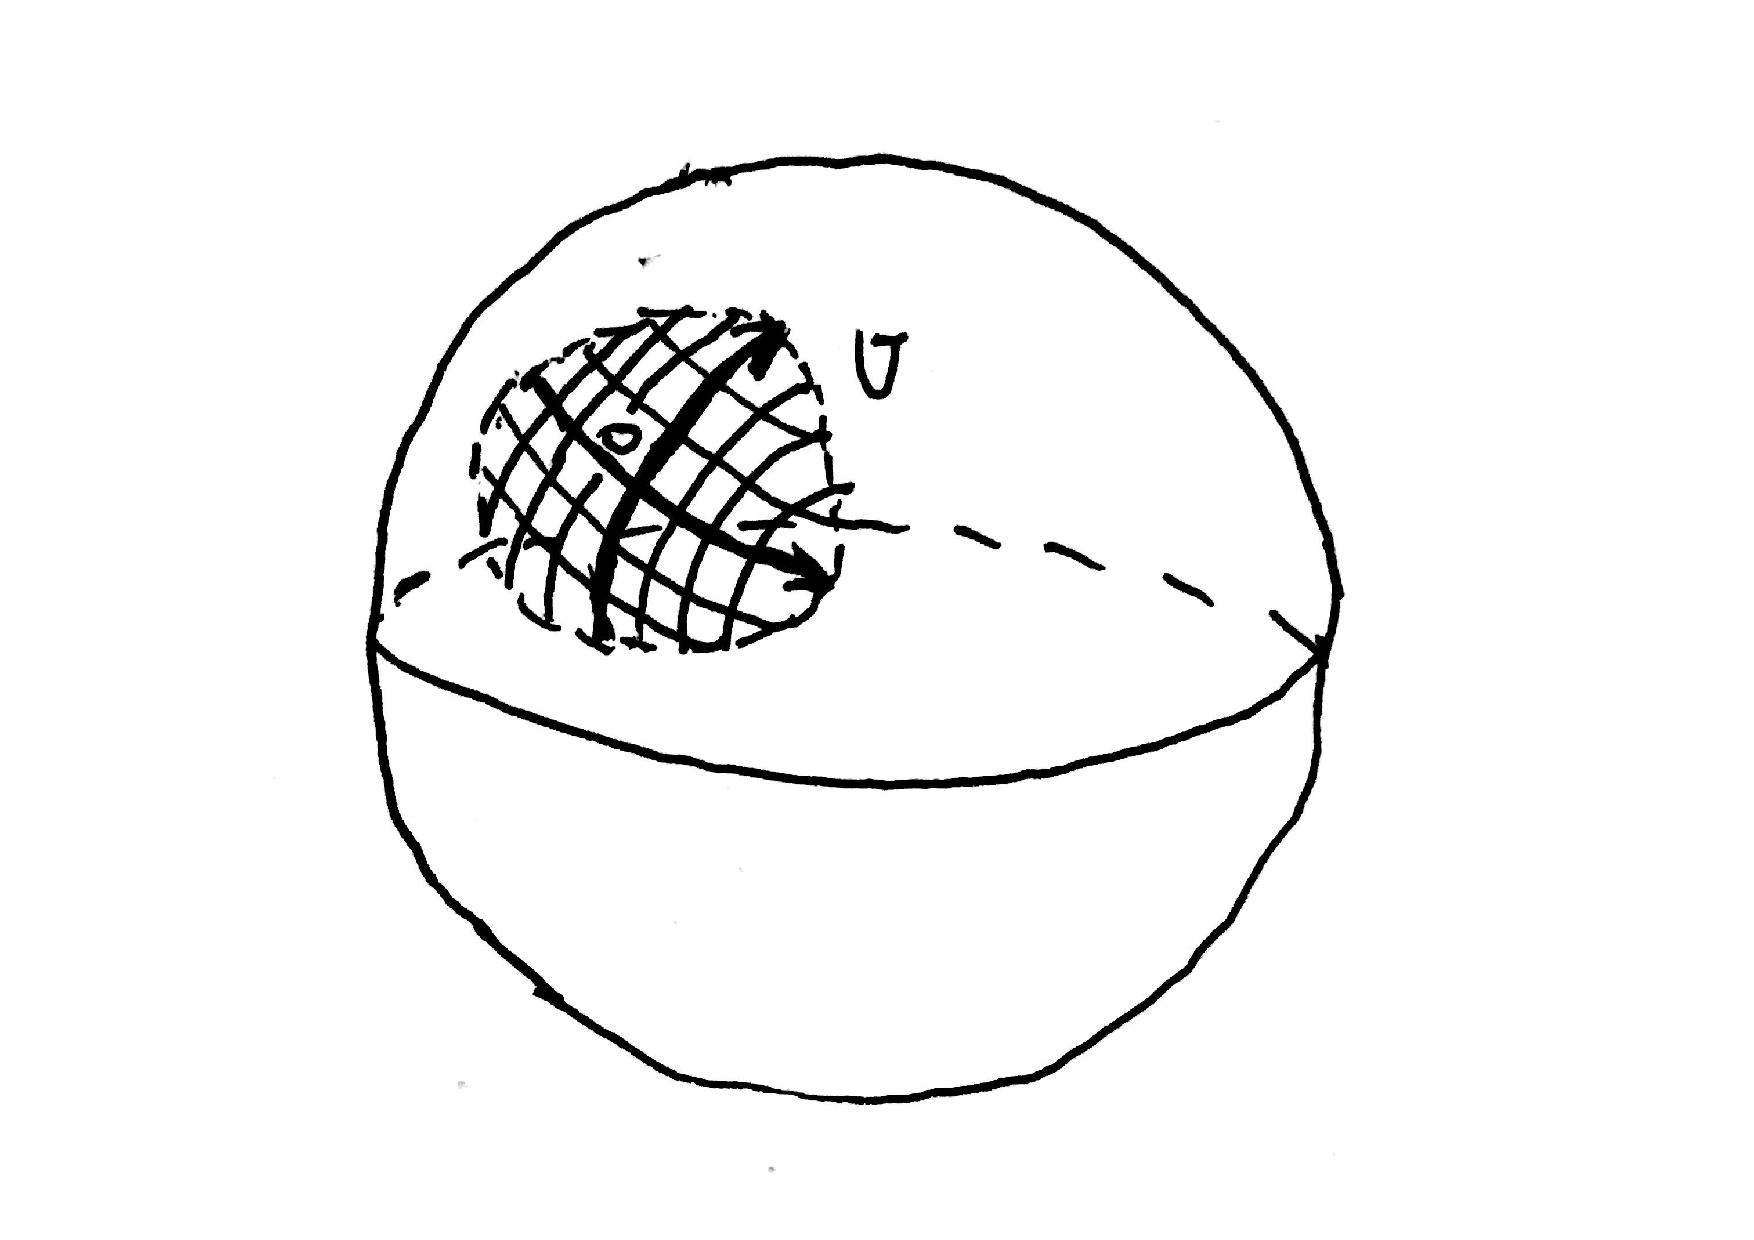
\includegraphics[keepaspectratio, scale=0.3]
         {CoSysInS2.pdf}
    \caption{球面に描かれた局所座標系}
    \label{CoSysInS2}
   \end{figure}
\newpage
%
\section{準備}
\subsection{$m$次元数空間}
\begin{definition}
    $m$を$1$以上の自然数とする. $m$個の実数を
    並べた組
    $$(x_1,x_2, \cdots ,x_m)$$
    の全体からなる集合を$m$次元数空間
    とよび, 記号$\mathbb{R}^m$で
    表す. ただし, $\mathbb{R}^1$は
    $\mathbb{R}$と書くこととする. 

    $\mathbb{R}^m$の元を$\mathbb{R}^m$の点
    とよび, 
    $$\boldsymbol{x}=(x_1,x_2, \cdots ,x_m)$$
    と表す. $x_i$を$\boldsymbol{x}$の第$i$座標
    または第$i$成分という. 

    すべての座標が$0$である点$O
    =(0,\cdots ,0)$を$\mathbb{R}^m$の原点
    という. 
\end{definition}
\begin{definition}
    $\mathbb{R}^m$の$2$点$\boldsymbol{x}
    =(x_1,\cdots ,x_m)$と
    $\boldsymbol{y}
    =(y_1,\cdots ,y_m)$の距離とは
    $$\sqrt{(x_1-y_1)^2+\cdots +(x_m-y_m)^2}$$
    という実数のことである. これを$d(\boldsymbol{x},
    \boldsymbol{y})$という記号で表す. 
\end{definition}
\begin{definition}
    $\boldsymbol{a}$を$\mathbb{R}^m$の$1$点
    , $\epsilon$を正数とする. 点$\boldsymbol{a}$
    の$\mathbb{R}^m$における$\epsilon$-近傍
    $N_\epsilon(\boldsymbol{a};\mathbb{R}^m)$
    とは, $\boldsymbol{a}$からの距離が$\epsilon$
    であるような点$\boldsymbol{x}\in 
    \mathbb{R}^m$の全体のなす集合のことである. 
    すなわち, 
    $$N_\epsilon(\boldsymbol{a};\mathbb{R}^m)=
    \{\boldsymbol{x}\in \mathbb{R}^m
    |d(\boldsymbol{x},\boldsymbol{a})<\epsilon)
    \}$$
    である. $N_\epsilon(\boldsymbol{a};\mathbb{R}^m)$
    を単に$N_\epsilon(\boldsymbol{a})$と書くこともある. 
\end{definition}
\begin{definition}
    $\mathbb{R}^m$の部分集合$U$が$\mathbb{R}^m$
    の開集合であるとは, $U$に含まれる任意の点
    $\boldsymbol{a}$について, $\epsilon>0$を
    十分小さくとると
    $$N_\epsilon(\boldsymbol{a};\mathbb{R}^m)
    \subset U$$
    が成り立つことである. 
    開集合でない部分集合を閉集合という. 
\end{definition}

% \begin{proposition}
%     開集合の基本性質
%     \begin{itemize}
%         \item 
%     \end{itemize}
% \end{proposition}

\subsection{ベクトル空間}\label{def:vector space}
\begin{definition}
    集合$V$が次の条件(I), (II)を満たすとき, 
    $V$を$\mathbb{R}$上のベクトル空間という. 
    \begin{itemize}
        \item[(I)]$V$の$2$元$\boldsymbol{u}$, 
        $\boldsymbol{v}$に対して和とよばれる
        第$3$の元(これを$\boldsymbol{u}+
        \boldsymbol{v}$と表す)が定まり, 
        次の法則が成り立つ.  
        \begin{itemize}
            \item[(1)]
            $(\boldsymbol{u}+
            \boldsymbol{v})+\boldsymbol{w}=
            \boldsymbol{u}+
            (\boldsymbol{v}+\boldsymbol{w})$ 
            (結合法則)
            \item[(2)]
            $\boldsymbol{u}+
            \boldsymbol{v}=
            \boldsymbol{v}+
            \boldsymbol{u}$ 
            (交換法則)
            \item[(3)]
            ゼロベクトルとよばれる元(これを
            $\boldsymbol{o}$と表す)がただひとつ
            存在し, $V$のすべての元$\boldsymbol{v}$
            に対して, 
            $$\boldsymbol{o}+\boldsymbol{v}=
            \boldsymbol{v}$$
            が成り立つ. 
            \item[(4)]
            $V$の任意の元$\boldsymbol{v}$に対し, 
            $\boldsymbol{v}+\boldsymbol{v'}=
            \boldsymbol{o}$となる$V$の元
            $\boldsymbol{v'}$がただひとつ存在する. 
            これを$-\boldsymbol{v}$と表す. 
        \end{itemize} 
        \item[(II)]$V$の任意の元$\boldsymbol{v}$
        と任意の実数$a$に対し, $\boldsymbol{v}$の
        $a$倍とよばれるもうひとつの元(これを
        $a\boldsymbol{v}$と表す)が定まり, 次の
        法則が成り立つ. 
        \begin{itemize}
            \item[(5)]
            $(a+b)\boldsymbol{v}=
            a\boldsymbol{v}+
            b\boldsymbol{v}$,\ 
            \item[(6)]
            $a(\boldsymbol{u}+\boldsymbol{v})=
            a\boldsymbol{u}+a\boldsymbol{v}$,\ 
            \item[(7)]
            $(ab)\boldsymbol{v}=a(b\boldsymbol{v})$,\ 
            \item[(8)]
            $1\boldsymbol{v}=\boldsymbol{v}$. 
        \end{itemize}
    \end{itemize}
    $V$の元をベクトルという. 
\end{definition}
\begin{example}
    $m$次元数空間$\mathbb{R}^m$は($\mathbb{R}$上の)
    ベクトル空間である. 
    $\mathbb{R}^m$の$2$元
    $\boldsymbol{x}=(x_1,\cdots ,x_m)$, 
    $\boldsymbol{y}=(y_1,\cdots ,y_m)$
    に対して和$\boldsymbol{x}+\boldsymbol{y}$
    と$a$倍$a\boldsymbol{x}$を次のように
    定義すればよい. 
    $$\boldsymbol{x}+\boldsymbol{y}=
    (x_1+y_1,\cdots ,x_m+y_m)$$
    $$a\boldsymbol{x}=(ax_1,\cdots ,ax_m)$$
    このように定義したとき, $R^m$が定義\ref{def:vector space}
    の条件(I), (II)を満たすことがわかる. 
    よって, $\mathbb{R}^m$は($\mathbb{R}$上の)
    ベクトル空間である. ただし, ゼロベクトルは
    $\boldsymbol{o}=(0,\cdots ,0)$であり, 
    $-\boldsymbol{x}$は$(-x_1,\cdots ,-x_m)$
    である. ベクトル空間としての$\mathbb{R}^m$
    を($m$次元)数ベクトル空間といい, その元
    $\boldsymbol{x}=(x_1,\cdots ,x_m)$, 
    $\boldsymbol{y}=(y_1,\cdots ,y_m)$
    を($m$次元)数ベクトルという. 
\end{example}
\begin{definition}
    ベクトル空間$V$のいくつかのベクトル
    $\boldsymbol{v_1},\cdots ,
    \boldsymbol{v_k}$について, それぞれを実数倍して加えた和
    $$a_1\boldsymbol{v_1}+\cdots +
    a_k\boldsymbol{v_k}$$
    のことを$\boldsymbol{v_1},\cdots ,
    \boldsymbol{v_k}$の$1$次結合という. 
\end{definition}
\begin{definition}
    $\boldsymbol{v_1},\cdots ,
    \boldsymbol{v_k}$が$1$次独立であるとは, 
    $$a_1\boldsymbol{v_1}+\cdots +
    a_k\boldsymbol{v_k}=\boldsymbol{o}\ 
    \text{ならば}\ a_1=\cdots =a_k=0$$
    が成り立つことである. 
    $\boldsymbol{v_1},\cdots ,
    \boldsymbol{v_k}$が$1$次独立でないとき, 
    それらは$1$次従属であるという. 
\end{definition}
\begin{example}\label{def:fundamental vector of R^m}
    $\mathbb{R}^m$の中の$m$個のベクトル
    $\boldsymbol{e_1},\cdots ,
    \boldsymbol{e_m}$を
    $$e_1=(1,0,\cdots ,0),\ e_2=(0,1,\cdots ,0), 
    \cdots ,e_m=(0,0,\cdots ,1)$$
    と定義すると, これらは$1$次独立である. 
    なぜなら, $\mathbb{R}^m$における和と実数倍の
    定義によって
    $$a_1\boldsymbol{e_1}+\cdots +a_m\boldsymbol{e_m}
    =(a_1,\cdots ,a_m)$$
    となり, $a_1\boldsymbol{e_1}+\cdots +
    a_m\boldsymbol{e_m}=\boldsymbol{o}$
    ならば$a_1=\cdots =a_m=0$でなければならない
    からである. 

    $\boldsymbol{e_i}$を$i$方向の基本ベクトル
    という. 
\end{example}
\begin{definition}\label{def:basis}
    ベクトル空間$V$のベクトルの集合
    $\boldsymbol{f_1},\cdots ,\boldsymbol{f_k}$
    が次の条件(1), (2)を満たすとき, 
    $\boldsymbol{f_1},\cdots ,\boldsymbol{f_k}$
    を$V$の基底とよぶ. 
    \begin{itemize}
        \item[(1)]
        $\boldsymbol{f_1},\cdots ,\boldsymbol{f_k}$
        は$1$次独立である. 
        \item[(2)]
        $V$の任意の元$\boldsymbol{v}$は
        $\boldsymbol{f_1},\cdots ,\boldsymbol{f_k}$
        の$1$次結合として表される. 
    \end{itemize}
\end{definition}
\begin{example}
    $\mathbb{R}^m$の$m$個の基本ベクトル
    $\boldsymbol{e_1},\cdots ,\boldsymbol{e_m}$
    は$\mathbb{R}^m$の基底である. 
    \begin{itemize}
        \item[(1)]
        例\ref{def:fundamental vector of R^m}
        より, 
        $\boldsymbol{e_1},\cdots ,\boldsymbol{e_m}$
        は$1$次独立である. 
        \item[(2)]
        $\mathbb{R}^m$の任意のベクトル$\boldsymbol{x}
        =(x_1,\cdots ,x_m)$
        は$\boldsymbol{e_1},\cdots ,\boldsymbol{e_m}$
        の$1$次結合
        $x_1\boldsymbol{e_1}+\cdots +x_m\boldsymbol{e_m}$
        で表される. 
    \end{itemize}
    よって, $\boldsymbol{e_1},\cdots ,\boldsymbol{e_m}$
    は$\mathbb{R}^m$の基底である.
\end{example}
\begin{definition}
    基底を構成するベクトルの個数$k$を$V$の
    次元とよび, 
    $$k=\text{dim}V$$
    と書く. 
\end{definition}
\begin{definition}
    ベクトル空間$V$の部分集合$W$が次の条件
    (1), (2)を満たすとき, 
    $W
    $を$V$の部分ベクトル空間という. ただし, 
    $W \neq \phi$とする. 
    \begin{itemize}
        \item[(1)]
        $\boldsymbol{u},\ \boldsymbol{v}
        \in W$ならば, 
        $\boldsymbol{u}+\boldsymbol{v}\in W$
        \item[(2)]
        $\boldsymbol{u}\in W$, $a\in \mathbb{R}$
        ならば, $a\boldsymbol{u}\in W$
    \end{itemize}
\end{definition}
ベクトル空間$V$の部分ベクトル空間$W$は
それ自信ベクトル空間である. また, 部分
ベクトル空間$W$の次元は$V$の次元以下である
($\text{dim}W\leq \text{dim}V$). 

\subsection{連続写像と$C^r$級写像}
$U$, $V$をそれぞれ$\mathbb{R}^m$, 
$\mathbb{R}^n$の開集合とする. 
\begin{definition}\label{def:continuous map}
    写像$f:U\to V$が点$\boldsymbol{a}\in U$
    で連続であるとは, $\boldsymbol{a}$
    の像$f(\boldsymbol{a})$の任意の
    $\epsilon$-近傍$N_\epsilon(f(\boldsymbol{a}))$
    に対して, $\delta>0$を十分小さくとれば
    $$f(N_\delta(\boldsymbol{a}))\subset
    N_\epsilon(f(\boldsymbol{a}))$$
    が成り立つことである. 
    $f$が$U$の各点で連続のとき, $f:U\to V$
    を連続写像という. 
\end{definition}
\begin{definition}\label{def:homeomorphism}
    写像$f:U\to V$が次の条件(1), (2)を満たす
    とき, $f$は同相写像であるという. 
    \begin{itemize}
        \item[(1)]
        $f:U\to V$は全単射である. 
        \item[(2)]
        $f:U\to V$も$f^{-1}:V\to U$も, 
        ともに連続写像である. 
    \end{itemize}

    $U$と$V$との間に同相写像$f:U\to V$が
    存在するとき, $U$と$V$は互いに位相同形
    であるといい, 
    $$U \approx V$$
    と書き表す. 
\end{definition}
$f:U\to V$, $g:V\to W$が同相
写像なら逆写像$f^{-1}:V\to U$, 
合成$g\circ f:U\to W$も同相
写像である. 
\begin{definition}\label{def:coordinate display}
    写像$f:U\to V$について, 
    $\boldsymbol{x}\in U$の像$f(\boldsymbol{x})$
    は$V(\subset \mathbb{R}^n)$の点であるから, 
    $f(\boldsymbol{x})=(y_1,\cdots ,y_n)$
    と$\mathbb{R}^n$の座標で書ける. 
    ここで各座標$y_i$の値は$\boldsymbol{x}$によって
    決まるので, $y_i$は$U$上の関数になる. 
    この関数を$f_i$とおくと, 
    $$y_i=f_i(\boldsymbol{x})$$
    であって, $f(\boldsymbol{x})$は
    $$f(\boldsymbol{x})=(f_1(\boldsymbol{x}),
    \cdots ,f_n(\boldsymbol{x}))$$
    と表せる. このような表し方を写像$f:U\to V$
    の座標表示という. 

    $f:U\to V$の座標表示を単に$f=(f_1,\cdots ,f_n)$
    と書くこともある. 
\end{definition}
$f:U\to V$が連続写像であるための必要十分条件は
$f$の座標表示$(f_1,\cdots ,f_n)$に現れる
関数$f_1,\cdots ,f_n$がすべて
連続関数になることである. 
\begin{definition}
    \begin{itemize}
        \item[(1)]
        $r$を自然数($r\geq 1$)とする. $U$上の関数
        $f$が$C^r$級であるとは, $f$の$1$階から
        $r$階までのすべての偏導関数
        $\frac{\partial f}{\partial x_i},\cdots ,
        \frac{\partial^rf}{\partial x_i^r}\ 
        (i=1,\cdots m)$が存在して$f$自信も含めて
        それらがみな$U$上で連続であることをいう. 
        \item[(2)]
        $f$が任意の自然数$r$について$C^r$級
        であるとき, $f$を$C^\infty$級関数でという. 
    \end{itemize}
    なお, 連続関数のことを$C^0$級関数ということがある. 
\end{definition}
\begin{definition}\label{def:C^r map}
    写像$h:U\to V$が$C^r$級写像であるとは, 
    $h$の座標表示$h=(h_1,\cdots ,h_n)$に現れる
    関数$h_1,\cdots ,h_n$がすべて$U$上の$C^r$級
    関数になることである. 
\end{definition}
\begin{proposition}
    $C^r$級関数の$1$次結合や積は$C^r$級
    関数である(ただし, $0\leq r\leq \infty$). 
\end{proposition}
\begin{proposition}
    写像$h:U\to V$の座標表示
    に現れる関数$h_1,\cdots ,h_n$と
    $V$上の関数$f$が$C^1$級関数である
    とすると, 合成関数$f\circ h$も
    $C^1$級であり, かつ次の公式
    (合成関数の微分法)が成り立つ. 
    $$\frac{\partial (f\circ h)}{\partial x_i}=
    \left(\frac{\partial f}{\partial y_1}
    \circ h\right)\cdot \frac{\partial h_1}
    {\partial x_i}+\cdots +
    \left(\frac{\partial f}{\partial y_n}
    \circ h\right)\cdot \frac{\partial h_n}
    {\partial x_i}$$
    ただし, ふつうは簡単に
    $$\frac{\partial (f\circ h)}{\partial x_i}=
    \left(\frac{\partial f}{\partial y_1}
    \right)\cdot \frac{\partial h_1}
    {\partial x_i}+\cdots +
    \left(\frac{\partial f}{\partial y_n}
    \right)\cdot \frac{\partial h_n}
    {\partial x_i}$$
    と書くこととする. 
\end{proposition}
\begin{proposition}
    $h:U\to V$が$C^r$級写像, $f:V\to \mathbb{R}$
    が$C^r$級関数なら, 合成関数$f\circ h:U\to 
    \mathbb{R}$も$C^r$級関数である(ただし, 
    $0\leq r\leq \infty$). 
\end{proposition}
\begin{proposition}
    $U$, $V$, $W$がそれぞれ$\mathbb{R}^m$, 
    $\mathbb{R}^n$, $\mathbb{R}^l$
    の開集合のとき, $2$つの$C^r$級
    写像$f:U\to V$, $g:V\to W$の合成写像
    $g\circ f:U\to W$は$C^r$級である. 
\end{proposition}
\begin{definition}\label{def:C^r diffeomorphism}
    写像$f:U\to V$が次の条件(1), (2)を満たすとき, 
    $f$を$C^r$級微分同相写像という. 
    \begin{itemize}
        \item[(1)]
        $f:U\to V$は全単射である. 
        \item[(2)]
        $f:U\to V$も$f^{-1}:V\to U$もともに
        $C^r$級写像である. 
    \end{itemize}

    $U$と$V$との間に$C^r$級微分同相写像
$f:U\to V$が存在するとき, $U$と$V$は互いに
$C^r$級微分同相であるという.
\end{definition}
$f:U\to V$, $g:V\to W$が$C^r$級微分同相
写像なら逆写像$f^{-1}:V\to U$, 
合成$g\circ f:U\to W$も$C^r$級微分同相
写像である. 
 
\subsection{位相空間}
\begin{definition}\label{def:topological sapace}
    集合$X$び部分集合族$\mathcal{O}$が次の条件
    (1), (2), (3)を満たすとき, $\mathcal{O}$
    を$X$の位相とよび, $X$と$\mathcal{O}$の対
    $(X,\mathcal{O})$を位相空間という. 
    \begin{itemize}
        \item[(1)]$X\in \mathcal{O}$かつ
        $\phi \in \mathcal{O}$
        \item[(2)]
        $U_1,U_2, \cdots ,U_k\in \mathcal{O}$
        ならば$U_1\cap U_2\cap \cdots \cap U_k
        \in \mathcal{O}$
        \item[(3)]
        任意の集合族$\{U_\lambda\}_\Lambda$について
        $U_\lambda\in \mathcal{O}\ 
        (\forall \lambda \in \Lambda)$ならば
        $$\bigcup_{\lambda\in \Lambda}{U_\lambda}
        \in \mathcal{O}$$
    \end{itemize}
    位相$\mathcal{O}$を位相空間$X$の
    開集合系とよぶことがある. $X$の部分集合
    $U$が$\mathcal{O}$に属するとき, $U$を
    $X$の開集合という. 
    位相空間$X$の個々の元を$X$の点という. 
\end{definition}
\begin{example}
    $m$次元数空間$\mathbb{R}^m$の開集合全体の
    なす集合族を$\mathcal{O}^{(m)}$とする. 
    このとき, $\mathcal{O}^{(m)}$は
    上の定義\ref{def:topological sapace}
    の条件(1), (2), (3)を満たす
    (ただし, $X=\mathbb{R}^m$). したがって, 
    $\mathcal{O}^{(m)}$は$\mathbb{R}^m$
    の位相であり, $(\mathbb{R}^m, \mathcal{O}^{(m)})$
    は位相空間である.

    $\mathcal{O}^{(m)}$を$\mathbb{R}^m$の自然な
    位相という. 通常, $\mathbb{R}^m$を位相空間と
    考えるときは, この位相$\mathcal{O}^{(m)}$
    が指定されているものとする. 
\end{example}
\begin{definition}
    $(X, \mathcal{O})$を位相空間, $A$を
    $X$の任意の部分空間とすると, $A$の部分集合族
    $$\mathcal{O}_A=\{U\cap A|U\in \mathcal{O}\}$$
    を$A$の位相として, $A$をそれ自身ひとつの位相空間
    と考えることができる. 

    この$\mathcal{O}_A$を$X$の位相$\mathcal{O}$
    から導かれた$A$の相対位相とよび, 位相空間
    $(A,\mathcal{O}_A)$を$(X,\mathcal{O})$の
    部分空間とよぶ. 
\end{definition}
\begin{figure}[H]
    \centering
    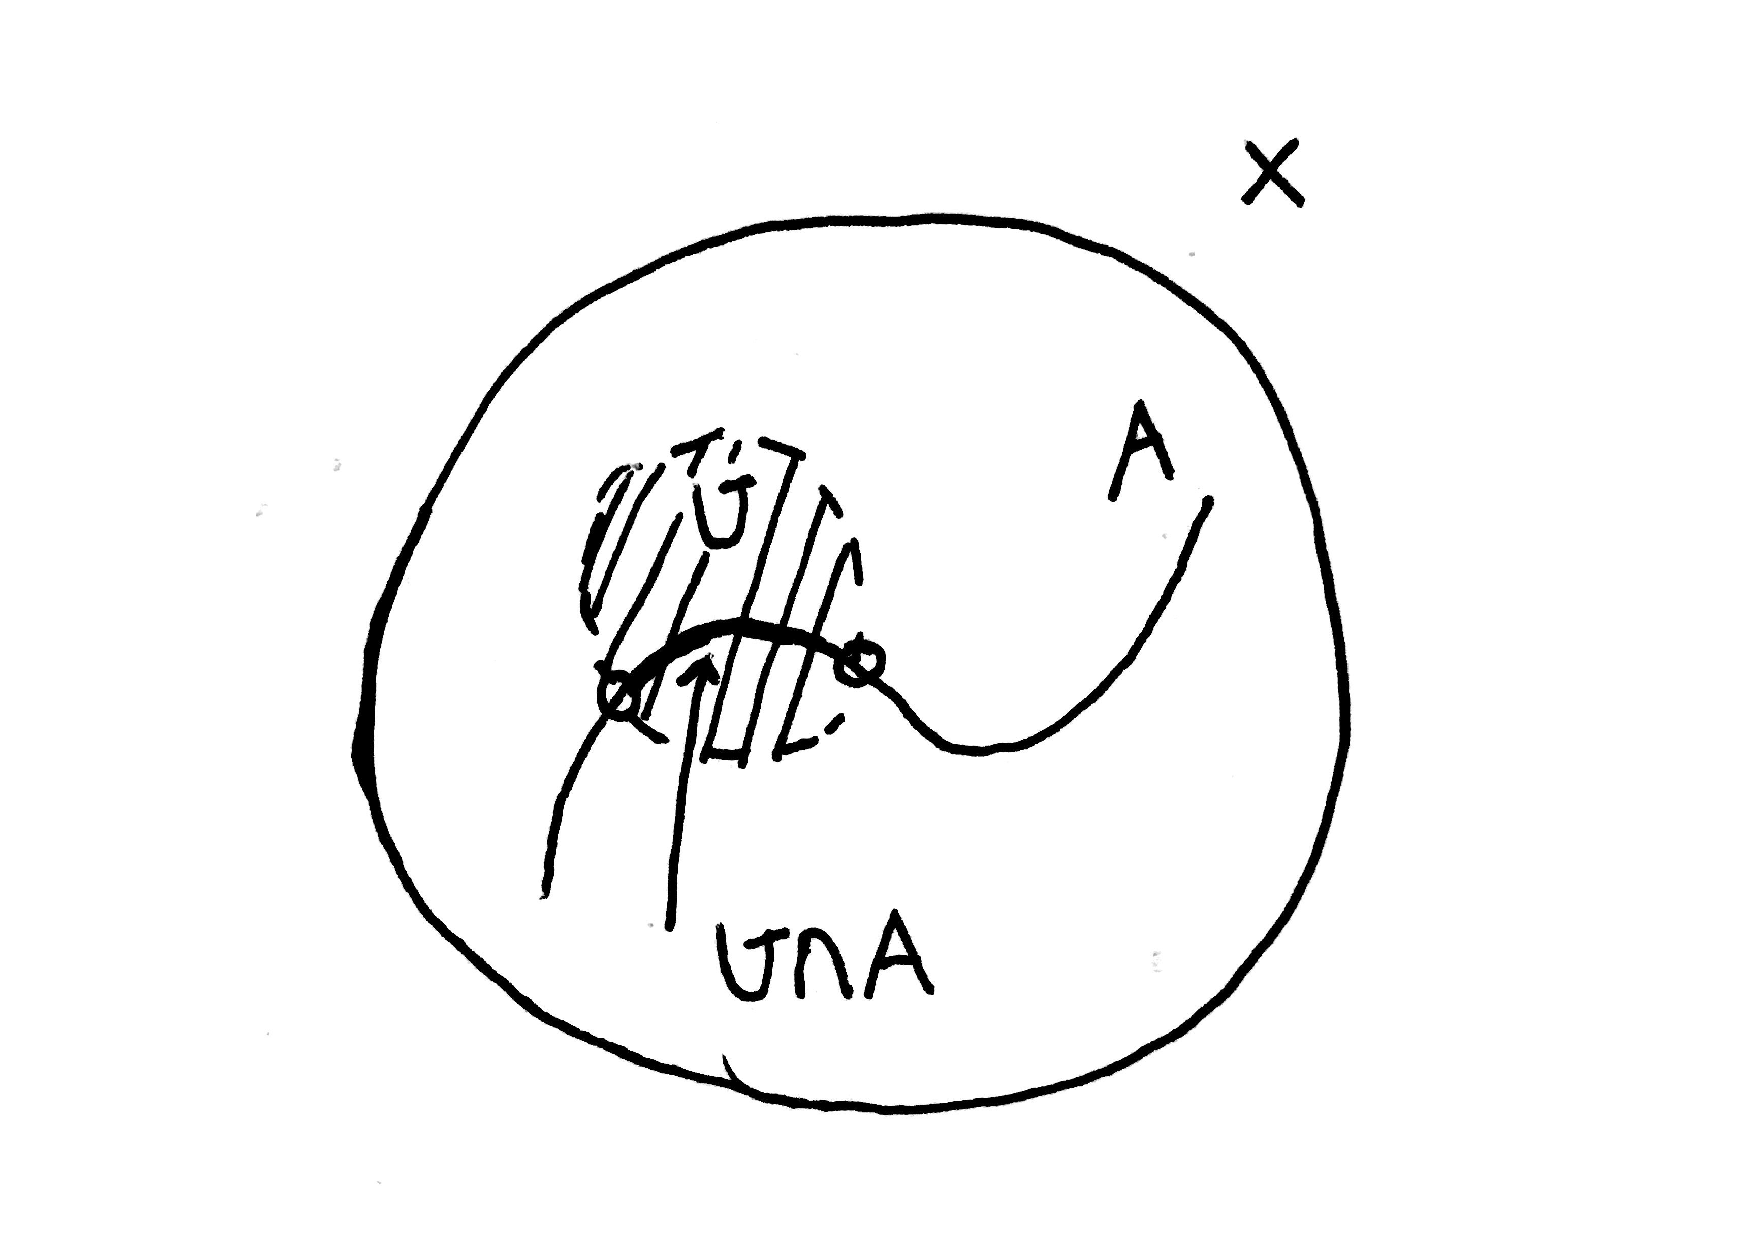
\includegraphics[keepaspectratio, scale=0.3]{relativeTopology.pdf}
    \caption{$A$の相対位相}
    \label{relativeTopology}
   \end{figure}
   
\begin{definition}\label{def:topological continuous map}
$2$つの位相空間$(X, \mathcal{O})$, $(Y,\mathcal{O}')$
の間の写像$f:X\to Y$が連続写像であるとは, $Y$の任意の
開集合$U$について, $f^{-1}(U)\in \mathcal{O}$
となることである. 

一般に逆像$f^{-1}(U)$とは
$$f^{-1}(U)=\{p\in X|f(p)\in U\}$$
で定義される$X$の部分集合のことである. 
\end{definition}
位相空間$X$, $Y$をそれぞれ$\mathbb{R}^m$, 
$\mathbb{R}^n$の開集合$V$, $W$とすると
上の定義\ref{def:topological continuous map}の
連続写像の概念と, 定義\ref{def:continuous map}
の連続写像の概念は一致する. 
\begin{definition}\label{def:topological homeomorphism}
    位相空間$(X,\mathcal{O})$, $(Y,\mathcal{O}')$
    の間の写像$f:X\to Y$が次の条件(1), (2)を満たす
    とき, $f$を同相写像という. 
    \begin{itemize}
        \item[(1)]$f:X\to Y$は全単射である. 
        \item[(2)]$f:X\to Y$も$f^{-1}:Y\to X$
        もともに連続写像である. 

        $X$と$Y$との間に同相写像$f:X\to Y$が
    存在するとき, $X$と$Y$は互いに位相同形
    であるといい, 
    $$X \approx Y$$
    と書き表す. 
    \end{itemize}
\end{definition}
明らかに, この定義\ref{def:topological homeomorphism}
は定義\ref{def:homeomorphism}の拡張である. 

また, $f:X\to Y$, $g:Y\to Z$が同相写像なら
逆写像$f^{-1}:Y\to X$, 
合成$g\circ f:X\to Z$も同相写像である. 

\begin{definition}\label{def:hausdorff space}
    位相空間$(X,\mathcal{O})$の任意の異なる$2$
    点$p$, $q$に対して, $p$を含む開集合$U$と
    $q$を含む開集合$V$が存在して
    $$U\cap V=\phi$$
    を満たすとき, 
    $(X,\mathcal{O})$をハウスドルフ空間という. 
\end{definition}
\newpage
%
\section{$C^r$級多様体と$C^r$級写像}
\subsection{$C^r$級多様体}
\begin{definition}
    位相空間$X$の開集合$U$から$m$次元数空間$\mathbb{R}^m$
    のある開集合$U'$への同相写像
    $$\varphi:U\rightarrow U'$$
    があるとき, $(U, \varphi)$を$m$次元座標近傍といい, 
    $\varphi$を$U$上の局所座標系という. 
\end{definition}
\begin{figure}[H]
    \centering
    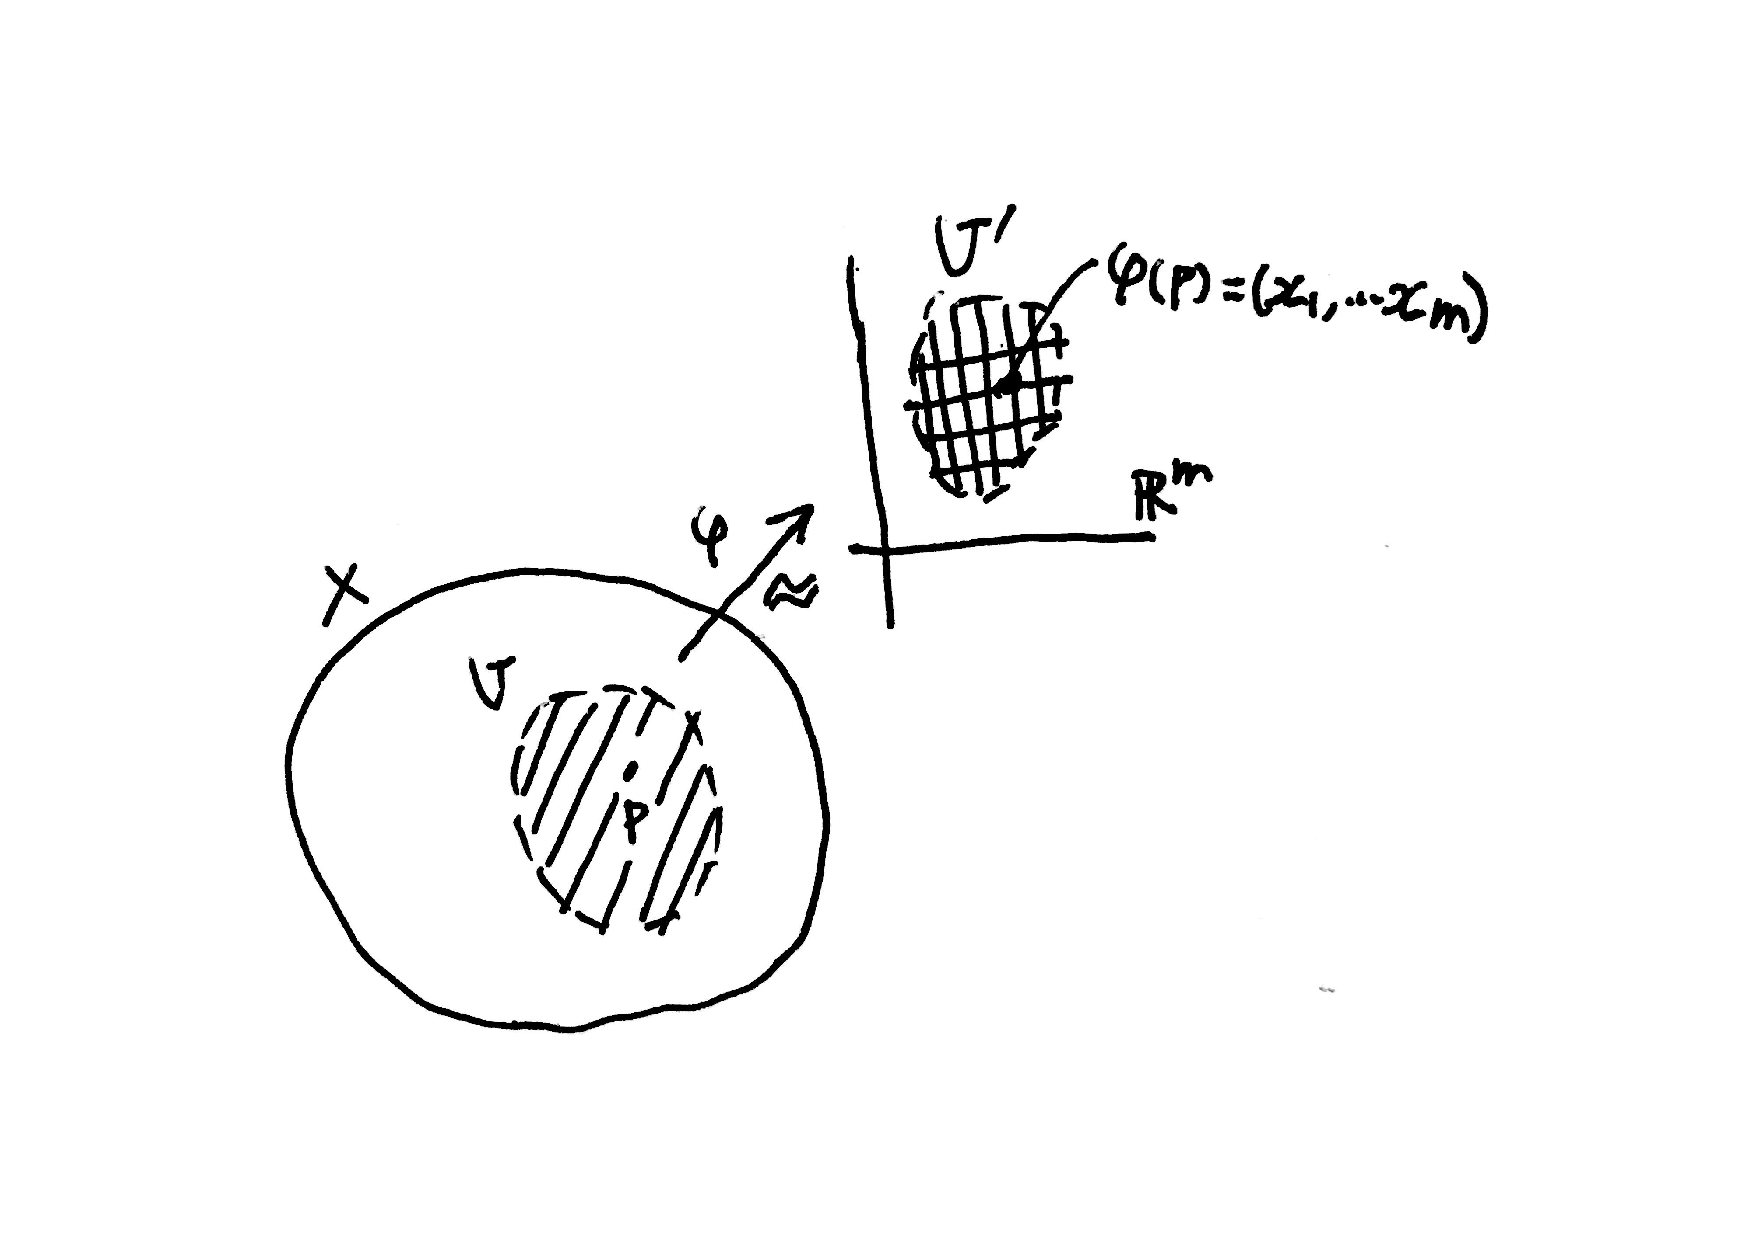
\includegraphics[keepaspectratio, scale=0.4]
    {coNeighborhoodBig.pdf}
    \caption{$U$上の局所座標系}
    \label{coNeighborhood}
   \end{figure}
$(U,\varphi)$には局所座標系$(x_1, \cdots ,x_m)$
    が描かれていると考え, $(U;x_1, \cdots ,x_m)$
    とも表すこととする. 
    \begin{figure}[H]
        \centering
        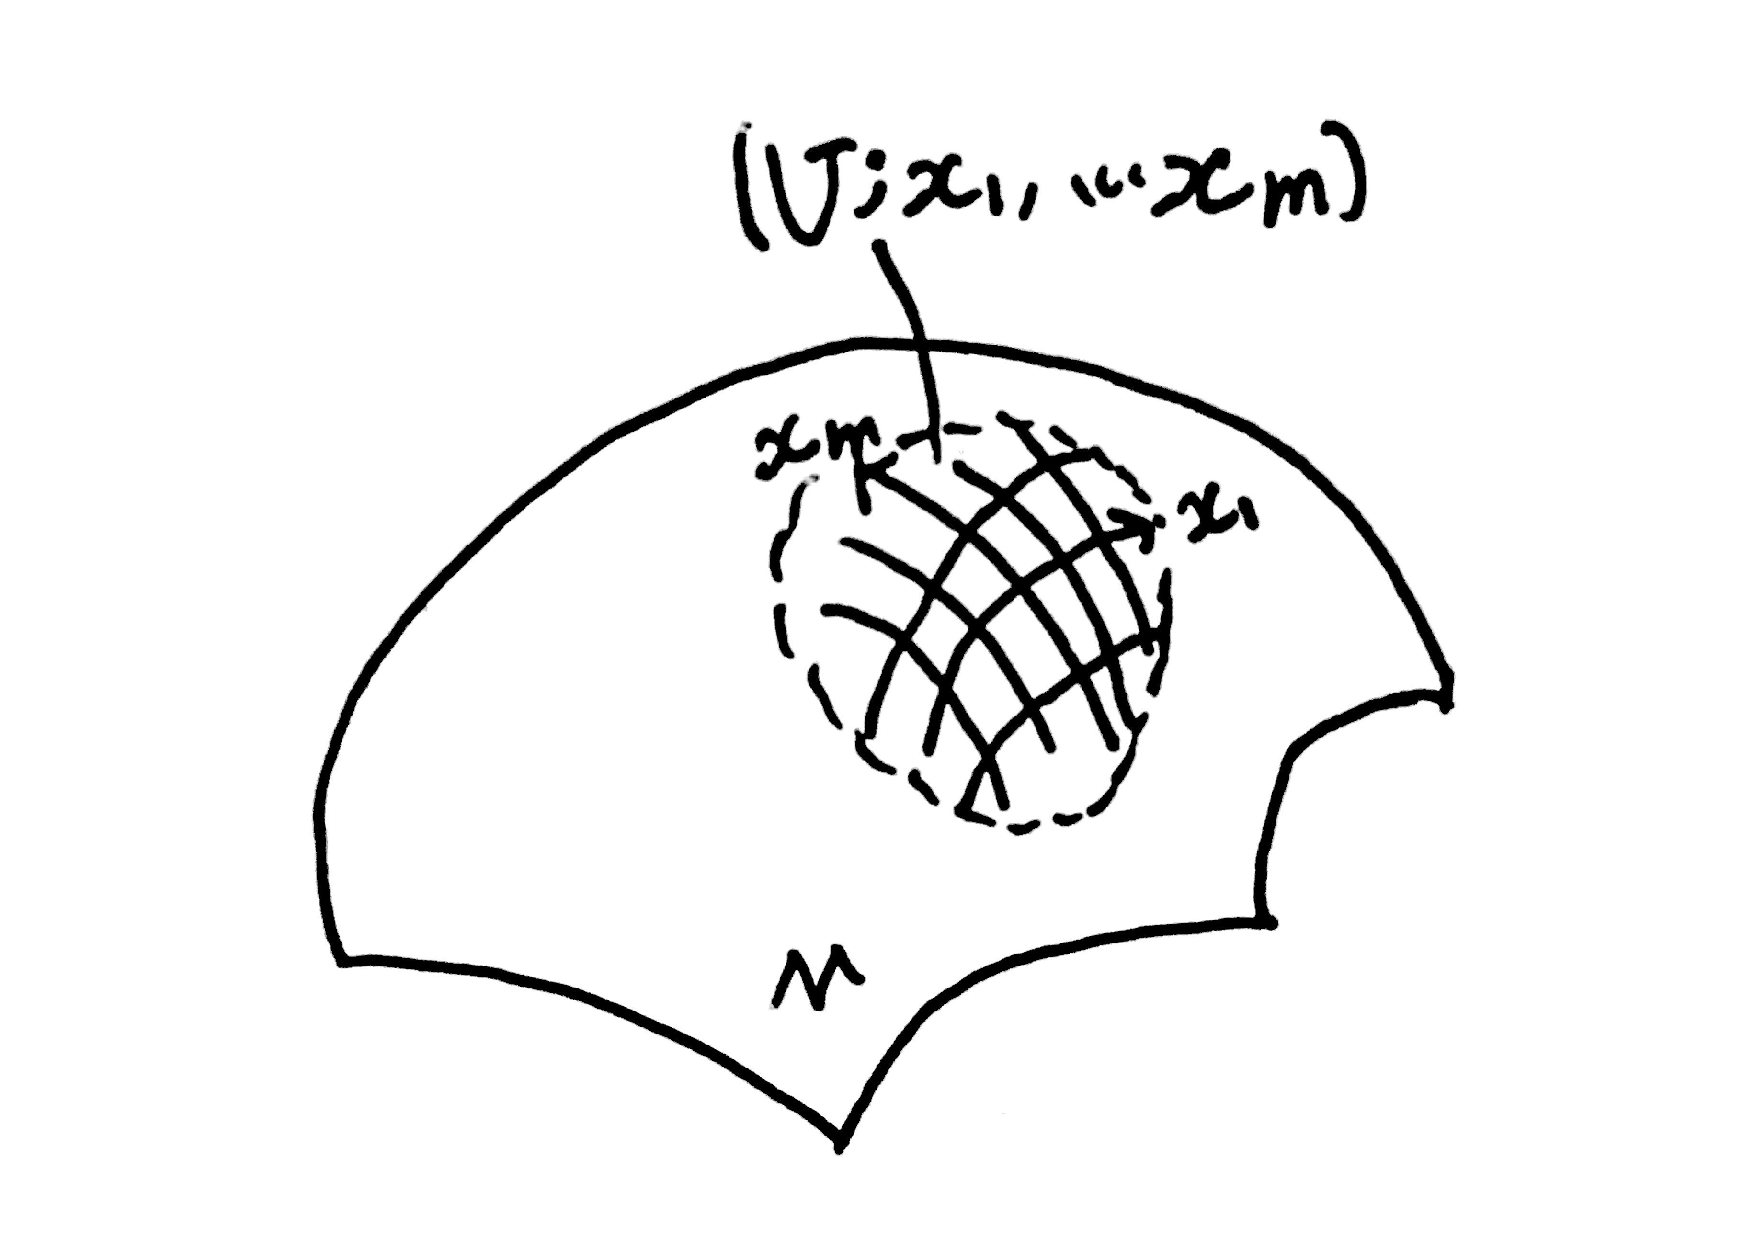
\includegraphics[keepaspectratio, scale=0.2]{DrawnLocalCoSysBig.pdf}
        \caption{$U$上に描かれた局所座標系}
        \label{DrawnLocalCoSysd}
       \end{figure}
\begin{definition}
    $(U, \varphi)$を位相空間$X$内の局所座標近傍とする.
    $U$内の任意の点$p$に対して$\varphi(p) \in \mathbb{R}^m$
    であるから, 
    $$\varphi(p)=(x_1, \cdots ,x_m)$$
    と書ける.$(x_1, \cdots ,x_m)$を$(U, \varphi)$に関する$p$
    の局所座標という.
\end{definition}
\begin{definition}
    位相空間$M$が次の条件(1),(2)を満たすとき, 
    $M$を$m$次元位相多様体という. 
    \begin{itemize}
        \item[(1)]$M$はハウスドルフ空間である.
        \item[(2)]$M$内の任意の点$p$に対して, 
        $p$を含む$m$次元座標近傍$(U,\varphi)$が存在する.
    \end{itemize}
\end{definition}
\begin{definition}
    $m$次元位相多様体$M$の$2$つの座標近傍$(U, \varphi)$, 
    $(V, \psi)$が交わっているとき, 同相写像
    $$\psi \circ \varphi^{-1}:\varphi(U\cap V)\rightarrow \psi(U\cap V)$$
    を$(U, \varphi)$から$(V, \psi)$への座標変換という. 
\end{definition}
\begin{figure}[H]
    \centering
    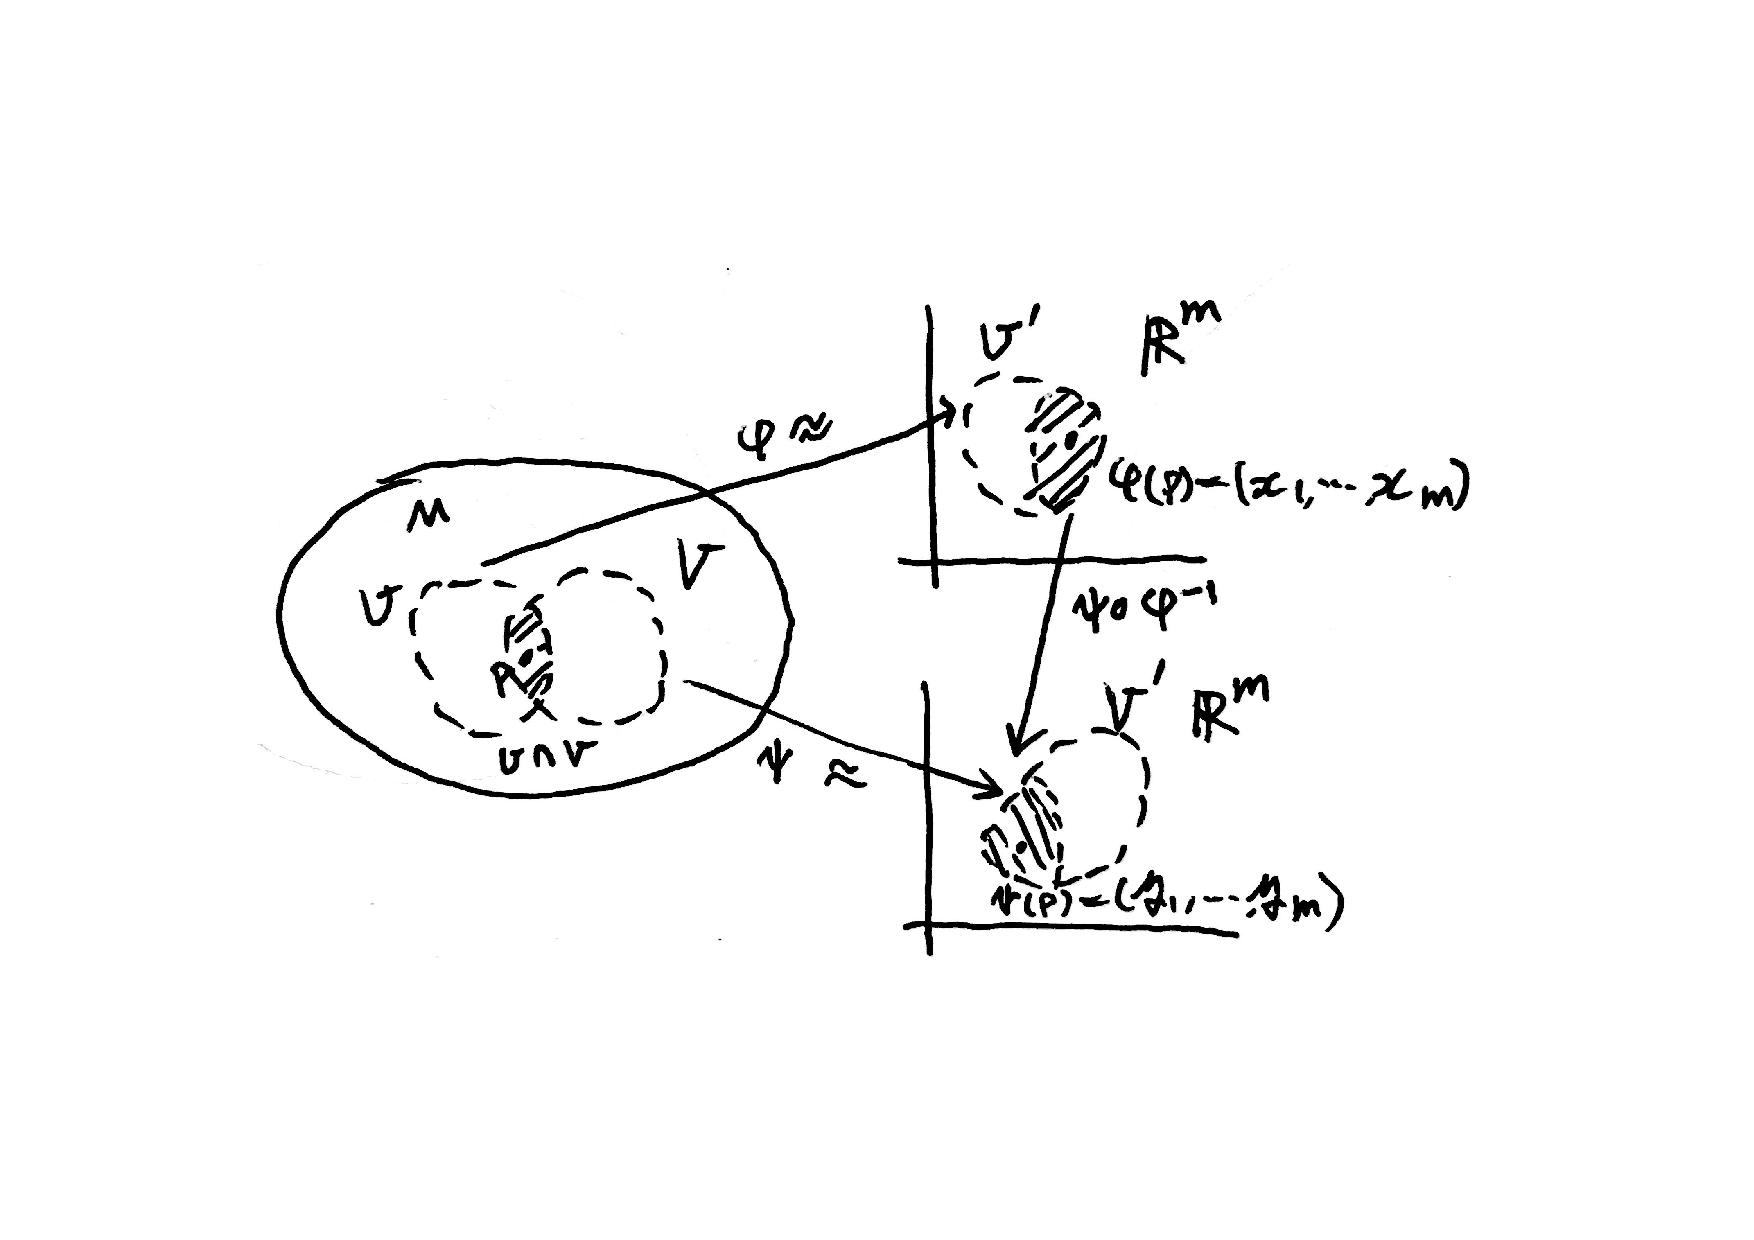
\includegraphics[keepaspectratio, scale=0.5]{coordinateConversionBig.pdf}
    \caption{座標変換$\psi \circ \varphi^{-1}$}
    \label{coordinateConversion}
   \end{figure}
   
\begin{definition}\label{def:C^r manifold}
    $r\geq 1$を自然数または$\infty$とする. 
    位相空間$M$が次の条件(1), (2), (3)を満たすとき, 
    $M$を$m$次元$C^r$級多様体という.
    \begin{itemize}
        \item[(1)]$M$はハウスドルフ空間である.
        \item[(2)]$M$は$m$次元座標近傍により被覆される. 
        すなわち, $M$の$m$次元座標近傍からなる族
        $\{(U_\alpha, \varphi_\alpha)\}_{\alpha \in A}$
        があって, 
        $$M = \bigcup_{\alpha \in A}U_\alpha$$
        が成り立つ. 
        \item[(3)]$U_\alpha \cap U_\beta \neq \phi$
        であるような任意の$\alpha$, $\beta$に対して, 座標変換
        $$\varphi_\beta \circ \varphi_\alpha^{-1}:
        \varphi_\alpha(U_\alpha\cap U_\beta)\rightarrow 
        \varphi_\beta(U_\alpha\cap U_\beta)$$
        は$C^r$級写像である. 
    \end{itemize}
\end{definition}
\begin{theorem}
    $m$次元球面$S^m \in \mathbb{R}^{m+1}$を
    $$S^m=\{(x_1,\cdots x_{m+1})|x_1^2+\cdots +x_{m+1}^2=1\}$$
    と定義すると, $S^m$は$m$次元$C^{\infty}$級多様体である. 
\end{theorem}
\begin{proof}
    定義\ref{def:C^r manifold}の条件(1), (2), (3)を確かめる. 
    \begin{itemize}
        \item[(1)]$\mathbb{R}^{m+1}$はハウスドルフ空間
        であるから, その部分空間として, $S^m$は
        ハウスドルフ空間である. 
        \item[(2)]$S^m$の$2(m+1)$個の開集合
        $U_i^+$, $U_i^-$ $(i=1,\cdots ,m+1)$を
        次のように定義する. 
        $$U_i^+ = \{(x_1, \cdots x_i, \cdots ,x_{m+1})\in S^m|x_i>0\}$$
        $$U_i^- = \{(x_1, \cdots x_i, \cdots ,x_{m+1})\in S^m|x_i<0\}$$
        $S^m$はこれら$U_i^+$, $U_i^-$ $(i=1,\cdots ,m+1)$
        で被覆される. 写像$\varphi_i^+:U_i^+ \rightarrow \mathbb{R}^m$, 
        $\varphi_i^-:U_i^- \rightarrow \mathbb{R}^m$を
        それぞれ次のように定義する. 
        $$\varphi_i^+(x_1,\cdots ,x_i,\cdots, x_{m+1})=(x_1,\cdots ,\hat{x_i},\cdots ,x_{m+1})$$
        $$\varphi_i^-(x_1,\cdots ,x_i,\cdots, x_{m+1})=(x_1,\cdots ,\hat{x_i},\cdots ,x_{m+1})$$
        ここで, $\hat{x_i}$は$x_i$を取り去るという意味である. このとき, 
        $$(\varphi_i^+)^{-1}(x_1,\cdots ,\hat{x_i},\cdots ,x_{m+1})=(x_1,\cdots ,\sqrt{1-||(x_1,\cdots ,\hat{x_i},\cdots ,x_{m+1})||^2},\cdots ,x_{m+1})$$
        $$(\varphi_i^-)^{-1}(x_1,\cdots ,\hat{x_i},\cdots ,x_{m+1})=(x_1,\cdots ,-\sqrt{1-||(x_1,\cdots ,\hat{x_i},\cdots ,x_{m+1})||^2},\cdots ,x_{m+1})$$
        であり, $\varphi_i^+$, $\varphi_i^-$はそれぞれ, $U_i^+$, 
        $U_i^-$から$\mathring{D}^m$への同相写像である.
        ただし, $\mathring{D}^m$は$\mathbb{R}^m$の原点を
        中心とするm次元単位開円板である. 
        よって, $S^m$は$2(m+1)$個の座標近傍$(U_1^+,\varphi_1^+),
        (U_1^-,\varphi_1^-),\cdots ,(U_{m+1}^+,\varphi_{m+1}^+),(U_{m+1}^-,\varphi_{m+1}^-)$
        で被覆される. 
        \item[(3)]$2(m+1)$個の座標近傍の間の座標変換がすべて
        $C^{\infty}$級であることを示す. \\
        $1\leq a, b\leq 2(m+1)$を満たす互いに異なる自然数$a$, $b$
        に対して, 
        \begin{itemize}
            \item[(i)]$(U_a^+,\varphi_a^+)$と$(U_b^+,\varphi_b^+)$
            \item[(ii)]$(U_a^-,\varphi_a^-)$と$(U_b^-,\varphi_b^-)$
            \item[(iii)] $(U_a^+,\varphi_a^+)$と$(U_b^-,\varphi_b^-)$ 
        \end{itemize}
        の間の座標変換を調べればよい. \\
        (i)の場合, 
        \begin{eqnarray*}
            &&U_a^+\cap U_b^+ =\{(x_1,\cdots ,x_a,\cdots ,x_b,\cdots ,x_{m+1})\in S^m|x_a>0,\ x_b>0\}\\
            &&\varphi_a^+(U_a^+\cap U_b^+) =\{(x_1,\cdots ,\hat{x_a},\cdots ,x_b,\cdots ,x_{m+1})\in \mathring{D}^m|x_b>0\}\\
            &&\varphi_b^+(U_a^+\cap U_b^+) =\{(x_1,\cdots ,x_a,\cdots ,\hat{x_b},\cdots ,x_{m+1})\in \mathring{D}^m|x_a>0\}\\
            &&(\varphi_a^+)^{-1}x_1,\cdots ,\hat{x_a},\cdots ,x_b,\cdots x_{m+1})\\
            &&=(x_1,\cdots ,\sqrt{1-||(x_1,\cdots ,\hat{x_a},\cdots ,x_b,\cdots x_{m+1})||^2},\cdots ,x_b,\cdots x_{m+1})
        \end{eqnarray*}
        この式から
        \begin{eqnarray*}
        &&\varphi_b^+\circ(\varphi_a^+)^{-1}(x_1,\cdots ,\hat{x_a},\cdots ,x_b,\cdots ,x_{m+1})\\
        &&=(x_1,\cdots ,\sqrt{1-||(x_1,\cdots ,\hat{x_a},\cdots ,x_b,\cdots ,x_{m+1})||^2},\cdots ,\hat{x_b},\cdots ,x_{m+1})
        \end{eqnarray*}
        これは$||(x_1,\cdots ,\hat{x_a},\cdots ,x_b,\cdots ,x_{m+1})||^2<1$の
        範囲で$C^{\infty}$級なので, \\$\varphi_b^+\circ(\varphi_a^+)^{-1}$
        は定義域$\varphi_a^+(U_a^+\cap U_b^+)\subset \mathring{D}^m$
        で$C^{\infty}$級である. \\
        同様にして(ii), (iii)の場合についても座標変換が$C^{\infty}$級である
        こと分かる. \\
    \end{itemize}
    以上より, $S^m$は$m$次元$C^{\infty}$級多様体であることが分かった. 
\end{proof}
以下は$S^1$の場合の開集合と局所座標系である. 
\begin{figure}[H]
    \begin{tabular}{cc}
      %---- 最初の図 ---------------------------
      \begin{minipage}[t]{0.45\hsize}
        \centering
        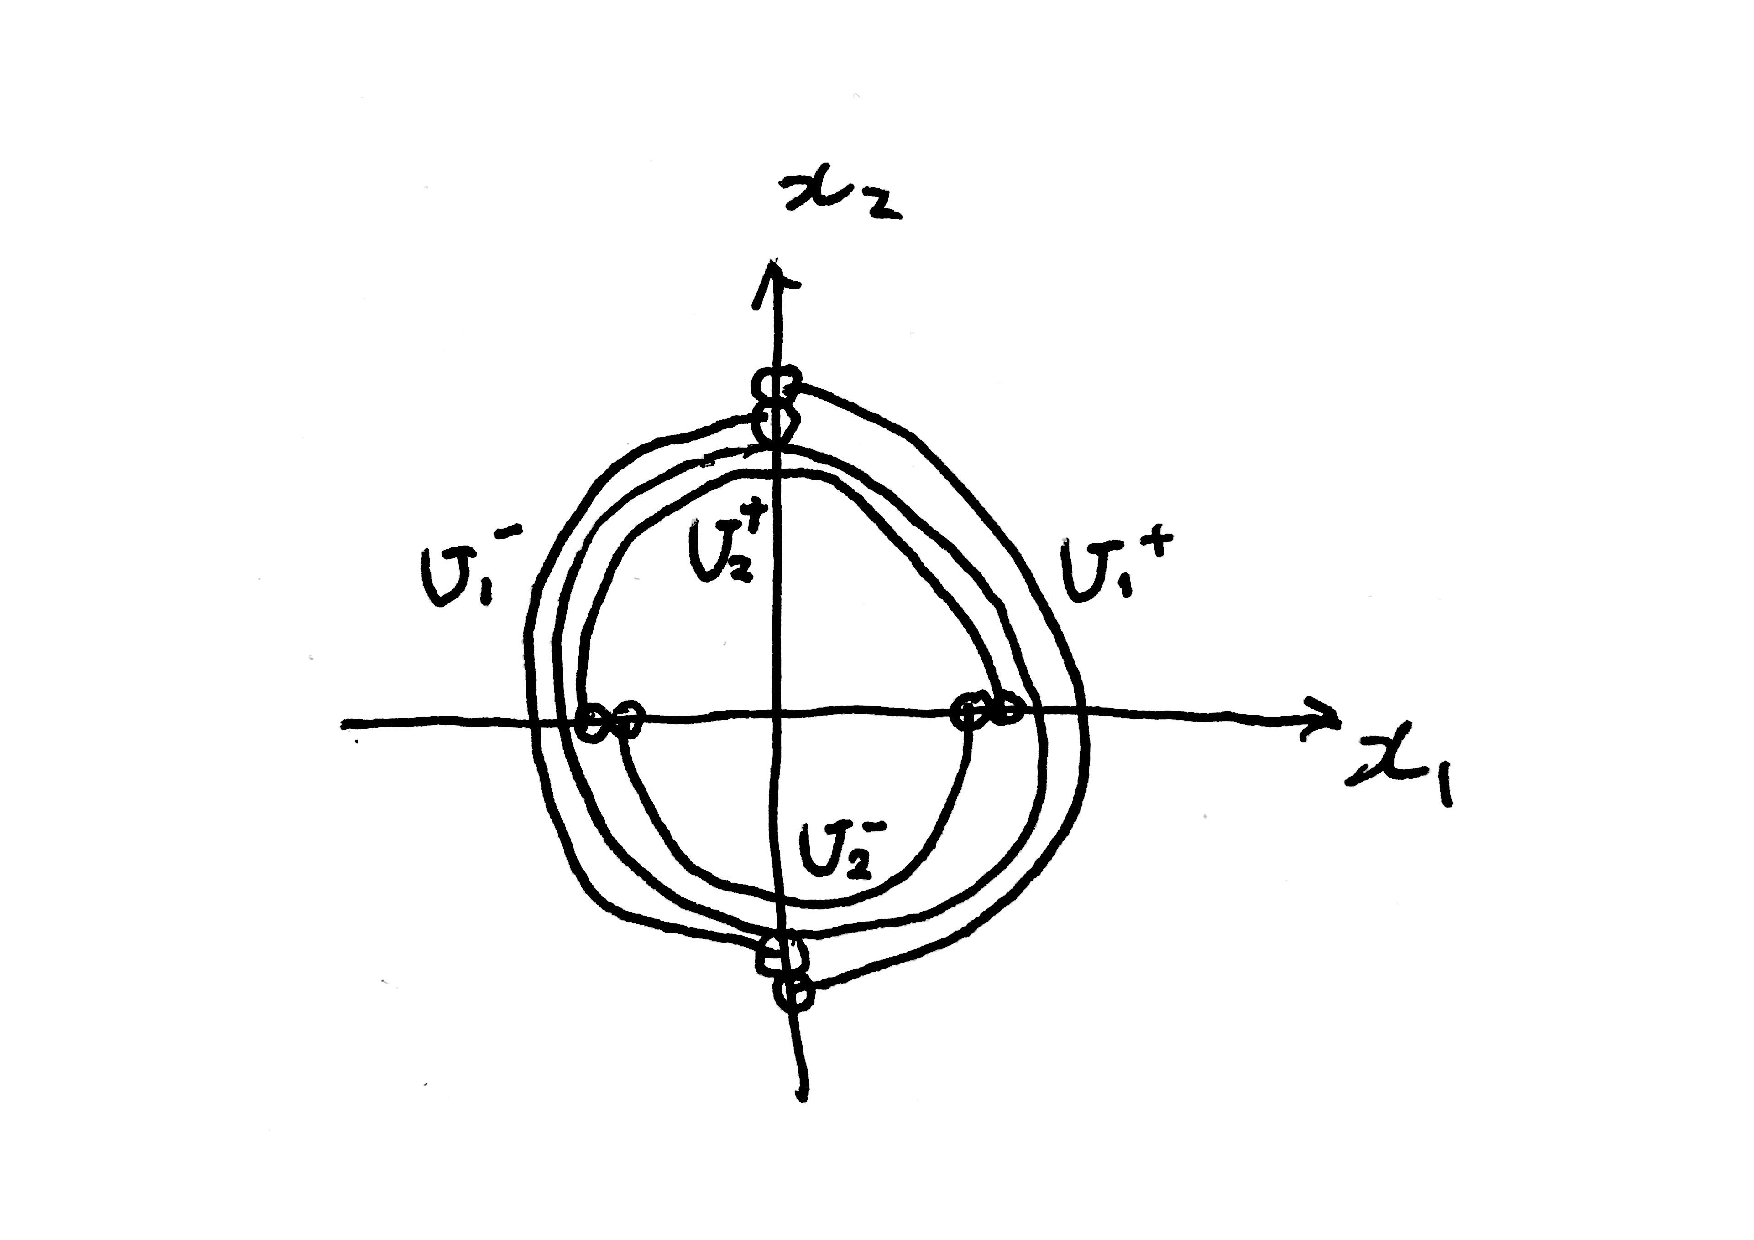
\includegraphics[keepaspectratio, scale=0.2]{localCoSysOfS1_1.pdf}
        \caption{$S^1$の開集合}
        \label{}
      \end{minipage} &
      %---- 2番目の図 --------------------------
      \begin{minipage}[t]{0.45\hsize}
        \centering
        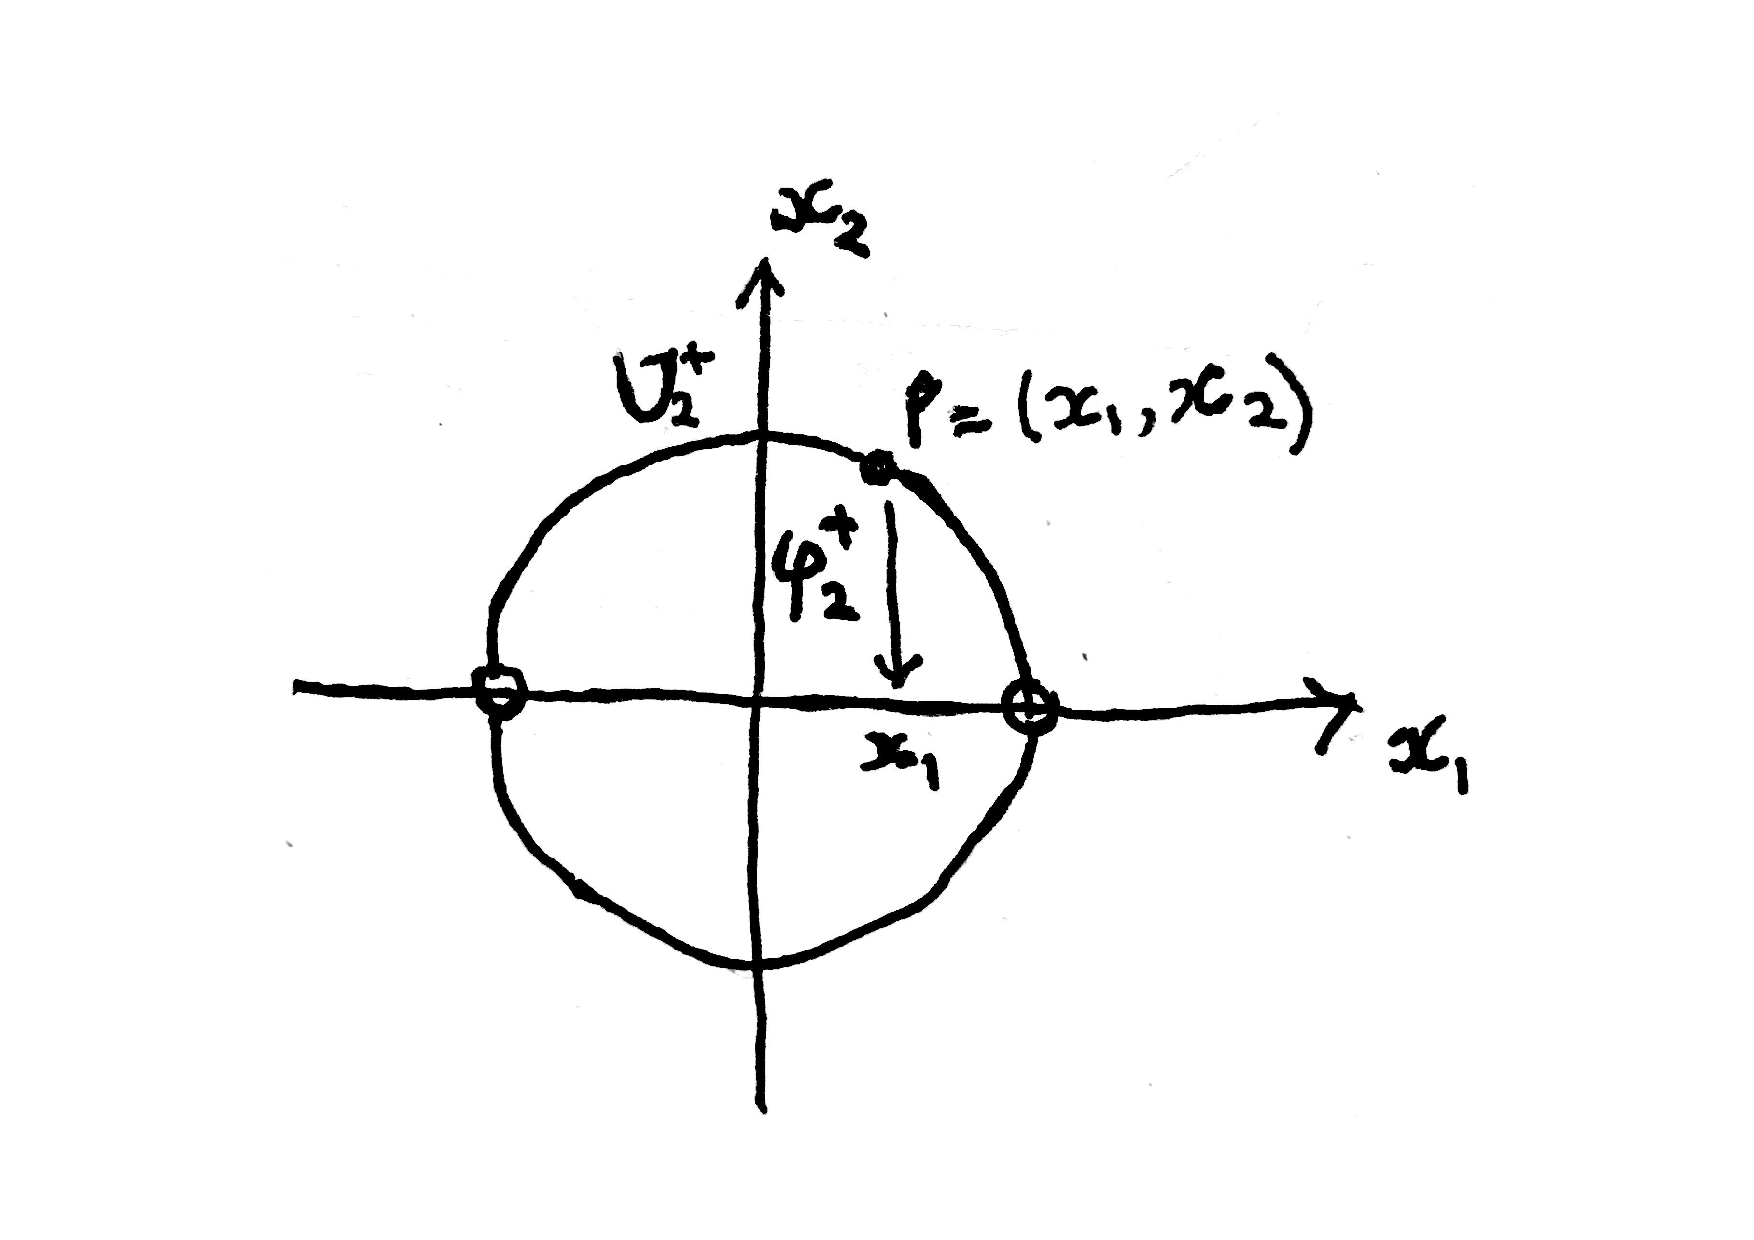
\includegraphics[keepaspectratio, scale=0.2]{localCoSysOfS1_2.pdf}
        \caption{$S^1$の局所座標系}
        \label{}
      \end{minipage}
      %---- 図はここまで ----------------------
    \end{tabular}
  \end{figure}
\begin{definition}
    $\{(U_\alpha ,\varphi _\alpha)\}_{\alpha \in A}$
    を$m$次元$C^r$級多様体$M$の$1$つの$m$次元$C^r$級
    座標近傍とする. $M$の開集合$V$と$V$から$\mathbb{R}^m$
    への写像$\psi$の対$(V,\psi)$が次の条件(1), (2)
    を満たしているとき, $(V,\psi)$は
    $\{(U_\alpha ,\varphi _\alpha)\}_{\alpha \in A}$
    と両立するという. 
    \begin{itemize}
        \item[(1)]$\psi:V\to \mathbb{R}^m$の像
        $\psi (V)$は$\mathbb{R}^m$の開集合で
        $\psi$は$V$から$\psi (V)$への同相写像
        である. 
        \item[(2)] $V\cap U_\alpha \neq \phi$
        となる$\alpha$に対しては, 
        $\psi \circ \varphi_\alpha ^{-1}:
        \varphi_\alpha(V\cap U_\alpha)\to
        \psi(V\cap U_\alpha)$は$C^r$級微分同相
        写像である. 
    \end{itemize}
\begin{proposition}
    $(V_1,\psi_1)$, $(V_2,\psi_2)$がともに与えられた
    座標近傍系$\{(U_\alpha ,
    \varphi _\alpha)\}_{\alpha \in A}$
    と両立していて, $V_1\cap V_2\neq \phi$
    とすると, $\psi_2\circ \psi_1^{-1}$は$C^r$級
    写像となる. 
\end{proposition}
\begin{proof}
    任意の点$x\in V_1\cap V_2$に対し, 
    $x_\in U_\alpha$となる$(U_\alpha, 
    \varphi_\alpha)$が座票近傍系の中に
    存在する. 
    $$\psi_2\circ \psi_1^{-1}:
    \psi_1(V_1\cap V_2\cap U_\alpha)\to
    \psi_2(V_1\cap V_2\cap U_\alpha)$$
    は$(\psi_2\circ \varphi_\alpha^{-1})\circ
    (\psi_1\circ \varphi_\alpha^{-1})^{-1}$
    と分解され, 
    $(\psi_2\circ \varphi_\alpha^{-1})$, 
    $(\psi_1\circ \varphi_\alpha^{-1})^{-1}$
    はそれぞれ$x\in V_1\cap V_2$
    に関して$C^r$級微分同相であるから, 
    $\psi_2\circ \psi_1^{-1}$も
    $x$に関して$C^r$級微分同相である. いま, 
    $x\in V_1\cap V_2$は任意であったから, 
    $\psi_2\circ \psi_1^{-1}$は$C^r$級
    微分同相写像である. 
\end{proof}
\begin{corollary}
    $(V,\psi)$が
    $C^r$級座標近傍系
    $\mathcal{S}=
    \{(U_\alpha, \varphi_\alpha)\}_{\alpha\in A}$
    と両立するとき, $\mathcal{S}\cup (V,\psi)$も
    $C^r$級座標近傍系になる. 
\end{corollary}
\begin{definition}
    位相空間$M$上に$C^r$級座標近傍系
    $\mathcal{S}=
    \{(U_\alpha, \varphi_\alpha)\}_{\alpha\in A}$
    が与えられているとする. 
    $\mathcal{S}$
    と両立する$(V,\psi)$の全体集合
    $\mathcal{M}=\mathcal{M}(\mathcal{S})$を
    $M$上の極大な$C^r$級座標近傍系とする. 
    ここで, 極大とは$\mathcal{M}$と両立する
    全ての$(U,\varphi)$が$\mathcal{M}
    =\mathcal{M}(\mathcal{S})$
    に属することをいう. この$\mathcal{M}
    =\mathcal{M}(\mathcal{S})$
    のことを$\mathcal{S}$から決まる
    $M$の$C^r$級極大座標近傍系という. 
\end{definition}
以降, $C^r$級多様体$M$が$C^r$級座標近傍系
$\mathcal{S}$によって定義されたとき, $M$には
$\mathcal{S}$から決まる$C^r$級極大座標近傍系
$\mathcal{M}(\mathcal{S})$を与え, 
$(M,\mathcal{M}(\mathcal{S}))$を
考えるものとする. 
\end{definition}

\subsection{$C^s$級写像}
$M$, $N$を$m$次元, $n$次元の$C^r$級多様体とし, 
$f$を連続写像とする. 
\begin{definition}\label{def:local coordinate display}
$M$, $N$の$C^r$級
座標近傍$(U,\varphi)$, 
$(V,\psi)$が存在し, 
$$f(U)\subset V$$
が成り立つ. 
$U$と$V$の中には座標近傍系$(x_1,\cdots x_m)$, 
$(y_1,\cdots y_n)$があるから, 
$f|U:U\to V$を
$$(y_1,\cdots y_n)=
f(x_1,\cdots x_m)$$
と表示することができる. この表示
を$(U;x_1,\cdots x_m)$と$(V;y_1,\cdots y_n)$
に関する$f$の局所座標表示という. 
\end{definition}
$f$の局所座標表示は本来, $U$, $V$の局所座標系
$\varphi=(x_1,\cdots ,x_m)$, 
$\psi=(y_1,\cdots ,y_n)$を用いて, 
$(y_1,\cdots y_n)=
\psi \circ f\circ \varphi^{-1}(x_1,\cdots x_m)$
と書くべきものであるので, 必要に応じてこちらの表記
を使うこととする. 
\begin{definition}\label{def:C^s map}
    連続写像$f:M\to N$が$1$点$p\in M$において
    $C^s$級であるとは, $p$を含む$M$の$C^r$級
    座標近傍$(U;x_1,\cdots x_m)$と
    $f(p)$を含む$N$の
    座標近傍$(V;y_1,\cdots y_n)$が存在して, 
    \begin{itemize}
        \item[(1)]$f(U)\subset V$
        \item[(2)]$(U;x_1,\cdots x_m)$と
        $(V;y_1,\cdots y_n)$に関する$f$の
        局所座標表示が$C^s$級である.
        (ただし, $0\leq s \leq r \leq \infty$) 
    \end{itemize}
    この$2$つの条件が成り立つことである. 
    $f$が任意の点$p\in M$で$C^s$級であるとき, 
    $f$は$C^s$級写像であるという. 
\end{definition}

\begin{proposition}
    連続写像$f:M\to N$が$1$点$p\in M$において
    $C^s$級であるという性質は, $p$, $f(p)$を
    それぞれ含む$C^r$級座標近傍$(U,\varphi)$, 
    $(V, \psi)$の選び方によらない. 
    (ただし, $0\leq s \leq r \leq \infty$)
\end{proposition}
\begin{proof}
    $f$は$p\in M$において$(U,\varphi)$, 
    $(V, \psi)$に関して$C^s$級であると仮定する. 
    $f(U')\subset V'$, $U'=U$, $V'=V$となるような
    $p$, $f(p)$をそれぞれ含む別の$C^r$級座標近傍
    $(U',\varphi')$, $(V, \psi')$をとると, 
    $\psi'\circ f\circ \varphi'^{-1}$は
    $$\psi'\circ f\circ \varphi'^{-1}=
    (\psi'\circ \psi^{-1})\circ
    (\psi \circ f\circ \varphi^{-1})\circ
    (\varphi \circ \varphi')$$
    と分解される. $\psi'\circ \psi^{-1}$, 
    $\varphi \circ \varphi'$はそれぞれ$M$, $N$
    における座標変換であるから$C^r$級であり, 
    $\psi \circ f\circ \varphi^{-1}$は
    仮定より$C^s$級であるから, 
    $\psi'\circ f\circ \varphi'^{-1}$は
    $C^s$級である. よって命題は証明された. 
\end{proof}
\begin{proposition}
    $M$, $N$, $Q$を$C^r$級多様体とする. 
    $f:M\to N$, $g:N\to Q$がともに$C^s$級
    写像なら, 合成写像$g\circ f:M\to Q$
    も$C^s$級である. 
    (ただし, $0\leq s \leq r \leq \infty$)
\end{proposition}
\begin{proof}
    \begin{itemize}
        \item[(1)]
        $p$を$M$の任意の点とすると, $g$は$C^s$
        級写像より, $g(V)\subset W$となうような
        $f(p)$, $g(f(p))$を含む座標近傍
        $(V,\psi)$, $(W, \omega)$が存在する. 
        また, $f$は$C^s$
        級写像より, $f(U)\subset V$となうような
        $p$を含む座標近傍$(U,\varphi)$が存在する. 
        よって, 任意の点$p\in M$において
        $g\circ f(p)\subset W$となるような
        $p$, $g\circ f(p)$を含む座標近傍
        $(U,\varphi)$, $(W, \omega)$の存在を
        示せた. 
        \item[(2)] 
        $\omega \circ (g\circ f)\circ \varphi^{-1}$
        は
        $$\omega \circ (g\circ f)\circ \varphi^{-1}
        =(\omega \circ g\circ \psi^{-1})\circ
        (\psi \circ f\circ \varphi^{-1})$$
        と分解される. 
        $g$は$C^s$級写像より, 
        $\omega \circ g\circ \psi^{-1}$
        は$C^s$級, 
        $f$は$C^s$級写像より,
        $\psi \circ f\circ \varphi^{-1}$
        は$C^s$級であるから, 
        $\omega \circ (g\circ f)\circ \varphi^{-1}$
        は$C^s$級となる. 
    \end{itemize}
    以上より, 合成写像$g\circ f:M\to Q$
    は$C^s$級である.
\end{proof}
\begin{definition}\label{def:C^s deffeomorphism}
    $M$, $N$を$C^r$級多様体とする. $f:M\to N$
    が$C^s$級微分同相写像であるとは, 次の条件
    (1), (2)を満たすことをいう. 
    \begin{itemize}
        \item[(1)]
        $f:M\to N$は全単射($1$対$1$かつ上への写像)
        である. 
        \item[(2)] 
        $f:M\to N$と$f^{-1}:N\to M$はともに$C^s$
        級写像である. 
    \end{itemize}
\end{definition}
\begin{proposition}\label{prop: cord-nabor condition}
    $M$を$m$次元$C^r$級多様体, $V$を$M$の開集合, 
    $V'$を$\mathbb{R}^m$の開集合とする. また, 
    $\varphi:V\to V'$を同相写像とする. 
    このとき, $(V,\varphi)$が$M$の$C^r$級
    座標近傍になるための必要十分条件は, 
    $\varphi:V\to V'$が, $C^r$級微分同相写像
    であることである. 
\end{proposition}
\begin{proof}
    まず, $(V,\varphi)$が$C^r$級座標近傍なら, 
    $\varphi:V\to V'$が, $C^r$級微分同相写像
    であることを証明する. 
    いま, $\varphi$は同相写像より, 全単射
    であることは明らかである. 
    $\varphi:V\to V'$の局所座標表示
    $\varphi \circ\varphi^{-1}:V'\to V'$と
    その逆写像が$C^r$級であることを示せばよいが, 
    逆写像も
    $\varphi \circ\varphi^{-1}:V'\to V'$
    となるため, 
    $\varphi \circ\varphi^{-1}:V'\to V'$
    が$C^r$級であることを示せばよい. これは
    恒等写像であるため, 明らかに$C^r$級である. 

    次に, $\varphi:V\to V'$が$C^r$級同相写像
    であると仮定して, $(V,\varphi)$が$M$の$C^r$級
    座標近傍になることを証明する. 
    $\mathcal{S}=\{(U_\alpha,
    \varphi_\alpha)\}_{\alpha\in A}$を
    $M$の$C^r$級座標近傍系とする. 上で証明した
    ように, $\varphi:U_\alpha\to U'_\alpha$
    は$C^r$級微分同相写像である. 
    $(V,\varphi)$から, $(U_\alpha,
    \varphi_\alpha)$への座標変換は, 
    $$\varphi_\alpha \circ \varphi^{-1}:
    \varphi(V\cap U_\alpha)\to 
    \varphi_\alpha(V\cap U_\alpha)$$
    $$\varphi \circ \varphi_\alpha^{-1}:
    \varphi_\alpha(V\cap U_\alpha)\to 
    \varphi(V\cap U_\alpha)$$
    であって, これらは$C^r$級微分同相写像
    の合成になっているから, $C^r$級である. 

    よって, $(V,\varphi)$は$\mathcal{S}$で決まる
    極大$C^r$級座標近傍系$\mathcal{M}(\mathcal{S})$
    に属することになり, $M$の$C^r$級座標近傍
    である. 
\end{proof}
%
\newpage
\section{接ベクトル空間}
\subsection{接ベクトル空間}
$M$を$m$次元$C^r$級多様体とし 
($1\leq r\leq \infty$), $M$の$1$点$p$を通る
$C^r$級曲線$c$を考える. ここで, $c$のパラメータ
$t$は$-\epsilon \leq t\leq \epsilon$の
範囲を動くとし, $c(0)=p$であるとする. 
\begin{definition}\label{def:directional derivative}
    点$p$における方向微分$\boldsymbol{v}$とは, 
    点$p$の開近傍上で
    定義された$C^r$級関数$f$に実数
    $\boldsymbol{v}(f)$を
    対応させる操作であって, 次の性質(0), (1), (2)
    をもつものである. 
    \begin{itemize}
        \item[(0)]$f$と$g$が点$p$の十分
        小さな近傍で上で一致すれば, 
        $\boldsymbol{v}(f)=\boldsymbol{v}(g)$. 
        \item[(1)]$\boldsymbol{v}(af+bg)
        =a\boldsymbol{v}(f)+
        a\boldsymbol{v}(g)$($a,b\in \mathbb{R}$)
        \item[(2)]$\boldsymbol{v}(fg)=
        \boldsymbol{v}(f)g(p)+
        \boldsymbol{v}(g)f(p)$
    \end{itemize}
\end{definition}
    \begin{example}
        $c$に沿う($t=0$における)方向微分
        点$p\in M$の開近傍$U$で定義された任意の
        $C^r$級関数$f$を考える. 
        $c:(-\epsilon, \epsilon)\to U$
        と$f:U\to \mathbb{R}$の合成関数
        $f(c(t))$の$t=0$における
        通常の微分係数
        $$\left .\frac{df(c(t))}{dt}\right|_{t=0}
        \ \left( \lim_{t\to 0}
        \frac{f(c(t))-f(c(0))}{t} \right) $$
        を考える. 
        関数$f$に上の微分係数を対応させる対応
        $$\left .\frac{dc}{dt}\right|_{t=0}:
        f\mapsto 
        \left .\frac{df(c(t))}{dt}\right|_{t=0}$$
        を曲線$c$の$t=0$における速度ベクトルという. 
        曲線$c$の$t=0$における速度ベクトルは
        方向微分である. 実際, 
        \begin{itemize}
            \item[(0)]$f$, $g$が点$p$の開近傍上で定義
            された$C^r$級関数で, $p$のある十分
            小さな開近傍上で$f=g$ならば, 
            $$\left .\frac{dc}{dt}\right|_{t=0}
            (f)=\left .\frac{df(c(t))}{dt}\right|_{t=0}=
            \left .\frac{dg(c(t))}{dt}\right|_{t=0}=
            \left .\frac{dc}{dt}\right|_{t=0}(g)$$
            \item[(1)]$f$, $g$が点$p$の開近傍上で定義
            された$C^r$級関数で, $a, b\in \mathbb{R}$
            のとき, 
            \begin{eqnarray*}
                \left .\frac{dc}{dt}\right|_{t=0}
            (af+bg)&=&
            \left .\frac{d(af(c(t))+bg(c(t)))}{dt}
            \right|_{t=0}\\
            &=&
            a\left .\frac{df(c(t))}{dt}\right|_{t=0}+
            b\left .\frac{dg(c(t))}{dt}\right|_{t=0}\\
            &=&
            a\left .\frac{dc}{dt}\right|_{t=0}(f)+
            b\left .\frac{dc}{dt}\right|_{t=0}(g)
            \end{eqnarray*}
            \item[(2)]
            $f$, $g$が点$p$の開近傍上で定義
            された$C^r$級関数で, $fg$をそれらの
            積とすれば, 
            \begin{eqnarray*}
                \left .\frac{dc}{dt}\right|_{t=0}
            (fg)&=&
            \left\{\frac{df(c(t))}{dt}g(c(t))+
            f(c(t))\frac{dg(c(t))}{dt}
            \right\}_{t=0}\\
            &=&
            \left .\frac{df(c(t))}{dt}\right|_{t=0}
            g(p)+ f(p)
            \left .\frac{dg(c(t))}{dt}\right|_{t=0}\\
            &=&
            \left .\frac{dc}{dt}\right|_{t=0}(f)g(p)
            +f(p)
            \left .\frac{dc}{dt}\right|_{t=0}(g)
            \end{eqnarray*}
        \end{itemize}
    \end{example}
    \begin{example}
        $p$を含む座標近傍$(U;x_1,\cdots x_m)$を
        $1$つ固定する. $p$のまわりで定義された
        $C^r$級関数$f$に, $p$における$x_i$
        方向の偏微分係数を対応させる操作を
        $\left(\frac{\partial}{\partial x_i}
        \right)_p$と書く. すなわち, 
        $$\left(\frac{\partial}{\partial x_i}
        \right)_p:f\mapsto 
        \frac{\partial f}{\partial x_i}(p)$$
        である.  
        このとき, $\left(\frac{\partial}
        {\partial x_i}\right)_p$は$p$における
        方向微分の性質(0), (1), (2)を満たす. 
    \end{example}
    \begin{definition}
        点$p\in M$における方向微分全ての集合を
        $$D_p^r(M)$$
        と表す. $D_p^r(M)$の$2$元$u$, $v$と
        実数$a$に対して, 
        和$\boldsymbol{u}+\boldsymbol{v}$と
        実数倍$a\boldsymbol{u}$を
        $$(\boldsymbol{u}+\boldsymbol{v})(f)=
        \boldsymbol{u}(f)+\boldsymbol{v}(v)$$
        $$a\boldsymbol{u}(f)=
        a(\boldsymbol{u}(f))$$
        と定めると, $D_p^r(M)$は
        $\mathbb{R}$上のベクトル空間となる. 
        ただし, $D_p^r(M)$のゼロベクトルは
        任意の$f$に$0$を対応させる自明な
        方向微分$\boldsymbol{0}$である. 
    \end{definition}
    \begin{proposition}
        ベクトル空間$D_p^r(M)$の元として, 
        $m$個のベクトル
        $\left(\frac{\partial}{\partial x_1}\right)_p, 
        \cdots 
        \left(\frac{\partial}{\partial x_m}\right)_p$
        は$1$次独立である. 
    \end{proposition}
    \begin{proof}
        実数$a_1,\cdots a_m$に対して
        $a_1\left(\frac{\partial}{\partial x_1}\right)_p+
        \cdots +
        a_m\left(\frac{\partial}{\partial x_m}\right)_p=
        \boldsymbol{0}$
        ならば, $a_1=\cdots =a_m=0$であることを
        示せばよい. 
        $a_1\left(\frac{\partial}{\partial x_1}\right)_p+
        \cdots +
        a_m\left(\frac{\partial}{\partial x_m}\right)_p=
        \boldsymbol{0}$
        と仮定すると, 点$p$のまわりで定義された
        任意の$C^r$級関数$f$について
        $a_1\left(\frac{\partial}{\partial x_1}\right)_p(f)+
        \cdots +
        a_m\left(\frac{\partial}{\partial x_m}\right)_p(f)=
        0$
        が成り立つ. つまり, 
        $a_1\frac{\partial f}{\partial x_1}(p)+
        \cdots +
        a_m\frac{\partial f}{\partial x_m}(p)=
        0$
        となる. $f$は任意であったから, $f=x_1$
        という関数をとってくると, 
        \begin{eqnarray*}
            \frac{\partial f}{\partial x_1}&=&1\\
            \frac{\partial f}{\partial x_i}&=&0
            \ \text{($i\geq 2$)}
        \end{eqnarray*}
        であるから, 最初の項のみが$a_1$となって残り, 
        あとは消える. よって$a_1=0$がわかる. 
        同様に$f=x_2,\cdots x_m$を次々に代入
        して, $a_1=\cdots =a_m=0$が示される. 
        これで命題が証明された. 
    \end{proof}
    \begin{definition}\label{def:tangent vector space}
        $m$個のベクトル
        $\left(\frac{\partial}{\partial x_1}\right)_p, 
        \cdots 
        \left(\frac{\partial}{\partial x_m}\right)_p$
        の張る$D_p^r(M)$の部分ベクトル空間を, 点$p$
        における$M$の接ベクトル空間とよび, 
        $$T_p(M)$$
        という記号で表す. 接ベクトル空間$T_p(M)$の
        元を接ベクトルとよぶ. 
    \end{definition}
    \begin{figure}[H]
        \centering
        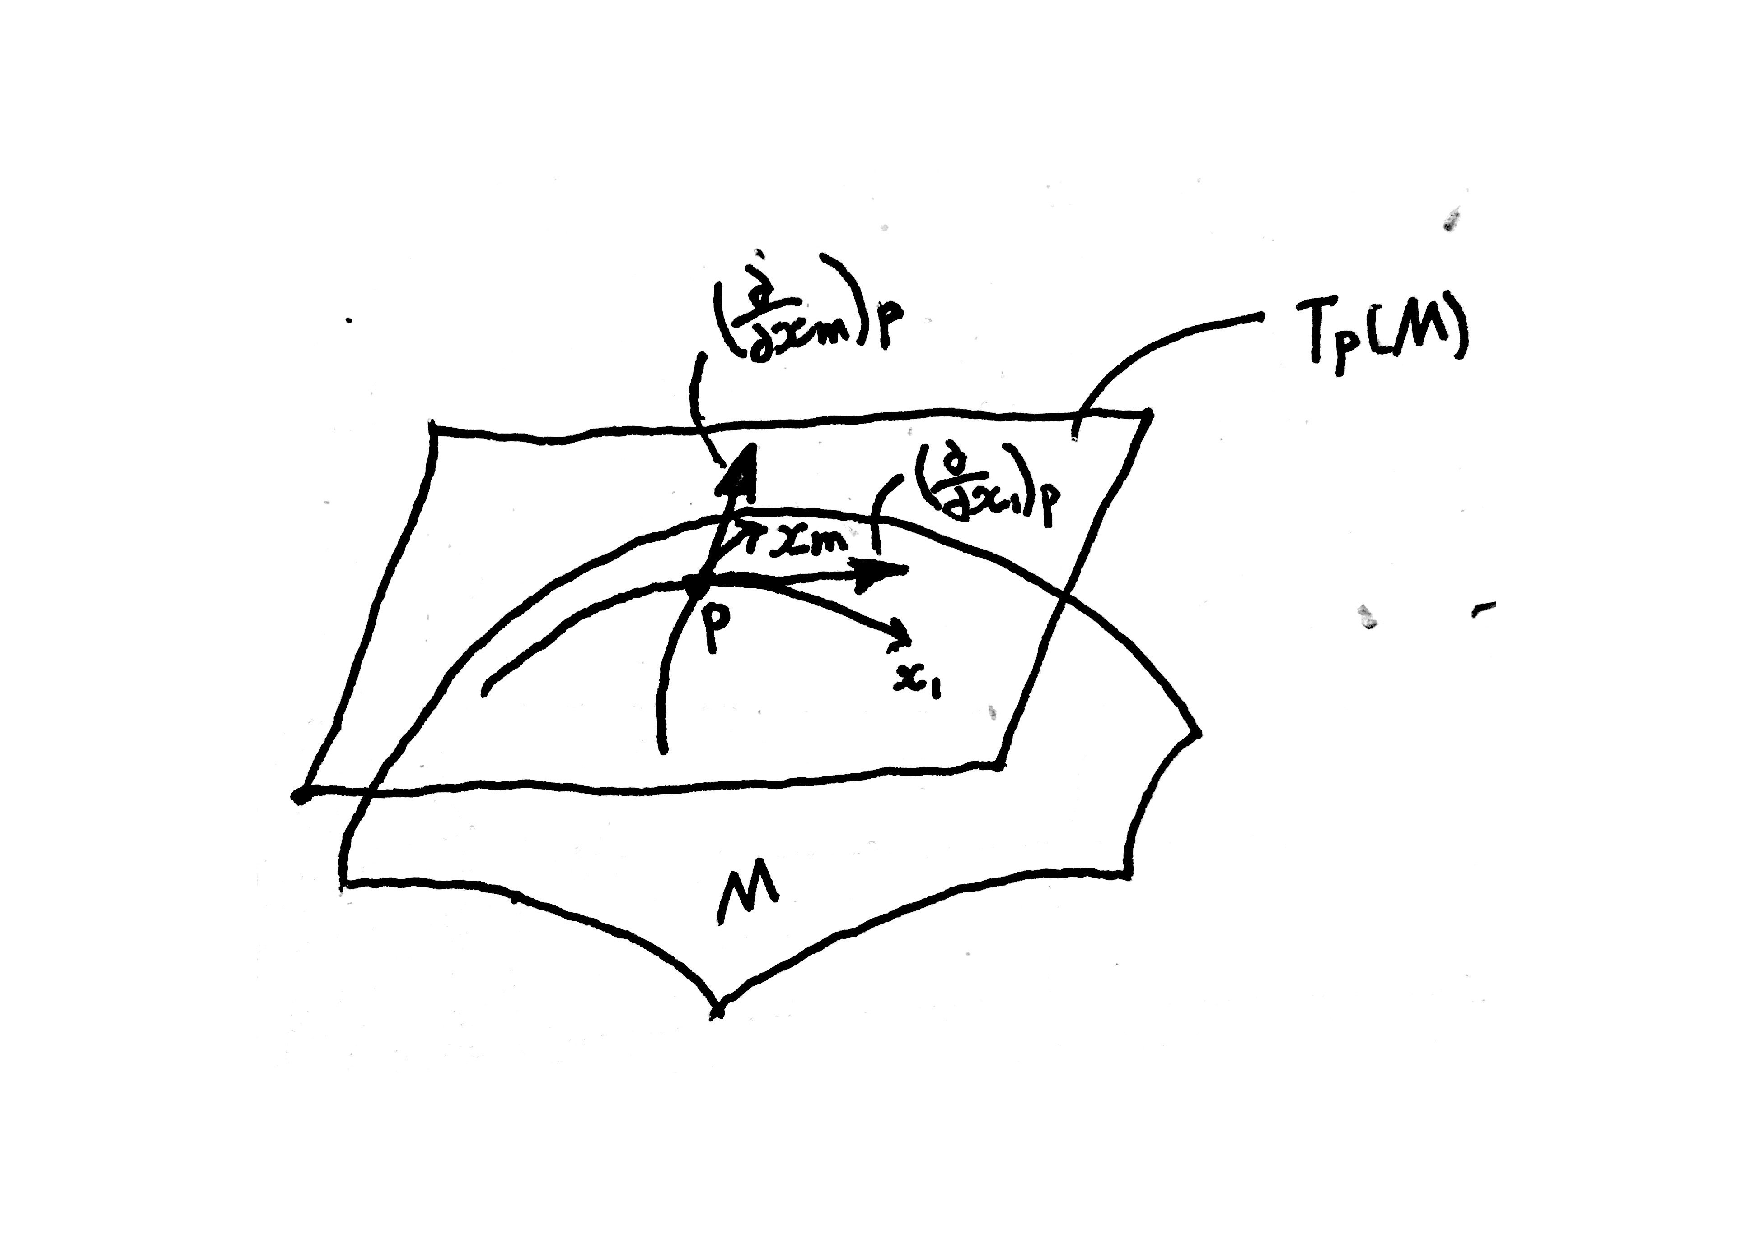
\includegraphics[keepaspectratio, scale=0.4]{tangentVectorSpace_2.pdf}
        \caption{接ベクトル空間$T_p(M)$}
        \label{tangentVectorSpace}
       \end{figure}
       
    \begin{proposition}
        $T_p(M)$は点$p$のまわりの局所座標系のとり方に
        よらず一意に定まる. つまり, 点$p$のまわりで
        $(x_1,\cdots ,x_m)$と別の局所座標系
        $(y_1,\cdots ,y_m)$を選んだとき, 
        方向微分
        $$\left(\frac{\partial}{\partial y_1}\right)_p, 
        \cdots ,
        \left(\frac{\partial}{\partial y_m}\right)_p$$
        の張る$D_p^r(M)$の部分ベクトル空間は, 
        $$\left(\frac{\partial}{\partial x_1}\right)_p, 
        \cdots ,
        \left(\frac{\partial}{\partial x_m}\right)_p$$
        の張る部分ベクトル空間に一致する. 
    \end{proposition}
    \begin{proof}
        点$p$のまわりで定義された任意の$C^r$級
        関数$f$について, 次の変換公式が成り立つ. 
        $$\frac{\partial f}{\partial x_i}
        =\sum_{j=1}^{m}\frac{\partial y_j}
        {\partial x_i}(p)
        \frac{\partial f}{\partial y_j}(p).$$
        方向微分の記号を使ってかくと, 
        $$\left(\frac{\partial}{\partial x_i}\right)_p=
        \sum_{j=1}^{m}
        \frac{\partial y_j}{\partial x_i}(p)
        \left(\frac{\partial}{\partial y_j}\right)_p$$
        を得る. 右辺の
        $\frac{\partial y_j}{\partial x_i}(p)$
        を単なる実数と思うと, この式は, 
        方向微分$\left(\frac{\partial}{\partial x_i}\right)_p$
        ($i=1,\cdots m$)が
        $\left(\frac{\partial}{\partial y_1}\right)_p, \cdots 
        ,\left(\frac{\partial}{\partial y_m}\right)_p$
        の$1$次結合で表されるということを意味している. 
        したがって, 
        $\left(\frac{\partial}{\partial x_1}\right)_p, \cdots 
        ,\left(\frac{\partial}{\partial x_m}\right)_p$
        は
        $\left(\frac{\partial}{\partial y_1}\right)_p, \cdots 
        ,\left(\frac{\partial}{\partial y_m}\right)_p$
        の張るベクトル空間に属している. 
        $(x_1,\cdots ,x_m)$と$(y_1,\cdots ,y_m)$
        の役割を入れ換えて同じ議論をすれば, 逆に
        $\left(\frac{\partial}{\partial y_1}\right)_p, \cdots 
        ,\left(\frac{\partial}{\partial y_m}\right)_p$
        が
        $\left(\frac{\partial}{\partial x_1}\right)_p, \cdots 
        ,\left(\frac{\partial}{\partial x_m}\right)_p$
        の張るベクトル空間に属していることも証明される. 
        したがって, 両者の張るベクトル空間は一致する. 
    \end{proof}
    上の証明中に出てきた基底の変換公式は重要であるから
    改めて命題の形で述べておく. 
    \begin{proposition}\label{prop:basis conversion}
        点$p$のまわりに$2$つの局所座標系
        $(x_1,\cdots x_m)$, $(y_1,\cdots ,y_m)$
        があると, それに応じて$T_p(M)$の基底
        $$\left<\left(\frac{\partial}
        {\partial x_1}\right)_p,\cdots ,
        \left(\frac{\partial}
        {\partial x_m}\right)_p\right>,\ 
        \left<d\left(\frac{\partial}
        {\partial y_1}\right)_p,\cdots ,
        \left(\frac{\partial}
        {\partial y_m}\right)_p\right>$$
        が定まる. それらの間には次の関係式
        が成り立つ. 
        $$\left(\frac{\partial}{\partial x_i}\right)_p=
        \sum_{j=1}^{m}
        \frac{\partial y_j}{\partial x_i}(p)
        \left(\frac{\partial}{\partial y_j}\right)_p$$
    \end{proposition}
    \begin{proposition}\label{prop:dc/dt is tangent vector}
        曲線$c$の$t=0$における速度ベクトル
        $\left .\frac{dc}{dt}\right|_{t=0}$
        は$T_p(M)$の元, すなわち接ベクトルである. 
    \end{proposition}
    \begin{proof}
        点$p$のまわりの局所座標系$(x_1,\cdots ,x_m)$
        を任意に固定する. 
        $\left .\frac{dc}{dt}\right|_{t=0}$
        が$\left(\frac{\partial}{\partial x_1}\right), 
        \cdots ,
        \left(\frac{\partial}{\partial x_m}\right)$
        という形の方向微分の$1$次結合として表されている
        ことを証明すればよい. 
        $p$のまわりで定義された任意の$C^r$級関数$f$を
        をとり, 関数$f$と曲線$c$を局所座標表示したものが
        それぞれ, 
        $$f(x_1,\cdots ,x_m),\ 
        c(t)=(x_1(t),\cdots x_m(t))$$
        であったとすると, 
        \begin{eqnarray*}
            \left .\frac{dc}{dt}\right|_{t=0}(f)&=&
            \left .\frac{d}{dt}f(x_1(t),\cdots ,x_m(t))
            \right|_{t=0}\\
            &=&\sum_{i=1}^{m}\frac{dx_i}{dt}(0)
            \frac{\partial f}{\partial x_i}(p)
        \end{eqnarray*}
        と計算される(合成関数の微分法). 
        $f$は任意であったから, 方向微分としての等式
        $$\left .\frac{dc}{dt}\right|_{t=0}=
        \sum_{i=1}^{m}\frac{dx_i}{dt}(0)
            \left(\frac{\partial}{\partial x_i}
            \right)_p$$
        を得る. 右辺の$\frac{dx_1}{dt}(0), 
        \cdots ,\frac{dx_m}{dt}(0)$
        を単なる実数と思うと, 
        $\left .\frac{dc}{dt}\right|_{t=0}$
        が
        $\left(\frac{\partial}{\partial x_1}\right), 
        \cdots ,
        \left(\frac{\partial}{\partial x_m}\right)$
        の$1$次結合で表されることがわかる. 
        これで命題が証明された. 
    \end{proof}

\subsection{$C^r$級写像の微分}
$M$, $N$をそれぞれ$m$次元, $n$次元の$C^r$級
多様体, $f:M\to N$を
$C^r$級写像とし($1 \leq r\leq \infty$), 
点$p\in M$を通る$M$上の$C^r$曲線を
$$c:(-\epsilon, \epsilon)\to M,\ c(0)=p$$
とする. この曲線を写像$f$でうつすと, 点
$q=f(p)$を通る$N$上の$C^r$曲線
$$f\circ c:(-\epsilon, \epsilon)\to N, f^\circ c(0)=q$$
が得られる. 
\begin{figure}[H]
    \centering
    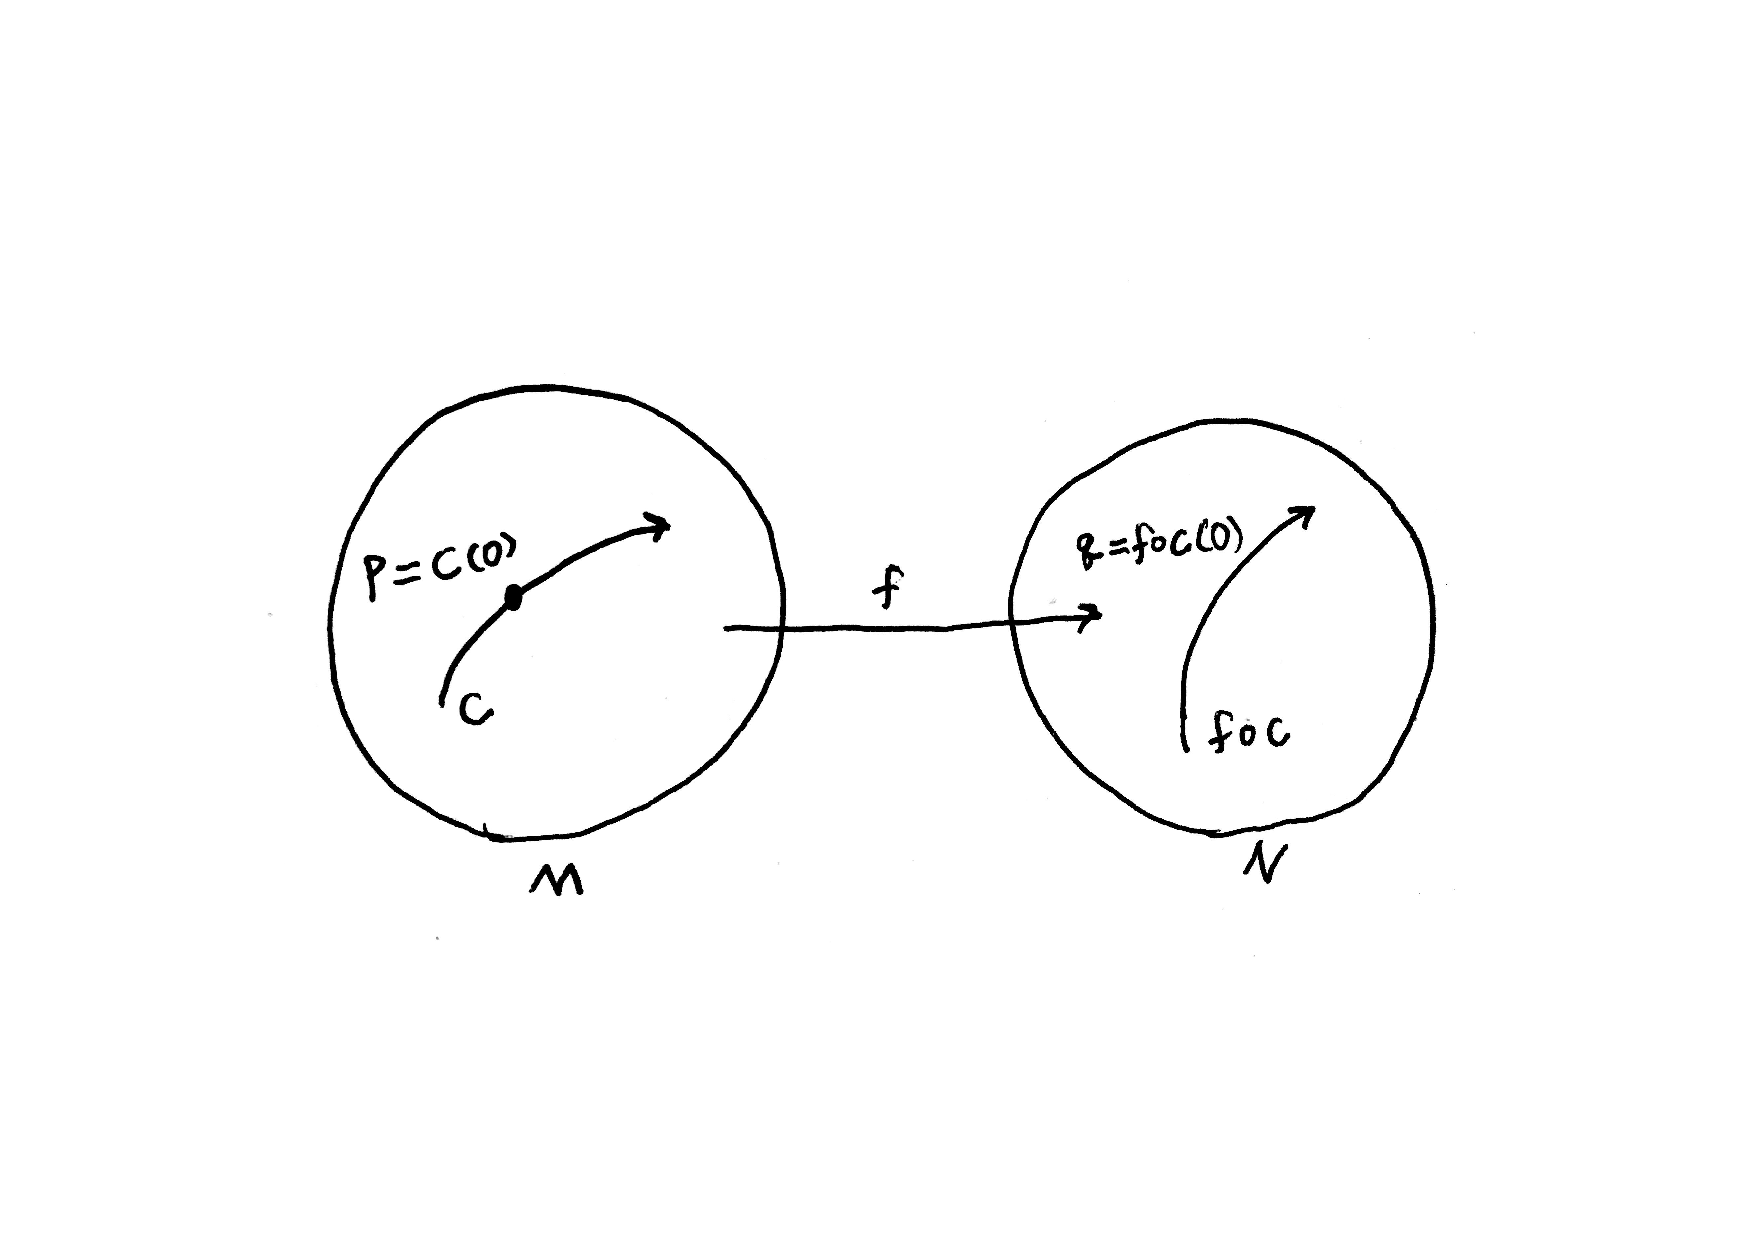
\includegraphics[keepaspectratio, scale=0.4]{cTofc.pdf}
    \caption{$C^r$曲線$c$, $f\circ c$}
    \label{cTofc}
   \end{figure}
   
$t=0$における曲線$c$の速度ベクトル
$$\left .\frac{dc}{dt}\right|_{t=0}\in T_p(M)$$
と, $t=0$における曲線$f\circ c$の速度ベクトル
$$\left .\frac{d(f\circ c)}{dt}\right|_{t=0}
\in T_q(M)$$
の関係を調べる. 
\begin{proposition}\label{prop:relation of v and w}
    $t=0$における$c$と$f\circ c$の速度ベクトルを
    それぞれ
    $$\left .\frac{dc}{dt}\right|_{t=0}=
    \sum_{i=1}^{m}v_i\left(\frac{\partial}
    {\partial x_i}\right)_p,\ 
    \left .\frac{d(f\circ c)}{dt}\right|_{t=0}=
    \sum_{j=1}^{n}w_j\left(\frac{\partial}
    {\partial y_j}\right)_q$$
    とおくと, 係数$v_1,\cdots ,v_m$と
    $w_1,\cdots ,w_n$の間には次の関係がある. 
    $$w_j=\sum_{i=1}^{m}\frac{\partial f_j}
    {\partial x_i}(p)v_i\ (j=1,\cdots ,n)$$
    またこの式を, 縦ベクトルと行列を使って書くと
    $$\begin{pmatrix}
          w_1 \\
          \vdots \\
          w_n 
        \end{pmatrix}
        =
        \left(
        \begin{array}{ccc}
          \frac{\partial f_1}{\partial x_1}(p)&\cdots &\frac{\partial f_1}{\partial x_m}(p)\\
          \vdots &\ddots& \vdots \\
          \frac{\partial f_n}{\partial x_1}(p)&\cdots &\frac{\partial f_n}{\partial x_m}(p) 
        \end{array} 
        \right)
        \begin{pmatrix}
          v_1\\
          \vdots \\
          v_m
        \end{pmatrix}
        $$
    となる. 
\end{proposition}
\begin{proof}
    点$p$を含む$M$の座標近傍$(U;x_1,\cdots x_m)$
    と, $q=f(p)$を含む$N$の座標近傍
    $(V;y_1,\cdots y_n)$を$f(U)\subset V$
    となるようにとる. $f$を$(U;x_1,\cdots x_m)$
    と$(V;y_1,\cdots y_n)$に関して局所座標
    表示したものが
    \begin{eqnarray*}
        y_1&=&f_1(x_1,\cdots ,x_m)\\
        &\vdots& \\
        y_n&=&f_n(x_1,\cdots ,x_m)
    \end{eqnarray*}
    であるとする. 右辺の関数は$(x_1,\cdots x_m)$
    に関して$C^r$級である. 
    パラメータ$t$の動く範囲$-\epsilon\leq t \epsilon$
    を十分小さくとれば, 曲線$c$は
    $(U;x_1,\cdots x_m)$の中に含まれるとしてよい. 
    局所座標系$(x_1,\cdots ,x_m)$に関する$c$の
    局所座標表示を
    $$c(t)=(x_1(t),\cdots ,x_m(t))$$
    とすると, 曲線$f\circ c$の$(y_1,\cdots ,y_n)$
    に関する局所座標表示は
    \begin{eqnarray*}
        f\circ c(t)&=&(y_1(t),\cdots ,y_n(t))\\
        &=&(f_1(x_1(t),\cdots ,x_m(t)),\cdots ,
        f_n(x_1(t),\cdots ,x_m(t)))
    \end{eqnarray*}
    で与えられる. 
    曲線$c$の$t=0$における速度ベクトルを
    $$\left .\frac{dc}{dt}\right|_{t=0}=
    v_1\left(\frac{\partial}{\partial x_1}\right)_p
    +\cdots +
    v_m\left(\frac{\partial}{\partial x_m}\right)_p$$
    とおく. ただし$v_1,\cdots ,v_m$は実数である. 
    命題\ref{prop:dc/dt is tangent vector}より, 
    $v_i=\frac{dx_i}{dt}(0)\ (i=1,\cdots ,m)$
    である. 曲線$f\circ c$の速度ベクトルを求めると
    \begin{eqnarray*}
        \left .\frac{f\circ c}{dt}\right|_{t=0}
        &=&\sum_{j=1}^{n}\frac{dy_j}{dt}(0)
        \left(\frac{\partial}{\partial y_j}
        \right)_q\\
        &=&
        \sum_{j=1}^{n}\left .
        f_j(x_1(t),\cdots ,x_m(t))\right|_{t=0}
        \left(\frac{\partial}{\partial y_j}
        \right)_q\\
        &=&
        \sum_{j=1}^{n}\left\{
            \sum_{i=1}^{m}\frac{\partial f_j}
            {\partial x_i}(p)
            \frac{dx_i}{dt}(0)
        \right\}
        \left(\frac{\partial}{\partial y_j}
        \right)_q\\
        &=&
        \sum_{j=1}^{n}\left\{
            \sum_{i=1}^{m}\frac{\partial f_j}
            {\partial x_i}(p)
            v_i
        \right\}
        \left(\frac{\partial}{\partial y_j}
        \right)_q
    \end{eqnarray*}
    となる. 速度ベクトル
    $\left .\frac{f\circ c}{dt}\right|_{t=0}$
    の係数を$w_1, \cdots ,w_n$とすると, 
    $$w_j=\sum_{i=1}^{m}\frac{\partial f_j}
    {\partial x_i}(p)v_i\ (j=1,\cdots ,n)$$
    を得る. よって命題は証明された. 
\end{proof}
\begin{definition}\label{def:Jacobian matrix}
    命題\ref{prop:relation of v and w}
に現れた$n$行$m$列の行列
$$\left(
    \begin{array}{ccc}
      \frac{\partial f_1}{\partial x_1}(p)&\cdots &\frac{\partial f_1}{\partial x_m}(p)\\
      \vdots &\ddots& \vdots \\
      \frac{\partial f_n}{\partial x_1}(p)&\cdots &\frac{\partial f_n}{\partial x_m}(p) 
    \end{array} 
  \right)$$
を, 点$p$における写像$f:M\to N$のヤコビ行列
とよび, 記号で
$$(Jf)_p$$
と表す. ヤコビ行列$(Jf)_p$は, 局所座標系
$(x_1,\cdots ,x_m)$と$(y_1,\cdots ,y_n)$
を選ぶことによって決まる行列である. 
\end{definition}
命題\ref{prop:relation of v and w}より次の
系が分かる. 
\begin{corollary}\label{coro:any c is OK}
    $\left .\frac{d(f\circ c)}{dt}\right|_{t=0}$
    は$\left .\frac{dc}{dt}\right|_{t=0}$
    のみに依存して定まり, 点$p$から離れたところ
    での$c$の振る舞いによらない. 
    すなわち, 点$p\in M$を通る曲線$2$本を
    $$c:(-\epsilon, \epsilon)\to M\ (c(0)=p)$$
    $$c':(-\epsilon, \epsilon)\to M\ (c'(0)=p)$$
    とし, 
    $\left .\frac{dc}{dt}\right|_{t=0}=
    \left .\frac{dc'}{dt}\right|_{t=0}$
    と仮定すると, 
    $\left .\frac{d(f\circ c)}{dt}\right|_{t=0}=
    \left .\frac{d(f\circ c')}{dt}\right|_{t=0}$
    が成り立つ. なぜなら$f$を固定しておけば, 
    ベクトル$(w_1,\cdots ,w_n)$は, ベクトル
    $(v_1,\cdots ,v_m)$のみから計算
    されるからである. 
\end{corollary}
\begin{proposition}\label{prop:c exist}
    $T_p(M)_p$に属する任意のベクトル$\boldsymbol{v}$
    に対し, 点$p$を通る$C^r$級曲線
    $$c:(-\epsilon, \epsilon)\to M\ (c(0)=p)$$
    が存在して, $\left .\frac{dc}{dt}
    \right|_{t=0}=\boldsymbol{v}$
    が成り立つ. 
\end{proposition}
\begin{proof}
    $p$のまわりの局所座標系$(x_1,\cdots ,x_m)$
    を固定して考える. このとき, 
    $$\boldsymbol{v}=
    v_1\left(\frac{\partial}{\partial x_1}\right)_p
    +\cdots +
    v_m\left(\frac{\partial}{\partial x_m}\right)_p$$
    であるとする. これに応じて, 曲線$c$を
    $$c(t)=(a_1+v_1t,\cdots ,a_m+v_mt)$$
    と定義すればよい. ここに, $(a_1,\cdots ,a_m)$
    は$P$の局所座標である. 速度ベクトル
    $\left .\frac{dc}{dt}\right|_{t=0}$
    を計算すれば, $\boldsymbol{v}$に一致する
    ことが確かめられる. 
\end{proof}
系\ref{coro:any c is OK}と命題\ref{prop:c exist}
により, 次のような写像
$$T_p(M)\to T_q(N),\ 
\left .\frac{dc}{dt}\right|_{t=0}\mapsto
\left .\frac{d(f\circ c)}{dt}\right|_{t=0}
\ (q=f(p))$$
が自然に定義できる. 
\begin{definition}\label{def:differential}
    こうして得られた写像を
    $$(df)_p:T_p(M)\to T_q(N)$$
    と書き, 点$p$における$f:M\to N$
    の微分とよぶ. 
\end{definition}
\begin{figure}[H]
    \centering
    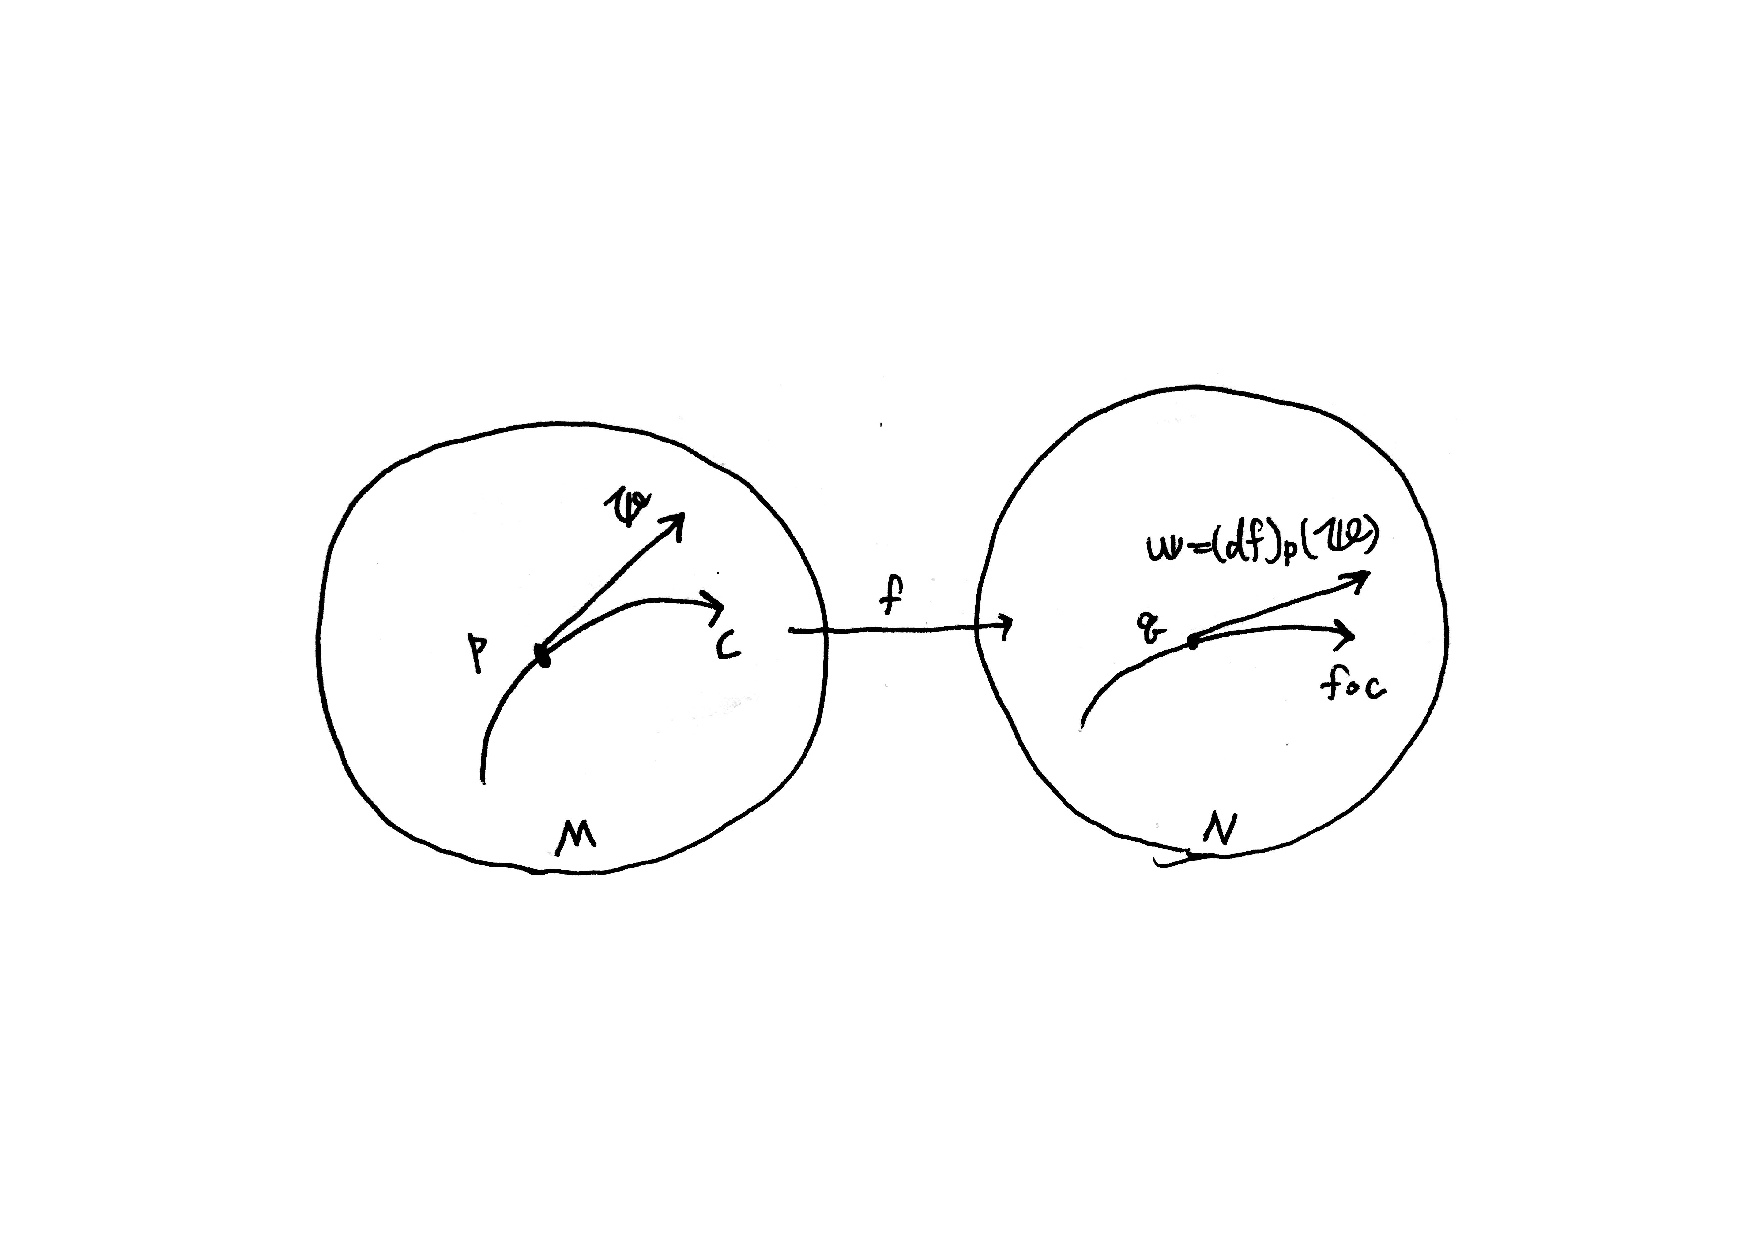
\includegraphics[keepaspectratio, scale=0.5]{differential.pdf}
    \caption{$f$の微分$(df)_p:T_p(M)\to T_q(N)$}
    \label{differential}
   \end{figure}
\begin{proposition}
    $(df)_p:T_p(M)\to T_p(M)$は線型写像である. 
\end{proposition}
\begin{proof}
    線型写像とはベクトルの和をベクトルの和にうつし, 
    ベクトルの$a$倍をベクトルの$a$倍にうつすような写像
    である. 
    $p$, $q$のまわりにそれぞれ局所座標系
    $(x_1,\cdots ,x_m)$, $(y_1,\cdots ,y_n)$
    をとり, $T_p(M)$, $T_q(N)$の中に
    基底$\left< \left(\frac{\partial}
    {\partial x_1}\right)_p,\cdots ,
    \left(\frac{\partial}
    {\partial x_m}\right)_p\right>$, 
    $\left< \left(\frac{\partial}
    {\partial y_1}\right)_p,\cdots ,
    \left(\frac{\partial}
    {\partial y_n}\right)_p\right>$
    を固定すると, 
    任意の$\boldsymbol{v}\in T_p(M)$は
    $$\boldsymbol{v}=
    \sum_{i=1}^{m}v_i
    \left(\frac{\partial}{\partial x_i}
    \right)_p$$
    と書け, 数ベクトル$(v_1,\cdots ,v_m)$
    と$1$対$1$に対応する. 同様に, 
    任意の$\boldsymbol{w}\in T_q(N)$は
    $$\boldsymbol{w}=
    \sum_{j=1}^{n}v_i
    \left(\frac{\partial}{\partial y_j}
    \right)_q$$
    と書け, 数ベクトル$(w_1,\cdots ,w_n)$
    と$1$対$1$に対応する. 今, 
    $\boldsymbol{w}=(df)_p(\boldsymbol{v})$
    であるとすると, 
    $\boldsymbol{w}$と$\boldsymbol{v}$
    に対応する数ベクトルを縦ベクトルに書いたとして, 
    $$\begin{pmatrix}
        w_1\\
        \vdots \\
        w_n
    \end{pmatrix}=(Jf)_p
    \begin{pmatrix}
        v_1\\
        \vdots \\
        v_m
    \end{pmatrix}$$
    の関係がある. $(Jf)_p$は点$p$における$f$
    のヤコビ行列である. この関係から
    $(df)_p:\boldsymbol{v}\mapsto 
    \boldsymbol{w}$が線型写像であることがわかる. 
\end{proof}
\begin{proposition}
    点$p$, $q$のまわりでそれぞれ局所座標系
    $(x_1,\cdots ,x_m)$, $(y_1,\cdots ,y_n)$
    を固定し, それによって$f$を
    \begin{eqnarray*}
        y_1&=&f_1(x_1,\cdots ,x_m)\\
        &\vdots&\\
        y_n&=&f_n(x_1,\cdots ,x_m)
    \end{eqnarray*}
    と局所座標表示する. このとき, 次の
    公式が成り立つ. 
    $$(df)_p\left( \left(
        \frac{\partial}{\partial x_i}
    \right)_p\right)=
    \sum_{j=1}^{n}\frac{\partial f_j}
    {\partial x_i}(p)\left(
        \frac{\partial}{\partial y_j}
    \right)_q$$
\end{proposition}
\begin{proof}
    $\left(\frac{\partial}{\partial x_i}\right)_p$
    を$\sum_{i=1}^{m}v_i\left(\frac
    {\partial}{\partial x_i}\right)_p$
    の形で表すと, $v_i=1,\ v_k=0\ (k\neq i)$
    である. 
    $(df)_p\left( \left(
        \frac{\partial}{\partial x_i}
    \right)_p\right)=
    \sum_{j=1}^{n}w_j\left(
        \frac{\partial}{\partial y_j}
    \right)_q$
    とおいたときの$w_j$は
    $$w_j=\sum_{i=1}^{m}v_i \frac{\partial f_j}
    {\partial x_i}(p)$$
    であるから, $v_i=1,\ v_k=0\ (k\neq i)$
    を代入して, 
    $$w_j=v_i \frac{\partial f_j}
    {\partial x_i}(p)$$
    を得る. よって, 
    $$(df)_p\left( \left(
        \frac{\partial}{\partial x_i}
    \right)_p\right)=
    \sum_{j=1}^{n}w_j\left(
        \frac{\partial}{\partial y_j}
    \right)_q=
    \sum_{j=1}^{n}\frac{\partial f_j}
    {\partial x_i}(p)\left(
        \frac{\partial}{\partial y_j}
    \right)_q$$
    が成り立つことが分かる. 
\end{proof}
\begin{proposition}
    $f:M\to N$を$C^r$級写像とする. $M$の点$p$
    における任意の接ベクトル$\boldsymbol{v}
    \in T_p(M)$と, $N$の点$f(p)$のまわりで定義された
    任意の$C^r$級関数$\xi$について
    $$((df)_p(\boldsymbol{v}))(\xi)=
    \boldsymbol{v}(\xi \circ f)$$
    が成り立つ. 
\end{proposition}
\begin{proof}
    $\boldsymbol{v}=\left .\frac{dc}{dt}
    \right|_{t=0}$であるような$C^r$級
    曲線$c:(-\epsilon, \epsilon)\to M$, 
    $c(0)=p$をとる. $(df)_p$の定義より, 
    $$(df)_p(\boldsymbol{v})=
    \left .\frac{d(f\circ c)}{dt}\right|_{t=0}$$
    である. 
    速度ベクトル$\left .\frac{d(f\circ c)}{dt}\right|_{t=0}$
    を方向微分と考えると, 
    $$\left .\frac{d(f\circ c)}{dt}\right|_{t=0}
    (\xi)=
    \left .\frac{d\xi(f\circ c(t))}
    {dt}\right|_{t=0}$$
    が成り立つ. よって, 
    \begin{eqnarray*}
        (df)_p(\boldsymbol{v})(\xi)&=&
        \left .\frac{d\xi(f\circ c(t))}
        {dt}\right|_{t=0}(\xi)\\
        &=&\left .\frac{d\xi(f\circ c(t))}
        {dt}\right|_{t=0}\\
        &=&\left .\frac{d(\xi\circ f(c(t)))}
        {dt}\right|_{t=0}\\
        &=&
        \left .\frac{dc}{dt}\right|_{t=0}(\xi 
        \circ f)\\
        &=&\boldsymbol{v}(\xi\circ f)
    \end{eqnarray*}
    となり, 命題は証明された. 
\end{proof}
\begin{proposition}
    $M$, $N$, $Q$をそれぞれ, $m$次元, $n$次元, 
    $q$次元の$C^r$級多様体, 
    $f:M\to N$, $g:N\to Q$を$C^r$級写像, 
    $p$を$M$の点とする($1\leq r\leq \infty$). 
    このとき
    $$d(g\circ f)_p=(dg)_{f(p)}\circ (df)_p:
    T_p(M)\to T_{g\circ f(p)}(Q)$$
    が成り立つ. 
\end{proposition}
\begin{proof}
    任意の接ベクトル$\boldsymbol{v}\in T_p(M)$
    をとる. $\boldsymbol{v}=
    \left .\frac{dc}{dt}\right|_{t=0}$であるような
    $C^r$級曲線$c:(-\epsilon, \epsilon)\to M$, 
    $c(0)=p$をとる. 
    \begin{eqnarray*}
        d(g\circ f)_p(\boldsymbol{v})&=&
        d(g\circ f)_p\left(\left .
        \frac{dc}{dt}\right|_{t=0}\right)\\
        &=&\left .
        \frac{d(g\circ f)\circ c}{dt}
        \right|_{t=0}\\
        &=&\left .
        \frac{dg\circ (f\circ c)}{dt}
        \right|_{t=0}\\
        &=&(dg)_{f(p)}
        \left(\left .
        \frac{d(f\circ c)}{dt}\right|_{t=0}\right)\\
        &=&(dg)_{f(p)}\circ (df)_p
        \left(\left .
        \frac{dc}{dt}\right|_{t=0}\right)\\
        &=&(dg)_{f(p)}\circ (df)_p
        (\boldsymbol{v})
    \end{eqnarray*}
    となる. ここで, $\boldsymbol{v}\in T_p(M)$は任意
    であったから, $d(g\circ f)_p=
    (dg)_{f(p)}\circ(df)_p$が成り立つ. 
\end{proof}
$(df)_p$, $(dg)_{f(p)}$, $d(g\circ f)_p$はそれぞれ
ヤコビ行列$(Jf)_p$, $(Jg)_{f(p)}$, $J(g\circ f)_p$
で表現されるから, 次の系が得られる. 
\begin{corollary}
    $J(g\circ f)_p=(Jg)_{f(p)}(Jf)_p$である. 
\end{corollary}
\begin{corollary}
    \begin{itemize}
        \item[(i)]$M=N$のとき, $d(id_M)_p
        =id_{T_p(M)}$である($d(id_M)_p$, 
        $id_{T_p(M)}$はそれぞれ$M$, $T_p(M)$の
        恒等写像). 
        \item[(ii)]
        $f:M\to N$が$C^r$級微分同相写像なら, 任意の
        $p\in M$について, $(df)_p:T_p(M)\to T_{f(p)}(N)$
        は線型写像として同型であって, 
        $$(df^{-1})_{f(p)}=(df)_p^{-1}$$
        が成り立つ. 
    \end{itemize}
\end{corollary}
この系をヤコビ行列を使って書き直すと
次の系が得られる. 
\begin{corollary}
    \begin{itemize}
        \item[(i)]$M=N$のとき, $p$のまわりの
        局所座標系$(x_1,\cdots ,x_m)$を固定
        すれば, $J(id_M)_p=E_m$である
        ($E_m$は$m$次単位行列). 
        \item[(ii)]
        $f:M\to N$が$C^r$級微分同相写像なら, 
        $p$, $f(p)$のまわりで局所座標系
        $(x_1,\cdots x_m)$, $(y_1,\cdots ,y_n)$
        を固定すれば, $(Jf)_p$は正則行列, 
        すなわち, 逆行列をもつ正方行列であって, 
        $$(Jf^{-1})_{f(p)}=(Jf)_p^{-1}$$
        が成り立つ. 
    \end{itemize}
\end{corollary}
とくに, 次が分かる. 
\begin{corollary}\label{coro:dim equality by diffeomorphism}
    $C^r$級微分同相写像$f:M\to N$が存在すれば, 
    $M$の次元$m$と$N$の次元$n$は等しい. つまり, 
    $$\text{dim}M=\text{dim}N$$
    が成り立つ. 
\end{corollary}
\newpage


\section{多様体の次元を調べる方法}
\subsection{写像の局所的性質}
\begin{theorem}\label{theo:f^(-1)theorem}
    $(df)_p:T_p(M)\to T_p(N)$が線型写像として
    同型なら, $f$は$p$のある開近傍から$f(p)$の
    ある開近傍への$C^r$級微分同相写像である. 
    すなわち, $p$の開近傍$U$と$f(p)$の開近傍$V$
    が存在して, $f(U)=V$となり, かつ, 
    $f|U:U \to V$は$C^r$級微分同相写像である. 
\end{theorem}
\begin{theorem}\label{theo: projection theorem}
    $f:M\to N$を$C^r$級写像とする. ある点$p\in M$
    における微分$(df)_p:T_p(M)\to T_p(N)$が上への
    線型写像なら, 点$p$付近での$f$の様子は, 射影:
    $\mathbb{R}^{m-n} \times \mathbb{R}^n \to \mathbb{R}^n$, 
    $(x_1, \cdots ,x_m)\mapsto (x_(m-n+1), \cdots ,x_m)$
    と同じである. すなわち, $p$のまわりの局所座標系
    $(x_1,\cdots ,x_m)$と$f(p)$のまわりの局所座標系
    $(y_1, \cdots ,y_n)$をうまく選んで, $f$
    の局所座標表示
    $(y_1, \cdots ,y_n)=(c)$が
    \begin{eqnarray*}
        y_1&=&f_1(x_1,\cdots ,x_m)=x_{m-n+1}\\
        &\vdots& \\
        y_n&=&f_n(x_1,\cdots ,x_m)=x_m
    \end{eqnarray*}
    であるようにできる. 
\end{theorem}
\begin{figure}[H]
    \centering
    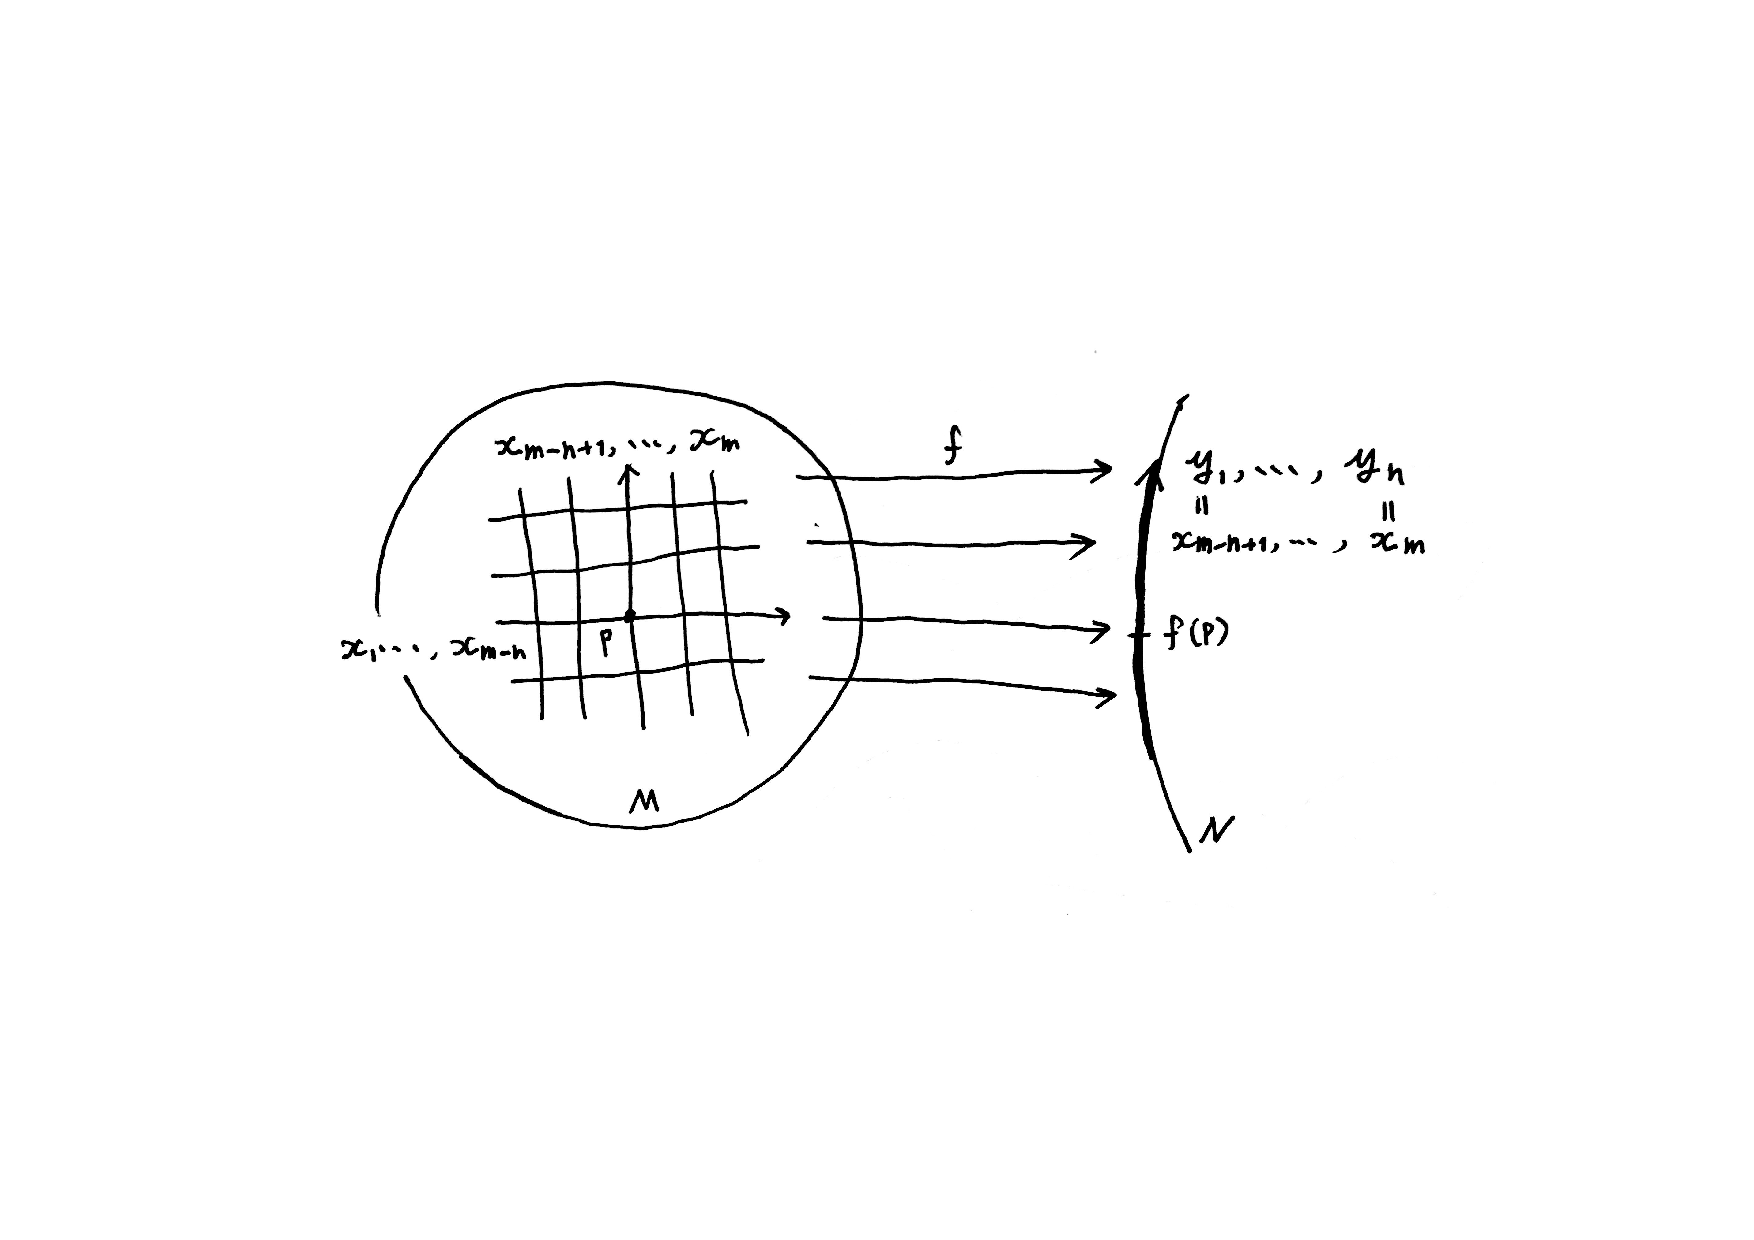
\includegraphics[keepaspectratio, scale=0.5]{projectionTheorem.pdf}
    \caption{射影の様子}
    \label{projectionTheorem}
   \end{figure}
   
\begin{proof}
    $C^r$級写像$f:M\to N$が与えられており, 
    ある点$p\in M$における微分
    $(df)_p:T_p(M)\to T_p(N)$が上への線型写像
    であるとする. このとき, rank$(df)_p=n$
    (ただし, $m=$dim$M\geq n=$dim$N$. )
    点$p$, 点$f(p)$のまわりに, それぞれ座標近傍
    $(U;x_1,\cdots ,x_m)$, $(V;y_1,\cdots ,y_n)$
    をとり, $f$を局所座標表示すると
    $$(y_1, \cdots ,y_n)=(f_1(x_1,\cdots ,x_m), 
    \cdots ,f_n(x_1,\cdots ,x_m))$$
    ヤコビ行列$(Jf)_p$は$(df)_p$を表す行列で, 
    $n$行$m$列である. rank$(df)_p=n$であるから, 
    $(Jf)_p$から$n$本の列ベクトルを選んで, 作った
    正方行列は正則である. 必要なら適当に列を入れ替えて
    $$B=
    \begin{pmatrix}
        \frac{\partial f_1}{\partial x_{m-n+1}}(p) & \cdots & \frac{\partial f_1}{\partial x_m}(p)  \\
        &\cdots& \\
        \frac{\partial f_n}{\partial x_{m-n+1}}(p) & \cdots & \frac{\partial f_n}{\partial x_m}(p)  \\
    \end{pmatrix}
    $$
    とおくと, det$B \neq 0$であって, 
    $$(Jf)_p=
    \left(
        \begin{array}{ccc|c} 
          * & \cdots & *  &  \\
           &  &   & B \\
          * & \cdots & *  & 
        \end{array} 
        \right)
$$
と仮定してよい. $p$のまわりの座標近傍
$(U;x_1,\cdots ,x_m)$から, $\mathbb{R}^m$への
写像$\varphi :U\to \mathbb{R}^m$を
$$\varphi(x_1,\cdots ,x_m)=(x_1, \cdots ,x_{m-n},f_1(x_1,\cdots ,x_m), 
\cdots ,f_n(x_1,\cdots ,x_m))$$
と定義する. やコビ行列$(J\varphi)_p$は
$$(J\varphi)_p=
    \left(
        \begin{array}{ccc|ccc} 
          1 &        &   & & & \\
            & \ddots &   & &O& \\
            &        & 1 & & &  \\ \hline
          * & \cdots & * & & &  \\
            & \cdots &   & &B& \\
          * & \cdots & * & & &
        \end{array} 
        \right)
$$
となり, det$(J\varphi)_p=$det$B\neq 0$である. 
したがって, 逆関数の定理(定理
\ref{theo:f^(-1)theorem})
により, 点$p$を含む$U$を十分小さくとれば, 
$\varphi |U:U\to \varphi(U)$は$C^r$級微分同相写像
である. よって, /ref{prop: cord-nabor condition}
より,$(U, \varphi|U)$は$p$のまわりの新しい$C^r$
級座標近傍と思える. $(U, \varphi|U)$の
局所座標系を$(z_1,\cdots ,z_m)$とすると, 
上の$\varphi$の定義式から, 
$$(z_1,\cdots ,z_m)=\varphi(x_1,\cdots x_m)
=(x_1,\cdots x_{m-n},f_1(x_1,\cdots ,x_m), 
\cdots ,f_n(x_1,\cdots ,x_m))$$
を得る. とくに, $(z_{m-n+1},\cdots ,z_m)
=(f_1(x_1,\cdots ,x_m), 
\cdots ,f_n(x_1,\cdots ,x_m))$
であるから, 
\begin{eqnarray*}
    f\circ \varphi (z_1,\cdots z_m)&=&f(x_1,\cdots x_m)\\
    &=&(f_1(x_1,\cdots ,x_m),\cdots ,f_n(x_1,\cdots ,x_m))\\
    &=&(z_{m-n+1},\cdots ,z_m)
\end{eqnarray*}
となる. よって, $(z_1,\cdots ,z_m)$と$(y_1,\cdots ,y_n)$
に関する$f:M\to N$の点$p$のまわりでの局所座標表示
$$(z_1,\cdots ,z_m)\mapsto (z_{m-n+1},\cdots ,z_m)
=(y_1,\cdots ,y_n)$$
である. $(z_1,\cdots ,z_m)$を改めて$(x_1,\cdots ,x_m)$
と書き直せば, 定理\ref{theo: projection theorem}の
主張が得られる. 
\end{proof}
\begin{theorem}\label{theo:inclusion map theorem}
    $f:M\to N$を$C^r$級写像とする. 
    $(df)_p:T_p(M)\to T_{f(p)}(N)$が
    $1$対$1$の線型写像なら, 点$p$の付近での$f$の
    様子は, 包含写像
    $\mathbb{R}^m\to \mathbb{R}^n,\ 
    (x_1,\cdots ,x_m)\mapsto 
    (x_1,\cdots ,x_m,0,\cdots ,0)$
    と同じである. すなわち, $p$のまわりの局所座標系
    $(x_1,\cdots ,x_m)$と$f(p)$のまわりの局所座標系
    $(y_1,\cdots ,y_n)$をうまく選んで, $f$の
    局所座標表示
    $(y_1,\cdots ,y_n)\mapsto (f_1(x_1,\cdots x_m),
    \cdots ,f_n(x_1,\cdots x_m),)$が, 
    \begin{eqnarray*}
        y_1&=&f_1(x_1,\cdots x_m)=x_1\\
        &\vdots& \\
        y_m&=&f_m(x_1,\cdots x_m)=x_m\\
        y_{m+1}&=&f_{m+1}(x_1,\cdots x_m)=0\\
        &\vdots& \\
        y_n&=&f_n(x_1,\cdots x_m)=0\\
    \end{eqnarray*}
    であるようにできる. 
\end{theorem}
\begin{figure}[H]
    \centering
    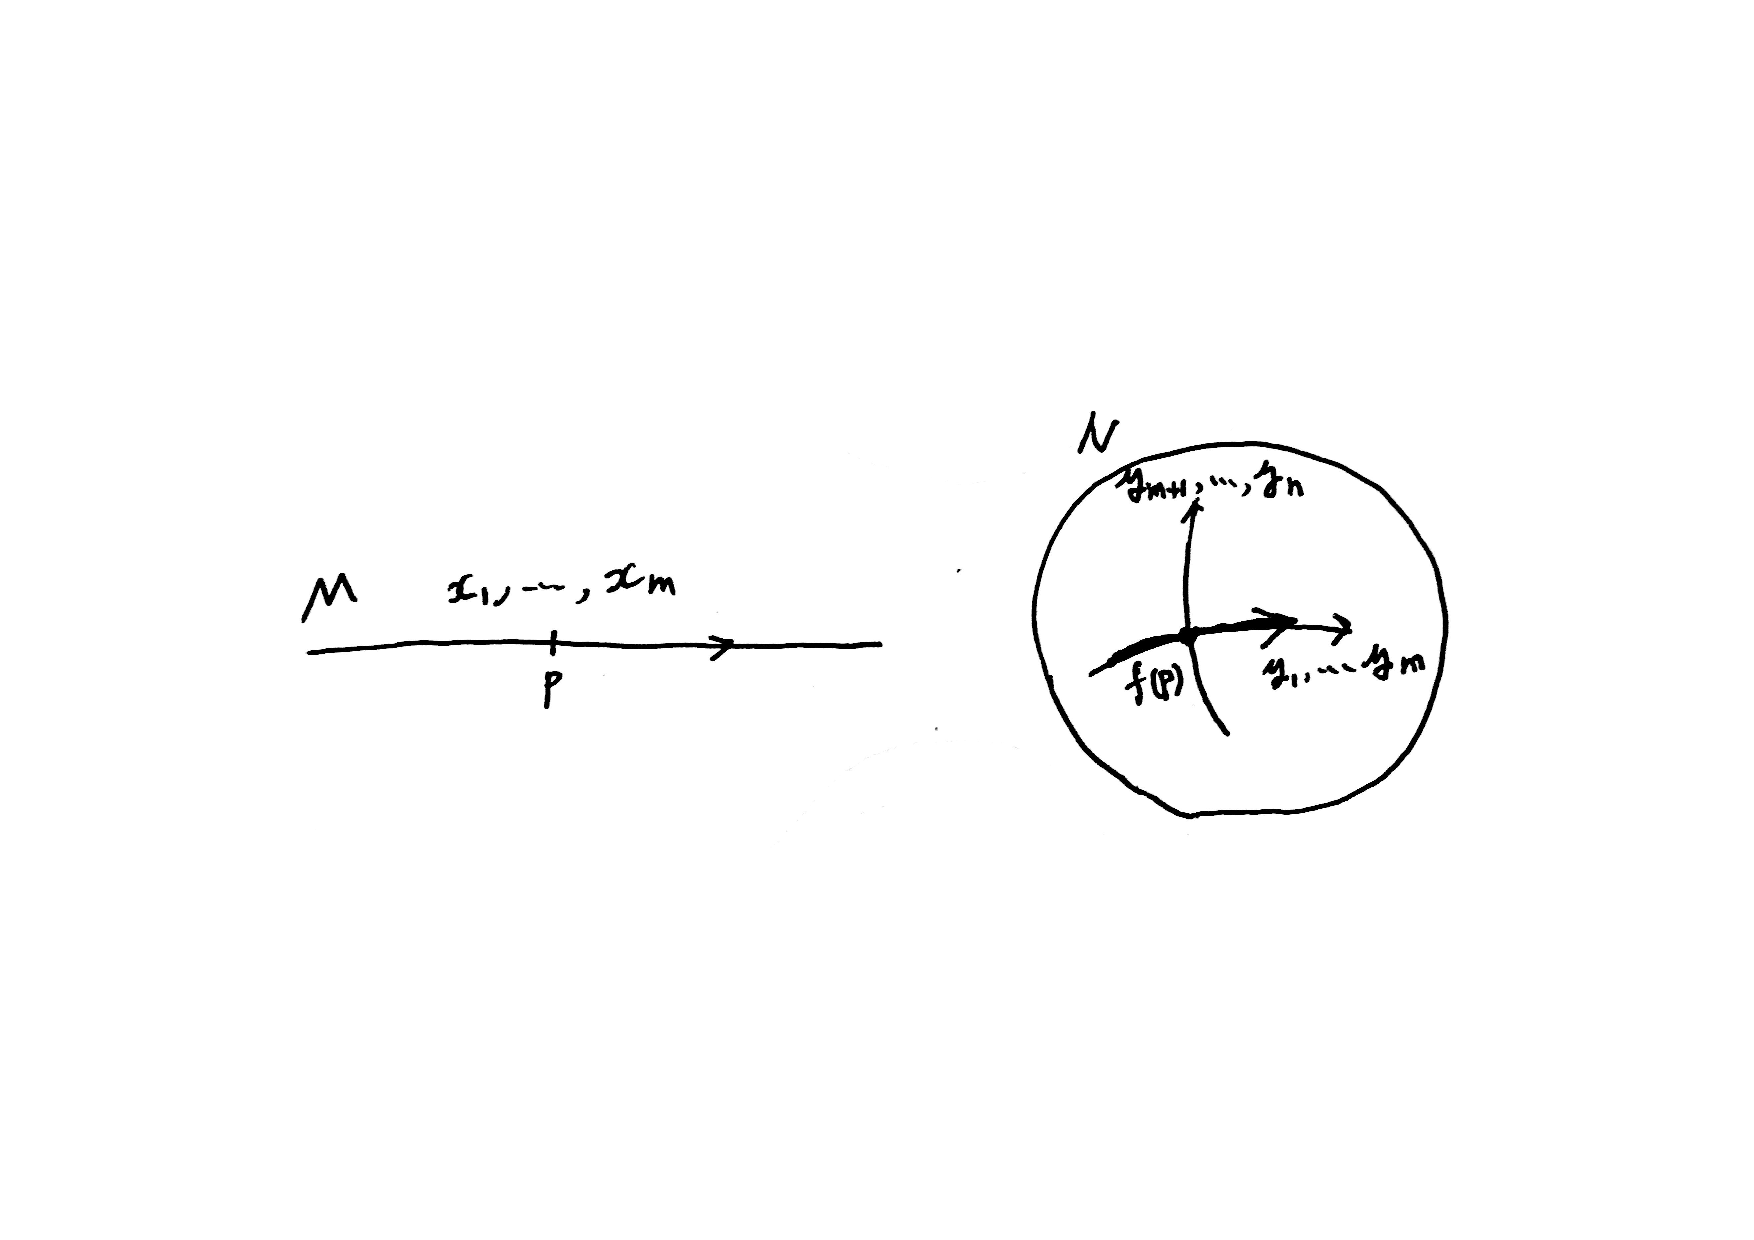
\includegraphics[keepaspectratio, scale=0.5]{subsetmapTheorem.pdf}
    \caption{包含写像の様子}
    \label{subsetmapTheorem}
   \end{figure}
   
\begin{proof}
    問題は局所的であるから$M=\mathbb{R}^m$, 
    $N=\mathbb{R}^n$と仮定してよい. ($m\leq n$)
    また, $p=\boldsymbol{o}$, $f(p)=\boldsymbol{o}$
    としてよい. 
    $\mathbb{R}^m$の自然な座標$(x_1, \cdots ,x_m)$
    と, $\mathbb{R}^n$の自然な座標に関して, 
    与えられた$C^r$級写像$f:\mathbb{R}^m\to \mathbb{R}^n$
    を局所座標表示したものを
    $$u_1=f_1(x_1,\cdots ,x_m),\ \cdots ,
    u_n=f_n(x_1,\cdots ,x_m)$$
    とする. $(df)_{\boldsymbol{o}}:
    T_{\boldsymbol{o}}(\mathbb{R}^m)\to 
    T_{\boldsymbol{o}}(\mathbb{R}^n)$
    は$1$対$1$であるから, ヤコビ行列$(Jf)_{\boldsymbol{o}}$
    から, 適当な$m$行を選び出して作った$m$次正方行列
    は正則である. 必要なら, 
    $(u_1, \cdots ,u_m)$の並び方を変えて, 
    $(Jf)_{\boldsymbol{o}}=
    \begin{pmatrix}
        A \\ \hline
        B
     \end{pmatrix}
     $
     ($A$は$m$行$m$列の正則行列)と仮定してよい. 
     $(x_1, \cdots ,x_m)$に新しく, 
     $(x_{m+1}, \cdots ,x_n)$を付け加えて, 
     $\mathbb{R}^m \times \mathbb{R}^{n-m}$を
     構成し, 新しい写像
     $F:\mathbb{R}^m \times \mathbb{R}^{n-m}
     \to \mathbb{R}^n$
    を, 
    \begin{eqnarray*}
        &&F(x_1,\cdots ,x_m,x_{m+1},\cdots x_n)\\
    &&=(f_1(x_1,\cdots ,x_m),\cdots ,f_m(x_1,\cdots ,x_m), 
    f_{m+1}(x_1,\cdots ,x_m)+x_{m+1}, 
    \cdots ,f_{n}(x_1,\cdots ,x_m)+x_{n})
    \end{eqnarray*}
    と定義する.$F$のヤコビ行列
    $$(Jf)_{\boldsymbol{o}}=
    \left(
\begin{array}{c|ccc} 
  A &  & O  &  \\ \hline
   & 1 &   &  \\
  B &  & \vdots &  \\
   &  &   & 1
\end{array} 
\right)
    $$
    であり, 正則である. 
    逆関数の定理\ref{theo:f^(-1)theorem}により, 
    $\mathbb{R}^m \times \mathbb{R}^{n-m}$
    における, $\boldsymbol{o}$の近傍$U$と, 
    $\mathbb{R}^n$における$\boldsymbol{o}$
    の近傍$V$が存在して, $F|U:U\to V$は$C^r$級
    微分同相写像になる. $\psi =(F|U)^{-1}:V\to U$
    とおく. $(V, \psi)$は$\boldsymbol{o}$の
    まわりの$\mathbb{R}^n$の$C^r$級座標近傍と思える. 
    この座標近傍に関する局所座標系を$(y_1,\cdots y_n)$
    とし, $(x_1, \cdots ,x_m)$と$(y_1,\cdots y_n)$に
    関して, $f:U\cap(\mathbb{R}^m\times 
    \{ \boldsymbol{o} \})\to \mathbb{R}^n$
    を局所座標表示すると, 
    \begin{eqnarray*}
        (y_1,\cdots ,y_n)&=&\psi (f(x_1,\cdots ,x_m))\\
        &=&\psi(F(x_1,\cdots ,x_m,0,\cdots 0))\\
        &=&(F|U)^{-1}(F(x_1,\cdots ,x_m,0,\cdots 0))\\
        &=&(x_1,\cdots ,x_m,0,\cdots ,0)
    \end{eqnarray*}
    となる. したがって, 定理\ref{theo:inclusion map theorem}
    の主張する通りの局所座標表示が得られた. 
\end{proof}
\subsection{$C^r$級部分多様体}
\begin{definition}\label{def:C^r-submanifold}
    $n$次元$C^r$級多様体$N$の部分集合$L$が
    $N$の$l$次元$C^r$級部分多様体であるとは, 
    \begin{itemize}
        \item[(1)]$l=n$のとき:$L$が$N$の開集合
        であることである. 
        \item[(2)] $0\leq l<n$のとき:$L$の任意の点$p$
        に対し, $p$を含む$N$の座標近傍$(U;x_1,\cdots ,x_n)$
        が存在して, 
        $$L\cap N=\{(x_1,\cdots ,x_n)\in U|
        x_{l+1}=\cdots =x_n=0\}$$
        が成り立つことである. 
    \end{itemize}
\end{definition}
\begin{figure}[H]
    \centering
    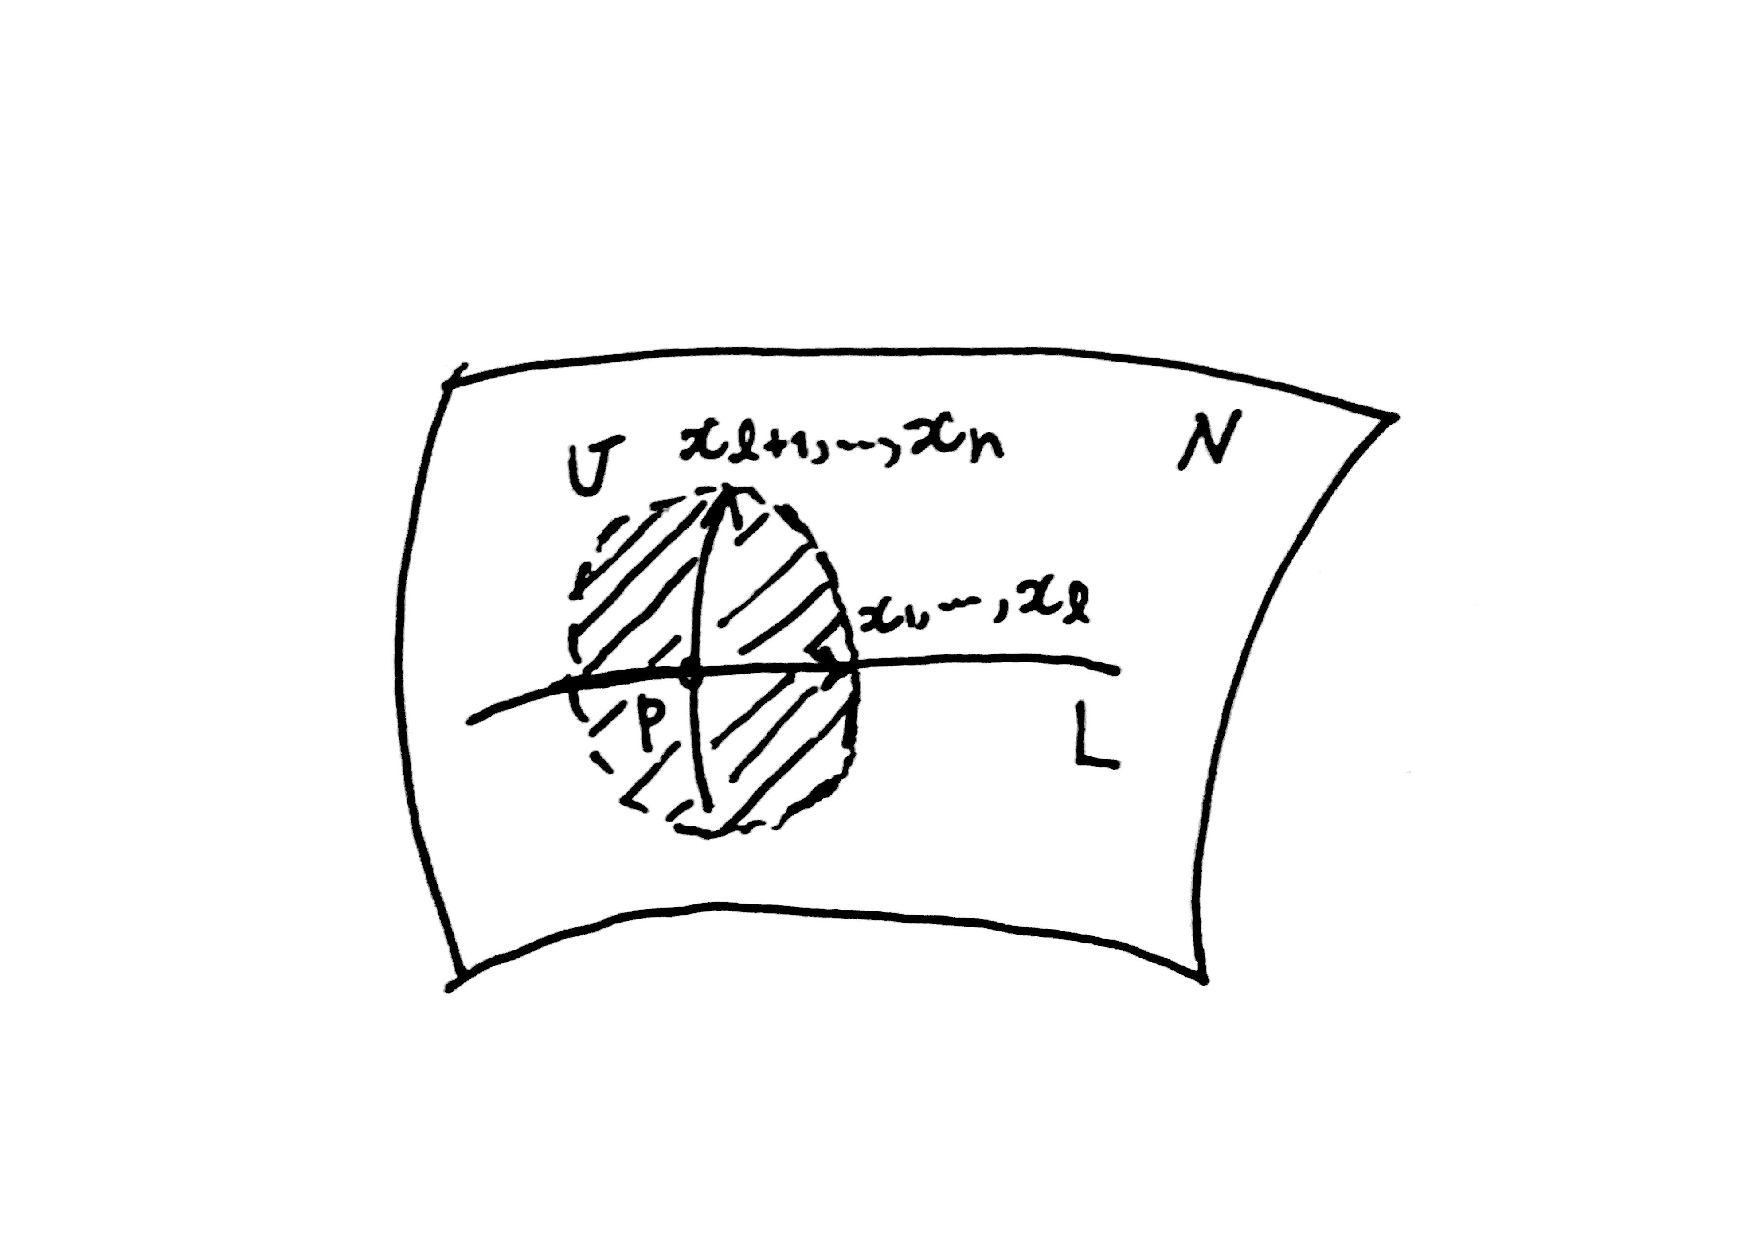
\includegraphics[keepaspectratio, scale=0.4]{CrSubmanifold.pdf}
    \caption{$N$の部分多様体$L$}
    \label{CrSubmanifold}
   \end{figure}
   
\begin{proposition}\label{prop:dim of C^r-submanifold}
    $n$次元$C^r$級多様体$N$の$l$次元$C^r$級
    部分多様体$L$は, それ自身$l$次元$C^r$級
    多様体である. 
\end{proposition}
\begin{proof}
    \begin{itemize}
        \item[(1)]
        $l=n$のとき, $N$からの相対位相によって, 
        $L$は位相空間となり, 
        $N$の$C^r$級座標近傍を
        $\mathcal{S}=
        \{U_\alpha,\varphi _\alpha\}_{\alpha\in A}$
        とすると, $\mathcal{S}$を$L$に制限した
        $\{U_\alpha \cap L,
        \varphi _\alpha |U_\alpha \cap L\}_{\alpha\in A}$
        は$L$の$C^r$局所座標系になる. 
        よって, $L$はそれ自身, $l$($=n$)次元
        $C^r$級多様体である. 
        \item[(2)] 
        $0\leq l<n$のとき, $L$には$N$からの相対位相
        を入れる. $N$がハウスドルフ空間であるから$L$
        もそうである. \\
        $L$の任意の点$p$に対し, $p$を含む$N$の
        局所座標系$(U;x_1,\cdots ,x_n)$で定義
        \ref{def:C^r-submanifold}の条件を満たすもの
        を選び, $(U_p;x^p_1,\cdots ,x^p_n)$とする. 
        $V_p=L\cap U_p$とおくと, $V_p$は$L$の開集合
        である. $V_p$上の$U_p$の局所座標系
        $(x^p_1, \cdots ,x^p_n)$の$x^p_1$から
        $x^p_l$までを制限したもの$(V_p;x^p_1,\cdots ,x^p_l)$
        を考える. \\
        $\{(V_p;x^p_1,\cdots ,x^p_l)\}_{p\in L}$が
        $L$を被覆することは明らかである.\\
        $V_p$と$V_q$が交わるとする. 対応する
        $(U_p;x^p_1,\cdots ,x^p_n)$ と
        $(U_q;x^q_1,\cdots ,x^q_n)$は, 
        $N$の適当な座標近傍
        $(U_\alpha ;x^\alpha_1, \cdots ,x^\alpha_n)$,
        $(U_\beta ;x^\beta_1, \cdots ,x^\beta_n)$
        である. この間の座標変換はある$C^r$級関数$f$を
        用いて, 
        $$(x^\beta_1, \cdots ,x^\beta_n)
        =(f_1(x^\alpha_1, \cdots ,x^\alpha_n), \cdots 
        , f_n(x^\alpha_1, \cdots ,x^\alpha_n))$$
        と書ける. $V_p\cap V_q$上では, 
        $x^\alpha_{l+1}=\cdots =x^\alpha_n=0$, $x^\beta_{l+1}=\cdots =x^\beta_n=0$
        が成り立つので, $V_p\cap V_q$上では
        \begin{eqnarray*}
            x^\beta_1&=&f_1(x^\alpha_1, \cdots ,x^\alpha_l,0,\cdots ,0)\\
            &\vdots& \\
            x^\beta_l&=&f_l(x^\alpha_1, \cdots ,x^\alpha_l,0,\cdots ,0)\\
            0&=&f_{l+1}(x^\alpha_1, \cdots ,x^\alpha_l,0,\cdots ,0)\\
            &\vdots& \\
            0&=&f_n(x^\alpha_1, \cdots ,x^\alpha_l,0,\cdots ,0)\\
        \end{eqnarray*}
        となっている. 改めて関数$g$を
        \begin{eqnarray*}
            g(x^\alpha_1, \cdots ,x^\alpha_l)&=&
            (g_1(x^\alpha_1, \cdots ,x^\alpha_l), \cdots 
            , g_l(x^\alpha_1, \cdots ,x^\alpha_l))\\
            &=&(f_1(x^\alpha_1, \cdots ,x^\alpha_l,0,\cdots ,0), \cdots 
            , f_l(x^\alpha_1, \cdots ,x^\alpha_l,0,\cdots ,0))
        \end{eqnarray*}
        と定義すると, この関数は$C^r$級である. 
        そして, 
        $$(x^\beta_1, \cdots ,x^\beta_l)
        =g(x^\alpha_1, \cdots ,x^\alpha_l)$$
        が$(V_p;x^p_1,\cdots x^p_l)$から
        $(V_q;x^q_1,\cdots x^q_l)$の座標変換を与えている. \\
        ゆえに, $\{(V_p;x^p_1,\cdots ,x^p_l)\}_{p\in L}$
        は$L$の$C^r$級座標近傍になっている. \\
        以上より, $L$は$l$次元$C^r$級多様体である. 
    \end{itemize}
\end{proof}
\begin{theorem}\label{theo:f^{-1}(q) C^r manifold}
    $M$, $N$を$m$次元, $n$次元の$C^r$級多様体, 
    $f:M\to N$を$C^r$級写像とする. $N$のある点
    $q$について, $f(p)=q$となる$M$の各点$p$
    が常にrank$(Jf)_p=n$を満たすとき, 逆像
    $f^{-1}(q)$は$(m-n)$次元$C^r$級多様体
    である. 
\end{theorem}
\begin{proof}
    定義\ref{def:C^r-submanifold}, 命題
    \ref{prop:dim of C^r-submanifold}より, 
    次のことを証明すればよい.\\ 

    $q\in N$の逆像$f^{-1}(q)$に属する任意の点
    $p$に対し, $p$のまわりの座標近傍
    $(U;x_1,\cdots .x_m)$が存在して, 
    $$f^{-1}(q)\cap U
    =\{(x_1,\cdots x_m)\in U|
    x_{m-n+1}=\cdots =x_m=0\}$$
    が成り立つ. \\

    今, $f(p)=q$を満たす$p\in M$について, 常に
    rank$(Jf)_p=n$であるから, $(df)_p$は上への
    写像である. よって, 定理\ref{theo: projection theorem}
    より, $p$のまわりの座標近傍$(U;x_1,\cdots ,x_m)$
    と$q$($=f(p)$)のまわりの座標近傍
    $(V;y_1,\cdots ,y_n)$が存在して, $f|U:U\to V$
    は
    $$(y_1,\cdots ,y_n)=f(x_1,\cdots x_m)
    =(x_{m-n+1},\cdots ,x_m)$$
    と座標表示される. \\
    $(U;x_1,\cdots x_m)$は任意にとってきた
    $(V;y_1,\cdots ,y_n)$
    に応じて選べるから, $(V;y_1,\cdots ,y_n)$は
    点$q$で$y_1=\cdots =y_n=0$となるように
    とっておくと, 
    \begin{eqnarray*}
        f^{-1}(q)\cap U&=& \{p\in U|f(p)=q\}\\
        &=&\{(x_1,\cdots ,x_m)\in U|f(x_1,\cdots x_m)=(0,\cdots ,0)\}\\
        &=&\{(x_1,\cdots ,x_m)\in U|(x_{m-n+1},\cdots x_m)=(0,\cdots ,0)\}\\
        &=&\{(x_1,\cdots x_m)\in U|x_{m-n+1}=\cdots =x_m=0\}
    \end{eqnarray*}
    となり, 条件を満たす$U$が存在することがわかる. 
    これで定理\ref{theo:f^{-1}(q) C^r manifold}
    が証明できた. 
\end{proof}
\subsection{多様体の次元の具体的な計算}
最後に定理\ref{theo:f^{-1}(q) C^r manifold}を
用いて多様体の次元を具体的に計算していく. 
\begin{example}
    $n$次元球面
    $$S^n=\{(x_1,\cdots ,x_{n+1}\in 
    \mathbb{R}^{n+1})|x_1^2+\cdots +x_{n+1}^2=1\}$$
    は$n$次元$C^\infty$級多様体である. 

    $C^\infty$級写像($C^\infty$級関数)
    $f:\mathbb{R}^{n+1}\to \mathbb{R}$を
    $$f(x_1,\cdots ,x_{n+1})=
    x_1^2+\cdots +x_{n+1}^2-1$$
    で定義すると, 
    $$S^n=\{(x_1,\cdots ,x_{n+1}\in 
    \mathbb{R}^{n+1})|f(x_1,\cdots ,x_{n+1})=0\}
    =f^{-1}(0)$$
    より, $S^n$は逆像$f^{-1}(0)$となっている. 
    ヤコビ行列$(Jf)_{\boldsymbol{x}}$を調べると, 
    \begin{eqnarray*}
        (Jf)_{\boldsymbol{x}}&=&
    \left(\frac{\partial f}{\partial x_1}
    (\boldsymbol{x}), 
    \cdots ,\frac{\partial f}{\partial x_{n+1}}
    (\boldsymbol{x})\right)\\
    &=&(2x_1,\cdots ,2x_{n+1})
    \end{eqnarray*}
    $\boldsymbol{x}=(x_1,\cdots x_{n+1})\in S^n$
    のとき, $\boldsymbol{x}\neq \boldsymbol{o}
    \ (:=(0, \cdots ,0))$であるから, 
    $$(Jf)_{\boldsymbol{x}}=(2x_1,\cdots ,2x_{n+1})
    \neq \boldsymbol{o}$$
    となり, $(Jf)_{\boldsymbol{x}}$の階数は$1$となる. 
    よって, $S^n$は$(n+1)-1=n$次元$C^\infty$級
    多様体である. 
\end{example}
\begin{example}
    $2$次元トーラス
    $$T^2:=S^1\times S^1=
    \{(\boldsymbol{x},\boldsymbol{y})|
    \boldsymbol{x},\boldsymbol{y}\in S^1\}$$
    は$2$次元$C^\infty$級多様体である. 
    \begin{figure}[H]
        \centering
        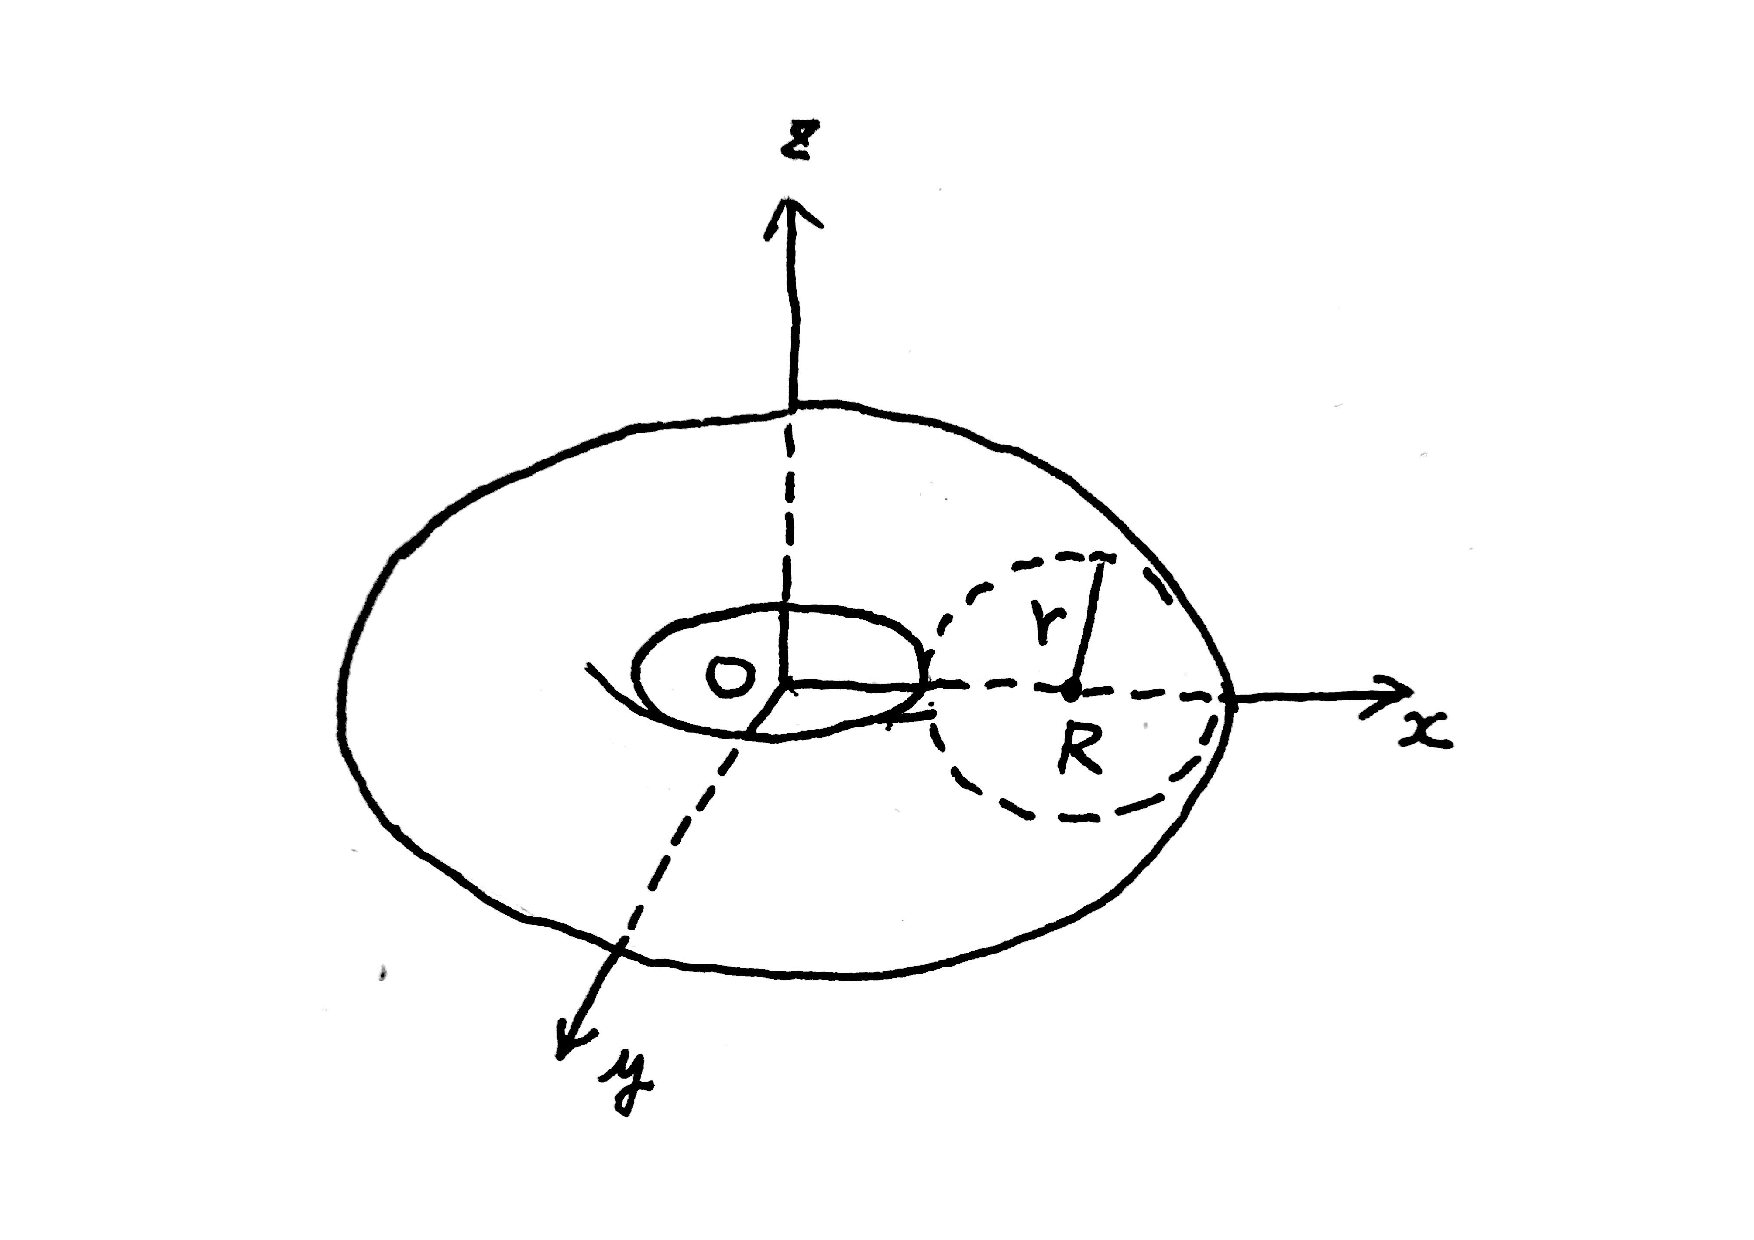
\includegraphics[keepaspectratio, scale=0.4]{T2Noshadow.pdf}
        \caption{$\mathbb{R}^3$の
        中の$2$次元トーラス$T^2$}
        \label{T2Noshadow}
       \end{figure}
    $2$次元トーラス$T^2$は$\mathbb{R}^3$の
    中で$xz$平面上の中心が$(R,0)$, 半径が$r$
    の円を$z$軸のまわりに$1$回転させた図形
    (ただし, $(0<r<R)$)と考えられる
    (図\ref{T2Noshadow})ので, 
    $$T^2=\{(x,y,z)\in \mathbb{R}^3|
    (\sqrt{x^2+y^2}-R)^2+z^2=r^2\}\ (0<r<R)$$
    と表すことができる. 
    $C^\infty$級写像($C^\infty$級関数)
    $f:\mathbb{R}^3\to \mathbb{R}$
    を
    $$f(x,y,z)=(\sqrt{x^2+y^2}-R)^2+z^2-r^2$$
    と定義すると, 
    $$T^2=f^{-1}(0)$$
    となる. $\boldsymbol{p}=(x,y,z)$における
    ヤコビ行列
    $(Jf)_{\boldsymbol{p}}$を調べると, 
    \begin{eqnarray*}
        (Jf)_{\boldsymbol{p}}&=&
        \left(\frac{\partial f}{\partial x}
        (\boldsymbol{p}), \frac{\partial f}{\partial y}
        (\boldsymbol{p}), \frac{\partial f}{\partial z}
        (\boldsymbol{p})\right)\\
        &=&
        \left(\frac{2(\sqrt{x^2+y^2}-R)x}
        {sqrt{x^2+y^2}},\frac{2(\sqrt{x^2+y^2}-R)y}
        {sqrt{x^2+y^2}},2z\right)
    \end{eqnarray*}
    であり, $\boldsymbol{p}\in T^2$のとき, 
    $\boldsymbol{p}\neq \boldsymbol{o}$
    つまり, 常に$x\neq 0$または$y\neq 0$または
    $z\neq 0$が成り立ち, 
    $\sqrt{x^2+y^2}-R=0$のときは$z=\pm r\neq 0$
    となる. よって, 
    $$(Jf)_{\boldsymbol{p}}=
    \left(\frac{2(\sqrt{x^2+y^2}-R)x}
        {\sqrt{x^2+y^2}},\frac{2(\sqrt{x^2+y^2}-R)y}
        {\sqrt{x^2+y^2}},2z\right)\neq 
        \boldsymbol{o}$$
    となり, rank$(Jf)_{\boldsymbol{p}}=1$
    を得る. 
    したがって, $T^2$は$3-1=2$次元$C^\infty$
    級多様体である. 
\end{example}
\begin{example}
    $S^1 \subset \mathbb{R}^2$であることに注意する
    と$2$次元トーラス$T^2$は
    $\mathbb{R}^4$の部分集合として, 
    $$T^2=\{(x_1,x_2,x_3,x_4)\in \mathbb{R}^4|
    x_1^2+x_2^2=1, x_3^2+x_4^2=1\}$$
    と表せる. この表し方においても$T^2$は
    $2$次元$C^\infty$級多様体になる. 

    $C^\infty$級写像$f:\mathbb{R}^4\to \mathbb{R}^2$
    を
    $$f(x_1,x_2,x_3,x_4)=(x_1^2+x_2^2-1,
    x_3^2+x_4^2-1)$$と定義すると, 
    $$T^2=f^{-1}(0,0)$$
    と表せる. 点$\boldsymbol{p}=(x_1,x_2,x_3,x_4)$
    におけるヤコビ行列$(Jf)_{\boldsymbol{p}}$
    を調べると, 
    \begin{eqnarray*}
        (Jf)_{\boldsymbol{p}}&=&
        \left(\begin{array}{cccc}
            \frac{\partial f_1}{\partial x_1}&
            \frac{\partial f_1}{\partial x_2}&
            \frac{\partial f_1}{\partial x_3}&
            \frac{\partial f_1}{\partial x_4}\\
            \frac{\partial f_2}{\partial x_1}&
            \frac{\partial f_2}{\partial x_2}&
            \frac{\partial f_2}{\partial x_3}&
            \frac{\partial f_2}{\partial x_4}
        \end{array}\right)\\
        &=&
        \left(\begin{array}{cccc}
            2x_1&2x_2&0&0\\
            0&0&2x_3&2x_4
        \end{array}\right)
    \end{eqnarray*}
    $\boldsymbol{p}\in T^2$のとき, $x_1\neq 0$
    または$x_2\neq 0$で, さらに$x_3\neq 0$または
    $x_4\neq 0$でもあるので, $(Jf)_{\boldsymbol{p}}$
    の$2$つの行ベクトル$(2x_1,2x_2,0,0)$, 
    $(0,0,2x_3,2x_4)$は$1$次独立である. 行列の
    階数はその行列の$1$次独立な行ベクトルの個数
    に一致するから, rank$(Jf)_{\boldsymbol{p}}=2$
    である. 
    よって, $T^2$は$4-2=2$次元$C^\infty$級
    多様体である. 
\end{example}
\begin{example}
    らせん$H=\{(x,y,z)\in \mathbb{R}^3|
    x=\cos z, y=\sin z\}$は
    $1$次元$C^\infty$級多様体である. 

    $C^\infty$級写像$\mathbb{R}^3\to \mathbb{R}^2$
    を
    $$f(x,y,z)=(x-\cos z,y-\sin z)$$
    と定義すると, 
    $$H=f^{-1}(0,0)$$
    となる. 点$\boldsymbol{p}=(x,y,z)$
    におけるヤコビ行列$(Jf)_{\boldsymbol{p}}$
    を調べると, 
    \begin{eqnarray*}
        (Jf)_{\boldsymbol{p}}&=&
        \left(\begin{array}{ccc}
            \frac{\partial f_1}{\partial x}&
            \frac{\partial f_1}{\partial y}&
            \frac{\partial f_1}{\partial z}\\
            \frac{\partial f_2}{\partial x}&
            \frac{\partial f_2}{\partial y}&
            \frac{\partial f_2}{\partial z}
        \end{array}\right)\\
        &=&
        \left(\begin{array}{ccc}
            1&0&\sin z\\
            0&1&-\cos z
        \end{array}\right)
    \end{eqnarray*}
    となる. $(Jf)_{\boldsymbol{p}}$
    の$2$つの行ベクトル$(1,0,\sin z)$, 
    $(0,1,-\cos z)$は$1$次独立であるから, 
    rank$(Jf)_{\boldsymbol{p}}=2$
    よって, $H$は$3-2=1$次元$C^\infty$級
    多様体である. 
\end{example}
\begin{definition}\label{def:Stiefel manifold}
    $\mathbb{R}^m$の直交$k$枠とは, $\mathbb{R}^m$
    の中の$k$個のベクトルの組$(\boldsymbol{v}_1,
    \cdots ,\boldsymbol{v}_k)$であって, 
    次の条件(1), (2)を満たすものをいう. 
    (ただし, $1\leq k\leq m$とする. )
    \begin{itemize}
        \item[(1)]
        $\|\boldsymbol{v}_i\|=1\ (i=1,\cdots ,k)$
        \item[(2)] 
        $\boldsymbol{v}_i$と$\boldsymbol{v}_j$は
        直交する. ($i\neq j,\ i,j=1,\cdots k$)
    \end{itemize}
    \begin{figure}[H]
        \centering
        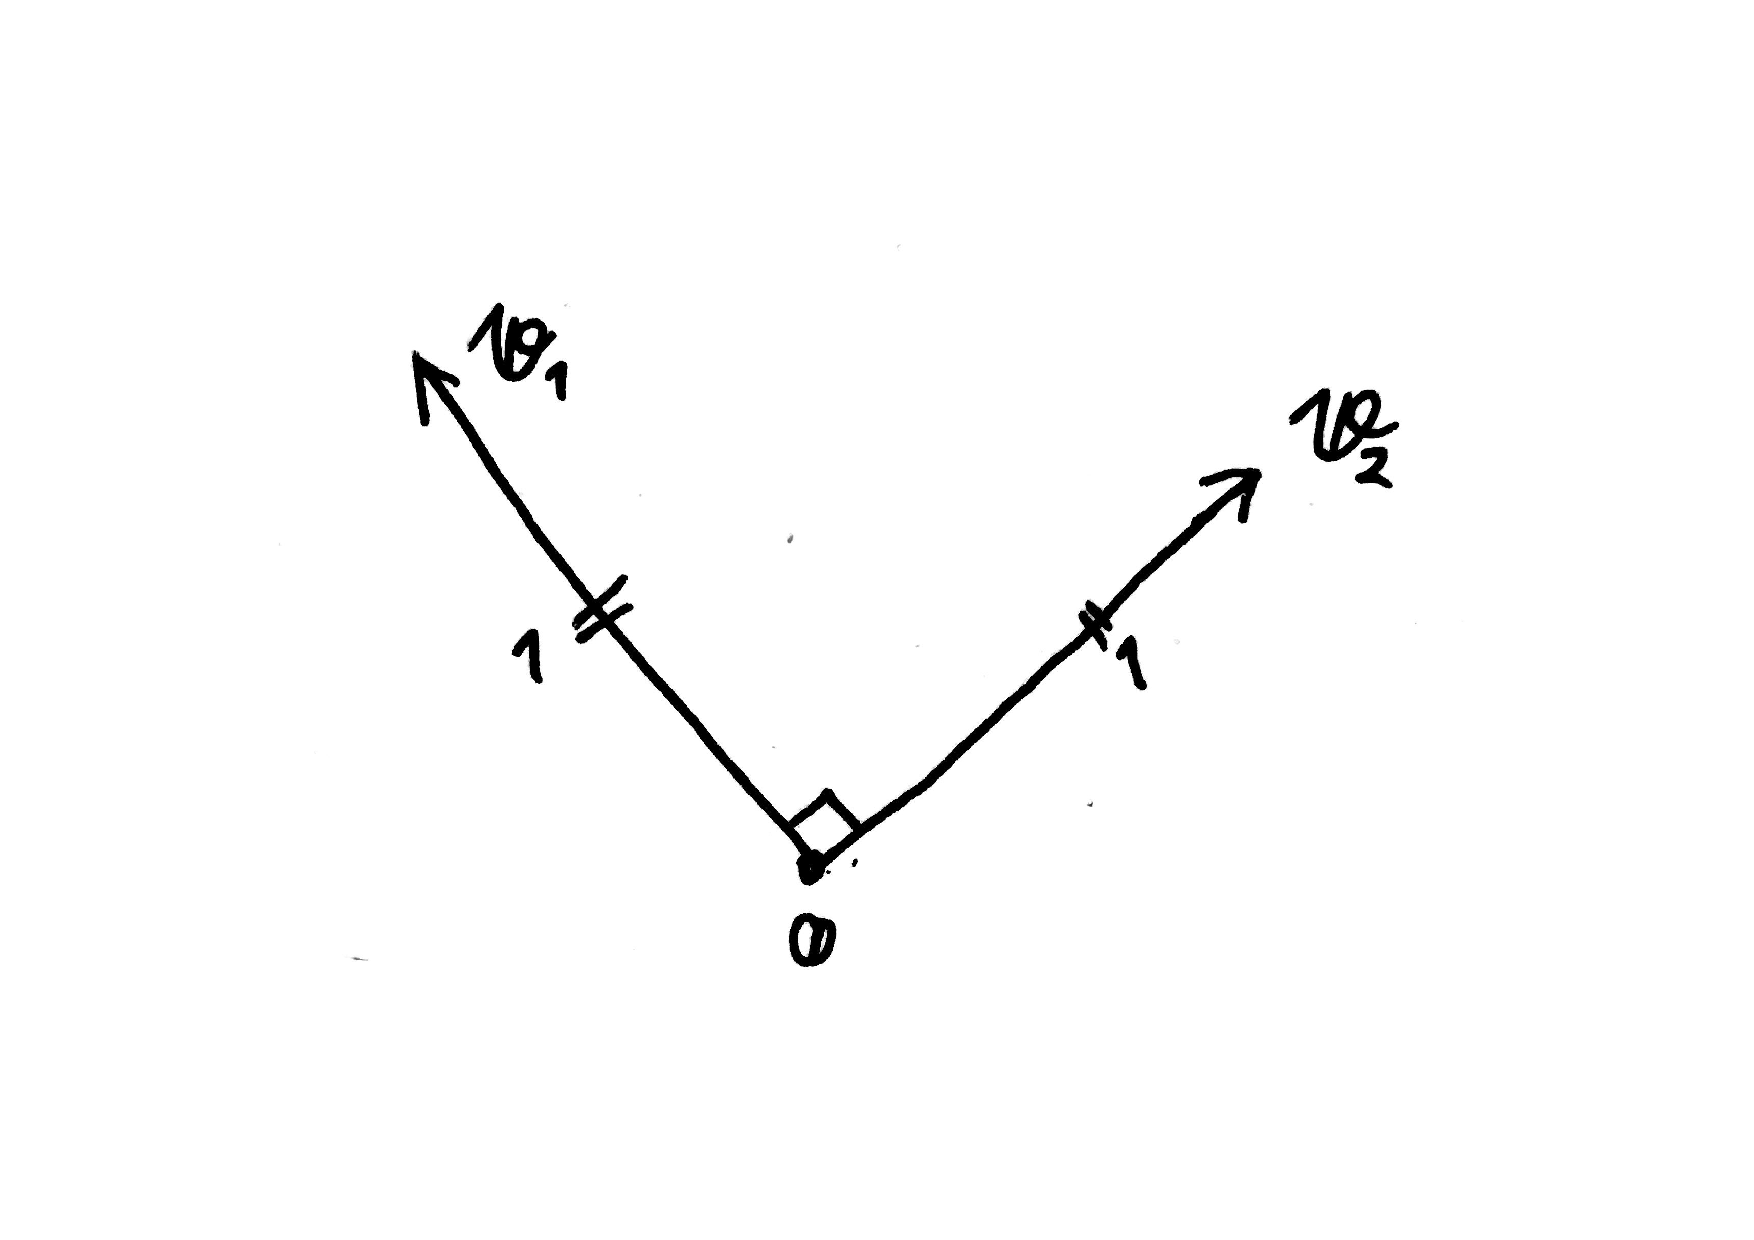
\includegraphics[keepaspectratio, scale=0.3]{orthogonalKframe.pdf}
        \caption{直交$2$枠$(\boldsymbol{v}_1,
        \boldsymbol{v}_2)$}
        \label{orthogonalKframe}
       \end{figure}
    $\mathbb{R}^m$の中の直交$k$枠の全体のなす
    集合を
    $$V_{m,k}$$
    と表し, ($m,k$)型のシュティーフェル多様体とよぶ. 
\end{definition}
以下, $m=2$のときのシュティーフェル多様体$V_{2,k}$
を調べる. 
\begin{example}
    $k=1$のとき, 
    シュティーフェル多様体$V_{2,1}$は
    $1$次元$C^\infty$級多様体になる. 

    定義より, 
    \begin{eqnarray*}
        V_{2,1}&=&\{\boldsymbol{v}\in
    \mathbb{R}^2|\|\boldsymbol{v}\|=1\}\\
    &=&\{(v_1,v_2)\in
    \mathbb{R}^2|v_1^2+v_2^2=1\}=S^1
    \end{eqnarray*}
    となり, $V_{2,1}$は$1$次元球面$S^1$と等しい
    ことがわかる. よって$V_{2,1}$は
    $1$次元$C^\infty$級多様体になる.
\end{example}
\begin{example}\label{ex:(2,2)Stiefel manifold}
    $k=2$のとき, 
    シュティーフェル多様体$V_{2,2}$は
    $1$次元$C^\infty$級多様体になる. 

    $\boldsymbol{v}_1=(x_1,x_2)$, 
    $\boldsymbol{v}_2=(y_1,y_2)$を
    $\mathbb{R}^2$の直交$2$枠の
    $2$つのベクトルとすると, 定義\ref{def:Stiefel manifold}
    の条件(1), (2)はそれぞれ次のように表せる. 
    \begin{itemize}
        \item[(1)]
        $x_1^2+x_2^2=1, y_1^2+y_2^2=1$
        \item[(2)]
        $x_1y_1+x_2y_2=0$
    \end{itemize}
    よって$V_{2,2}$は
    $$V_{2,2}=\{(x_1,x_2,y_1,y_2)\in \mathbb{R}^4|
    x_1^2+x_2^2=1, y_1^2+y_2^2=1, x_1y_1+x_2y_2=0\}$$
    と書き表せる. 
    $C^\infty$写像$f:\mathbb{R}^4\to \mathbb{R}^3$
    を
    $$f(x_1,x_2,y_1,y_2)=
    (x_1^2+x_2^2-1, y_1^2+y_2^2-1, x_1y_1+x_2y_2)$$
    と定義すると, 
    $$V_{2,2}=f^{-1}(0,0,0)$$
    となる. 点$(\boldsymbol{v}_1,
    \boldsymbol{v}_2)$におけるヤコビ行列
    $(Jf)_{(\boldsymbol{v}_1,
    \boldsymbol{v}_2)}$を計算すると, 
    $$(Jf)_{(\boldsymbol{v}_1,
    \boldsymbol{v}_2)}=
    \left(\begin{array}{cccc}
        2x_1&2x_2&0&0\\
        0&0&2y_1&2y_2\\
        y_1&y_2&x_1&x_2\\
    \end{array}\right)$$
    $(Jf)_{(\boldsymbol{v}_1,
    \boldsymbol{v}_2)}$の$3$つの
    行ベクトル$(2x_1,2x_2,0,0)$, 
    $(0,0,2y_1,2y_2)$, 
    $(y_1,y_2,x_1,x_2)$が$1$次独立である
    ことを示す. $a$, $b$, $c$を実数として, 
    $$a(2x_1,2x_2,0,0)+b(0,0,2y_1,2y_2)+
    c(y_1,y_2,x_1,x_2)=(0,0,0,0)$$
    と仮定すると, 
    $$2a(\boldsymbol{v}_1,0,0)+
    2b(0,0,\boldsymbol{v}_2)+
    c(\boldsymbol{v}_2,\boldsymbol{v}_1)=
    (0,0,0,0)$$
    であるから, これを整理して, 
    $$(2a\boldsymbol{v}_1+c\boldsymbol{v}_2,
    2b\boldsymbol{v}_2+c\boldsymbol{v}_1)=
    (0,0,0,0)$$
    を得る. よって, 
    $$2a\boldsymbol{v}_1+c\boldsymbol{v}_2=
    (0,0),\ 
    2b\boldsymbol{v}_2+c\boldsymbol{v}_1=
    (0,0)$$
    となるが, いま, $\boldsymbol{v}_1$と
    $\boldsymbol{v}_2$は$1$次独立であるから, 
    $a=c=0$, $b=c=0$が導かれ, $a=b=c=0$である
    ことがわかる. したがって, $(2x_1,2x_2,0,0)$, 
    $(0,0,2y_1,2y_2)$, 
    $(y_1,y_2,x_1,x_2)$は$1$次独立である. 
    ゆえに, rank$(Jf)_{(\boldsymbol{v}_1,
    \boldsymbol{v}_2)}=3$であるから, 
    $V_{2,2}$は$4-3=1$次元$C^\infty$級多様体
    となる. 
\end{example}
\newpage
%
\section{おわりに}
本研究の目的は, 直観的に理解し難い
高次元の空間などの
形を理解するために, 
その空間の多様体としての次元を
調べる方法を示すことであった. 

研究の方法としては, 主に$3$つの文献
松本\cite{Matsumoto18}, 藤岡
\cite{Hujioka17}, 服部
\cite{Hattori76}を参考にして, 
必要な定義や定理などの概念を選び, 
論理を構成した. 

その結果, 
空間を多様体$M$, $N$の間の$C^r$級写像$f:M\to N$の逆像$f^{-1}(q)$
(ただし$q$は$N$のある$1$点)
とみなせれば, $f$のヤコビ行列の階数を計算することで
多様体としての次元を調べることができるという
ことが分かり(定理\ref{theo:f^{-1}(q) C^r manifold}), 
その定理を用いて実際に多様体の
次元の具体的な計算を示すことができた. 

今後の課題としては, 多様体が
部分多様体として実現できる空間の
条件(埋め込み可能性)について調べたい. 例えば例
\ref{ex:(2,2)Stiefel manifold}の$V_{2,2}$
は$\mathbb{R}^4$の中の$1$次元部分多様体であると
みなせるが, $V_{2,2}$がより低い次元の
$\mathbb{R}^3$や$\mathbb{R}^2$に埋め込める
かどうかを判定する方法などを調べていきたい. 

\section{謝辞}
最後に, 本論文の作成にあたり, 
指導教員の亀子正喜教授には終始適切な助言をいただきながら
研究を進め, 本論文を書き上げることができました. 
ここに感謝いたします. 
% \begin{figure}[H]
% \end{figure}
\newpage
%参考文献
\begin{thebibliography}{99}
\bibitem{Matsumoto18} 松本幸夫, [第30版]多様体の基礎, 東京大学出版会, 2018.
\bibitem{Hujioka17} 藤岡敦, [第2版]具体例から学ぶ 多様体, 裳華房, 2017.
\bibitem{Hattori76} 服部晶夫, [第1版]多様体, 岩波書店, 1976.
%\bibitem{b}【論文の場合】著者名,タイトル,雑誌名,巻・号,出版年度,頁.
%\bibitem{c}【Webページの場合】 タイトル,ページ制作者(機関)等,URL: \url{http://www.shibaura-it.ac.jp/},最終アクセス日時: 2021/12/28 16:33.
\end{thebibliography}

\end{document}